\documentclass[a4paper,12pt,twoside]{book}
\usepackage[utf8]{inputenc}
\usepackage[english]{babel}
%\usepackage{fontspec}
%\setmainfont[
%  Ligatures=TeX,
%  Extension=.otf,
%  BoldFont=cmunbx,
%  ItalicFont=cmunti,
%  BoldItalicFont=cmunbi,
%  SlantedFont=cmunsl
%]{cmunrm}

%\usepackage{polyglossia}
%\setmainlanguage{spanish}

\usepackage[c5paper]{geometry}
%\geometry{inner=2.5cm,outer=2.5cm,bmargin=3.2cm}
%\usepackage[DIV=14,BCOR=2mm,headinclude=true,footinclude=false]{typearea}

%\usepackage{ulem} %Hace que \emph sea subrayar

%\usepackage[p,osf]{scholax}
%% T1 and textcomp are loaded by package. Change that here, if you want
%% load sans and typewriter packages here, if needed

\usepackage{ebgaramond}
%\usepackage[type1]{libertine} % Linux Libertine for zweispaltige Texte
%\usepackage{textcomp}% Required to get special symbols
\usepackage[scaled=.8]{DejaVuSansMono}% FiraMono Typewriter font
\usepackage{PTSansNarrow} 
%\gilliuscondensed
%\usepackage[sfdefault]{FiraSans}
%\usepackage{bm}% Extra bold faces
%\usepackage[lf]{carlito}

\usepackage{lettrine} %Capital letters at the beginning of a chapter
\usepackage[activate={true,nocompatibility},final,tracking=true,kerning=true,spacing=true,factor=1100,stretch=10,shrink=10]{microtype}
\SetTracking{encoding={*}, shape=sc}{-20} % versalitas menos separadas
% activate={true,nocompatibility} - activate protrusion and expansion
% final - enable microtype; use "draft" to disable
% tracking=true, kerning=true, spacing=true - activate these techniques
% factor=1100 - add 10% to the protrusion amount (default is 1000)
% stretch=10, shrink=10 - reduce stretchability/shrinkability (default is 20/20)

%\usepackage{array,multirow,booktabs,colortbl,chngcntr} % El último es para counterwithout;
\usepackage[strict]{changepage}
%\usepackage{caption}
%\captionsetup{format=plain,labelsep=newline,labelfont={small,sc},
%textfont={small,it},singlelinecheck=false}
\usepackage[Bjornstrup]{fncychap} % Para cabeceras de capítulos sofisticados:     Sonny,    Lenny,    Glenn,    Conny,    Rejne,    and Bjarne.

\usepackage{graphicx,wrapfig,booktabs,multicol} % wallpaper: poner imágenes de fondo; wrapfigure: figuras a un lado del texto
%\graphicspath{{figures/}}
\usepackage{fancyhdr}
\usepackage{emptypage,pdfpages,fancybox} % Para que las páginas en blanco no tengan encabezado;
\usepackage{enumitem} %paralist: para compactenum, enumerate sin espacios
%\setlist[itemize]{nosep} %Espacio entre items en itemize
\usepackage[hyperref]{xcolor}
\usepackage[hidelinks]{hyperref}
\usepackage{xurl}

%\usepackage{minipage}

%\usepackage{quotchap} %Encabezados de capítulos
\usepackage{syntonly,verbatim}
%\syntaxonly

\usepackage{setspace,xspace} % xspace: Da \xspace para no tener que poner {} después de los comandos; pdflscape: páginas en horizontal;

\newenvironment{quotex}{\begin{quote}\small}{\end{quote}}
\newenvironment{quotationx}{\begin{quotation}\small}{\end{quotation}}


\begin{document}

% Por alguna razón, los marginados se creaban al revés. Así los corrijo. Feo, pero eficaz:
\let\tmp\oddsidemargin
\let\oddsidemargin\evensidemargin
\let\evensidemargin\tmp
\reversemarginpar

%\setcounter{secnumdepth}{4} % Para que llegue a numerar hasta las subsubsecciones;
%\renewcommand{\heavyrulewidth}{0.14em} % Grosor de las líneas extremas de las tablas;
%\renewcommand\thempfootnote{\alpha{mpfootnote}} % Símbolo de notas dentro de minipage
%\let\oldcaptionof\captionof
%\renewcommand{\captionof}[2]{\oldcaptionof{#1}{\newline \textit{#2} }}
%\renewcommand{\tablename}{Tabla}
%\counterwithout{figure}{chapter}
%\counterwithout{table}{chapter} % Así la numeración es 1, 2, 3... y no 1.1, 1.2... y no reinicia la num. en cada capítulo;

%\providecommand{\ggl}{\guillemotleft}
%\providecommand{\ggr}{\guillemotright\xspace}
\providecommand{\flright}[1]{\begin{flushright}#1\end{flushright}}
\providecommand{\flrightit}[1]{\begin{flushright}\itshape #1\end{flushright}}
%\renewcommand\UrlFont\sffamily
\urlstyle{tt}

\pagestyle{fancy}
\renewcommand{\sectionmark}[1]{\markright{#1}}
\renewcommand{\chaptermark}[1]{\markboth{#1}{}}

%Portada:
%\includepdf{00Portada}

\frontmatter
%
%\onehalfspacing
%\pagenumbering{Roman} %gobble es como empty

%\include{preindice}

%\fancyhf{}
%\fancyhead[LE]{\small \textbf{\thepage}$\quad$ Índice general}
%\fancyhead[RO]{\small Índice general $\quad$\textbf{\thepage}}
%\clearpage
\tableofcontents

%\doublespacing
\mainmatter

\fancyhf{}
\fancyhead[LE]{\small \thepage$\quad${\scshape\chaptername{} \thechapter}: \nouppercase{\itshape\leftmark}}
\fancyhead[RO]{\small \textsc{Section }\thesection{}: \nouppercase{\itshape\rightmark} $\quad$\upshape\thepage}
%\cfoot{\bfseries\thepage}

\pagenumbering{arabic}

%\onehalfspacing

% introductorios

\chapter{Introduction}
\section{A Piece of Lava on the Moon}

\begin{quotex}
\emph{It would be easier to convince most people to consider themselves a piece of lava on the moon than a self.}

Those who are not in agreement with their self in this sense will not understand any comprehensive philosophy nor to they need to. Nature, whose machine they are, will lead them without their participation in everything they must do. To philosophize, one must be independent, and independence is granted only by one's self. We should not desire to see without eyes, but neither should we assert that it is only the eye that sees.

\flright{\textsc{J. G. Fichte}}
\end{quotex}

Julius Evola, who was a close student of German philosophy, took up this theme, when he claimed that most people are not the active agent of their lives, but they are ``lived" by larger forces. Yet, we are constantly surprised by how often this proves true. While few people believe they are pieces of lava on the moon, there are large numbers of people who readily believe they are pieces of earth matter, or thinking meat, or electro-chemical processes, or the result of some sort of mechanical evolution. There is a remarkable ability to deny or avoid the self. 

As Johannes Tauler wrote: ``If I were a king and did not know it, I would not be a king." So, if I am a Self and do not know it, I am not a Self. So, keeping in mind the identity of Knowledge and Being, I am a Self if and only if I know myself as a Self.



\flrightit{Posted on 2010-06-16 by Cologero }

\section{Philosophic Idealism}

It is easy to be unaware that up until World War II, idealism was the dominant philosophical position of Europe. In the 18th and 19th century, the Germans — particularly Kant, Hegel, Fichte, Schelling, Schopenhauer — took the leading role in its development. Later, the Britons such as Green, Bradley, Bosanquet, Collingwood took it in their own direction. In France, it usually went by the name of personalism or spiritualism. In Italy, while Evola was a young man, philosophy was dominated by the idealists Benedetto Croce and Giovanni Gentile. It's hard to believe that at their peak, they were world-renowned philosophers. Although friends and collaborators, they split over the question of Fascism. Gentile was for a while the education minister and his philosophical system was very influential in moulding the intellectual roots of Fascism.

Yet idealism was not a modern development; the mainstream of Western philosophy is the history of idealistic thought. When the European orientalists began studying, translating, and cataloguing the early Indo-Europeans systems of the Vedas, its compatibility with idealism was noted. So, idealism can rightly be seen as ``our" tradition and competitors such as nominalism, positivism, and materialism are more like a persistent anti-tradition. I would recommend the short book \textit{Nobilitas} by Alexander Jacob for a summary of this tradition from Plato until World War II. Ironically, Prof. Jacob is an Indian who is keeping the Western philosophical tradition alive, when Europeans are abandoning it.

Evola was heir to this tradition and his intellectual development took place in the milieu of Italian idealism in the 1920s. In order to study idealism thoroughly, Evola learned German so he could read the philosophical sources in their original language. Out of his studies, he created his own system which he named ``magical idealism". In The Individual and the Becoming of the World, Evola ties together the main elements of his system. One can perhaps recognize Schopenhauer when Evola speaks of in the world as will and representation, or Stirner in the idea of the Absolute Ego, and Plotinus in the idea of privation and the evil of matter.

But Evola was not content in outlining an abstract intellectual system. Ultimately, there can be no system per se, since what is important is the will and the development of its freedom to create, remake, and define the world. This means that without having made the effort at self-transformation through the various phases of consciousness, then his system cannot be properly comprehended. So ultimately, Evola's system cannot be reduced to a set of propositions to learn and memorize. Nor is there any technique, drug, or practice that will develop the will and lead to higher stages of consciousness.

In our day, when ``tough minded" thinkers are drawn to science and materialism (the neo-Darwinist Richard Dawkins was recently ``voted" the most intelligent man in Britain), the claims of idealism can seem incredible. Since Evola simply assumes a basic familiarity with this tradition, it may be difficult sometimes to see what he is getting at. For those new to idealism, I would recommend The Philosophy of Schopenhauer by Bryan Magee for a clear overview of the presuppositions and methods of idealism. Whether or not Evola adds to this tradition in a coherent and constructive way is for each man — who has made the requisite effort — to decide.



\flrightit{Posted on 2008-06-08 by Cologero }

\begin{center}* * *\end{center}

\begin{footnotesize}\begin{sffamily}



\texttt{Jason-Adam on 2013-03-25 at 09:16 said: }

Does Gornahoor still stand by this ?


\hfill

\texttt{Cologero on 2013-03-25 at 13:21 said: }

Granted, Jason-Adam, that was an early post and it probably would not be written the same way today. In the inquisition, the inquisitor would pick out sentences that required explanation or justification. It seems fair enough. So, instead of a vague question, which sentences would you like explained? Most of it is bland and refers to historical movements or facts. Is there a factual error?

The intent was to relate it to Evola's method in particular. Is that paragraph perhaps problematic?


\hfill

\texttt{Jason-Adam on 2013-03-25 at 13:49 said: }

The words idealism and realism can be construed differently – as Platonism can be described as both by different authors…..so when you describe idealism as our tradition and realism as the anti-tradition….what do you mean ? by realism do you mean Plato ?

idealism not a modern development…..by idealism do you mean the doctrine that earthly forms are merely reflections of heavenly realities or do you mean the system derived from Kant ?


\hfill

\texttt{Cologero on 2013-03-25 at 21:21 said: }

A reader should make a good faith effort to read an article in the best possible light. In that case the article is clear enough, although perhaps I would now describe ``positivism and materialism" as the anti-tradition to make it clearer. I am somewhat satisfied with the wikipedia definition of Idealism\footnote{\url{http://en.wikipedia.org/wiki/Idealism}} as:

\begin{quotex}
idealism is the group of philosophies which assert that reality, or reality as we can know it, is fundamentally mental, mentally constructed, or otherwise immaterial. 

\end{quotex}
The intent is not to define that tradition exactly, but rather to put Evola's philosophy of Magical Idealism within it. That is worth commenting on. Perhaps it should be read in conjunction with \textit{The Great Divide and our Ownmost}\footnote{\url{http://www.gornahoor.net/?p=2244}}.


\hfill

\texttt{Obscure Lifeform on 2014-12-05 at 19:21 said: }

The term `realism' only has a relative or contingent meaning. Idealism and materialism are properly speaking the two sides of the Cartesian equation of `subject' and `object'. For Descartes what constitutes the `objectivity' of an object is the capacity to be measured, quantified and mechanized by a human `subject'. Most materialists after Descartes were usually just mechanical scientists who accepted Cartesian objectivity as the appropriate manner of describing scientific activity and its primacy as regards knowledge. Kant on the other hand locates objectivity in self-consciousness, which for him means moral behavior; thus the Cartesian `subject' is primary since objectivity is derived from self-reference. Kant also lays out the new meanings for terms like `realism’, ‘idealism’, ‘transcendental'. etc. which are understood in these ways by all academics after him. Also, after Kant we see an obssession with applying these labels anachronistically to many diverse thinkers and doctrines of the past. This `categorizing' tendency brings one on to Hegel and all later thinkers who generalize and filter the past for their own ends or as Hegel writes; ``Thinking is generalizing".

Realism in the medieval sense stands in contrasting relation to nominalism. The realist asserts that universal essences (Platonic ideas) are real or fundamentally real and knowable; Thomism is a realist doctrine which asserts that universal essence are real and knowable, but only within the confines of personal experience, hence Thomas is often labelled a `moderate realist' or `Aristotelian realist'. platonic realism would be exemplified by the neoplatonists and medieval Augustinians. An important Platonist who also wrote at the end of the medieval era was Denis the Carthusian of the 15th century; he produced commentaries and histories of medieval thought, often blaming the downfall of medieval intellectuality on Duns Scotus and William of Ockham. Denis admired Thomas Aquinas, but was avowedly a disciple of Henry of Ghent and Pseudo-Dionysius. 

Nominalists on the other hand believe that only the particular essences of individual substances are knowable or real, thus psychologizing all general concepts. For the nominalist, everything is in reality absolutely particular. I'm sure you can see how this leads to pure quantification and Descartes' thought.


\hfill

\texttt{Cologero on 2014-12-21 at 11:44 said: }

I'm not quite sure of your intent, Obscure Lifeform; I presume you are clarifying some classifications. If so, I would add this:

\begin{quotex}
The theory [of the Scholastics] is described not as idealism, but as realism; but this does not imply that they are in conflict with the doctrine of Augustine; it means rather that the ideal principles possess real validity, that as ideas they subsist in the Divine mind before the things corresponding to them are called into existence, while, as forms and essences, they really exist in nature and are not really products of our thinking.

Source: Idealism \url{http://www.newadvent.org/cathen/07634a.htm}

\end{quotex}
I don't think I understand how ``knowing" could be separate from the personal experience of knowing.


\end{sffamily}\end{footnotesize}

\section{The Philosophy of the Future}

\begin{quotex}
The heart has its reasons that reason does not know. \flright{\textsc{Blaise Pascal}}
\end{quotex}

\paragraph{Evola and Gentile}
During \textbf{Julius Evola}'s youth, \textbf{Giovanni Gentile} was the grey eminence of philosophy in
Italy, not just in a university setting, but also close to the seat of political power. He was the epitome of the
cultured European, incorporating the whole of philosophy, art, literature, and history into his comprehensive system,
which he named “actualism”. So Evola's attack on Gentile was an attack on the Italian political,
intellectual, and educational edifice. Gentile never responded personally to Evola's critique, but instead
allowed his student \textbf{Ugo Spirito} to address the issues raised by Evola. But the first issue to consider is the
fundamental aim of philosophy, and this is where the two minds differ. Gentile's first political post was
the Minister of Education, which he used to reform the Italian school system. Evola's goal was much higher:

\begin{quotex}
If Gentile could truly name the I as the “pure act” of his rationalism, then he would appear not as the university
professor, whose “actualism” has the reform of the educational system as its goal, but rather as that cosmic centrality
that the esoteric reveals in the types of the rishi, the yogi, Christ, and the Buddha. 

\end{quotex}

So Evola's real objection is that Gentile sells himself short; the I, in its self-actualization, should have
as its goal to become a rishi, yogi, Christ, or Buddha. This, then, is the logical development of actualism that
Gentile somehow missed. While Evola's system has some defects, the goal is worthy.

To describe that goal, Evola has to incorporate elements of Oriental thought, for example, if Atman is Brahman, then how
does that affect philosophy? The influence of Friedrich Nietzsche is also strong, since it is now impossible to be a
philosopher without dealing with his withering critique of the decadence of Western thought and spirituality. This we
will address in the next section.

Ultimately, Evola never developed the philosophy of magical idealism, certainly not to the point of developing more
Christs and Buddhas. Even during the fifties and sixties, when allegedly there was a stream of young men who consulted
with him, no one arose to carry on that philosophy. By then, I suppose, idealism was a non-starter as the basis for a
philosophical system, and people were looking for less abstractions, turning instead to political and religious
solutions to the problems posed.

Evola himself, having first promoted a philosophy of action, resorted to passivity as in the aristocrat of the soul and
riding the tiger. Of course, while every Tom, Dick, and Harry nowadays claim to be an aristocrat of the soul, the
rishis are still hard to find.

\paragraph{The Philosopher of the Future}
If magical idealism is not the philosophy of the future, then we are still waiting for the philosopher of the future.
Those with a sound intellect should aspire to this, and not be content with the comfortable life of writing clever and
erudite journal papers. Aside from Kant, the great philosophers developed their view of life in their twenties. So
start now, you can always revise it.

Now there are three claimants to the knowledge of ultimate reality: the \emph{Priest}, the \emph{Philosopher}, and the
\emph{Prophet}. Borrowing an insight from \textbf{Valentin Tomberg}, we can say that the philosopher works in the day
through the light of reason, the prophet in the night through direct illumination from God, and the priest is the
mediator between the light and the darkness. The philosopher of the future will probably be in tension with the other
types, while still needing to incorporate their insights.

The philosopher must first deal with facts, then an understanding of the facts, and finally indicate how that affects
our lives. The fundamental facts have been summarized by \textbf{Arthur Schopenhauer}: the world as will and idea. Here
we find the Traditional doctrine of the two worlds of being and becoming. The “world” referred to is that of becoming,
and the “idea” is the world of being. Here are some examples.

\textbf{Plato}, and the lineage following him, called the will “eros”, i.e., the drive or “love” of wisdom. Wisdom, for
him, is to know the world of being. For Nietzsche, this overvaluing of the “other” world in Plato and in the
Christianity which built on Platonic ideas, led man away from his true calling of being fully loyal to the earth. There
is no other worldly afterlife beyond this world, but only its endless repetition. The Will to Power replaced eros. In
denying the world of being, Nietzsche denies God, or better, God, for him, is yet to come.

As a Traditional thinker, Evola opposed Nietzsche's biologism, while incorporating his more important
insights. While not denying the world of being, he changed man's relationship to it. First of all, he
retained Nietzsche's emphasis on will and action; this, as we have seen, brought him into conflict with
Rene Guenon. Now action can be understood in two ways. The conventional way is to see it as “horizontal”, i.e., as
activity wholly in the world of becoming. A deeper way is to understand it “vertically”, i.e., as the actualization of
potentialities. In this way, Evola can claim that it is insufficient to \emph{know the truth}, one must also \emph{will
the truth}. This implies absolute freedom.

The philosopher of the future can build on this. A rishi, or a seer, is more like a prophet than a philosopher. Hence,
he must learn to think with his heart as well as with his head. If the goal of philosophy is to bring God's
presence into the world, then he must learn to do that himself. To be free means to have no sufficient reason outside
oneself, so the philosopher must be free. Since for God, essence and existence coincide. Hence, the philosopher of the
future must actualize all his possibilities. Now we mean the philosopher is God-like in the relative, not the absolute
sense. How that is so, will be the task of this philosopher to explain.

\paragraph{The Religion of the Future}
The religion of the future will be based on gnosis. This is not a new religion, but rather a deeper understanding of
what religion is and means. In other words, it is the actualization of religious or spiritual understanding. This is
reflected in various states of consciousness, both psychological and spiritual. I am not making this up and have amply
documented how this has always been the case.

There are two false claimants to the religion of the future: one is to alter it to bring it into conformism with
modernity, the other is to repeat the religious forms of the past. Now there is no problem with the second option for
those who are satisfied with it. But the prophet of the future will write a large book on the phenomenology of the
soul.

\paragraph{2018 Postscript}
In a recently published collection of letters between \textbf{Wolfgang Smith} and Fr. \textbf{Malachi Martin}, there is
this intriguing comment from Prof. Smith:

\begin{quotex}
If the Greek Fathers could integrate Plato and Neoplatonism into the Christian worldview, and St. Thomas Aquinas could
do the same for Aristotle, why should it not be possible, in our day, to correct and somehow “Christianize” Hegel, let
us say, or Schelling, or even Nietzsche? Is there not in each of these German “Titans” a certain spark of truth that
needs to be brought out, to be “liberated”? 

\end{quotex}
That would be a good task for a young scholar. The starting point, of course, would be \textbf{Jacob Boehme}, the father
of German Idealism. Also, \textbf{Vladimir Solovyov}, who has already adapted Schelling into his system.

\flright{\itshape Posted on 2014-06-26 by Cologero}

\begin{center}* * *\end{center}

\begin{footnotesize}\begin{sffamily}

\texttt{seeker on 2014-06-26 at 13:25 said: }

You bring to mind Fr. Seraphim Rose's book (Orthodoxy and the Religion of the Future)? He gave the term a
decidedly pejorative connotation, referring specifically to New Age syncretism, one of the false claimants, “bringing
it into conformism with modernity”. But he was also critical of Hinduism, saying that the yogis experience during
meditation are mere psychic phenomena and not real spiritual knowledge.

The book was obviously not meant for the “rishi, yogi, Christ, or Buddha”. In this letter he refers to the Kali Yuga by
name, which leads me to believe there is more to his thought than one would gather from the above mentioned book. 

\hfill

\texttt{Ash on 2014-06-27 at 00:31 said: }

Concerning the relationship of the philosopher to gnosis: would such a person have already attained such a high state of
existence themselves? Or would they be showing the way as travelers themselves? I suppose two tests for such a
philosopher would be a) are they practicing a living exoteric tradition, and b) are they old enough to have gained
wisdom over time. So anyone starting now in their twenties ought to be preparing themselves for that.

\hfill

\texttt{Cologero on 2014-06-27 at 00:44 said: }

Seeker, I have not read that particular book, but I had previously read the letter you linked to. Obviously, I am being
a bit tongue in cheek and am not advocating anything like New Age … actually quite the opposite if read carefully.
Don't forget that Fr Rose also warned against “super-correctness”\footnote{\url{http://orthodoxinfo.com/ecumenism/fsr_63.aspx}}, and we have been criticized many times
by the super-correct. The problem today is one of a worldview. There was an earlier time when men could think with
their heart and were acutely aware of the reality of the other world of being. But now, such a mentality is utterly
alien to most men, so an intellectual conversion of some sort is necessary. So the way forward is actually a recovery,
but at a deeper level. That is because a man who has had to work for something appreciates it more than the man for
whom it came without effort.

I have been planning a post on the mental and spiritual states of the yogis, but much preparation is required.
Ultimately, it will be up to the prophet of the future to make such distinctions. Now Fr Rose was totally into Guenon
before he was not, so it is legitimate to speak to the former class of men as well as to the post-Guenon men. Careful
readers will need to sort it out.

\hfill

\texttt{Cologero on 2014-06-27 at 07:45 said: }

As I pointed out, Ash, most great philosophers developed their philosophy in their youth … I suppose we can find
examples and counter-examples. But the philosopher is a just “lover of wisdom” and so is not necessarily “wise”. There
are ultimate facts and the philosopher tries to understand them in the light of his own reason. The best are not
daunted by the complexity and enigmas of reality. In our time, there are new forms of escapism, even more insidious
that the decadent Christianity that Nietzsche or Evola opposed.

These forms of escapism are obvious enough to name. First are the so-called “new atheists”, who believe science and a
narrowly conceived rationality can account for all of reality. The other is new age political correctness which through
shaming and self-deception tries to enforce a worldview involving beliefs that no well-bred and healthy-minded man
could have believed in previous eras.

So, this imaginary philosopher would have to challenge those forms of escapism and describe a worldview in which the
quest for gnosis “makes sense”. So, yes, a man in his twenties ought to be preparing for that, “as if”, before his mind
stagnates.

\hfill
\end{sffamily}\end{footnotesize}
\section{The God of the Metaphysicians}

\begin{quotationx}
Even as regards those truths about God which human reason could have discovered, it was necessary that man should be
taught by a divine revelation; because the truth about God such as reason could discover, would only be known by a few,
and that after a long time, and with the admixture of many errors.  \flright{\emph{Summa Theologiae}, I.1.1}

Any “dualism”, whether of the theological order like that attributed to the Manicheans, or of the philosophical order
like that of Descartes, is a radically false conception. \flright{\textsc{Rene Guenon}}

\end{quotationx}

\begin{wrapfigure}{tr}{.35\textwidth}
 \includegraphics[scale=2.1]{a20151103TheGodofTheMetaphysicians-img001.jpg} 
\end{wrapfigure}

It is said that St Jerome was severely chastised for preferring to read the pagan philosophers rather than Sacred
Scriptures\footnote{\url{http://catholicharboroffaithandmorals.com/St.\%20Jerome.html}}. So it is with some caution that I turn to the pagans, not to commend them, but rather because such writings
have been a great part of my own personal equation. In particular, I am interested in those systems that assume the
intelligibility of the world through thought. These have been known as “Absolute Idealism” or “Monism”. We prefer the
first term, not always used in the strict sense; moreover, they have more of a “family resemblance” and not a totally
common teaching. In short, it represents the Platonic thread in philosophy rather than the Aristotelean. \textbf{Joseph
Marechal}, in \emph{Studies of the Psychology of the Mystics}, compares it to a strict monotheism as the foundation of
a certain type of mysticism.

It is easy to forget that up until a century again, it comprised what was properly called philosophy for educated men.
Other systems of thought, e.g., materialism, naturalism, etc., are not really philosophies since they deny the primacy
of thought. From Plato and Plotinus, it was revived with the German thinkers. The British then adapted their own
version, e.g., with T H Green, Francis Bradley, Bosanquet, etc. A century ago, it was dominated by the Italians
Benedetto Croce and Giovanni Gentile. Julius Evola, who learned German in order to study the German idealists, was also
an Absolute Idealist. Even Rene Guenon, although he disdained profane philosophy, had points in common with such
systems.

The neglect of Absolute Idealism has allowed inferior ideologies to take hold among the educated classes. Often, the
only alternative to such ideologies are crudely expressed dogmas of the exoteric religions, which seem incredible to
most educated folk. Hence, such writings have a threefold purpose for us.

\begin{itemize}
\item Idealism provides an intellectually sophisticated alternative to naturalism, materialism, and modernism. 
\item It is a “halfway house” between atheism and theism. 
\item It provides a safeguard against anthropomorphic and other misconceptions about God. Some idealists identify the
Absolute with God, while others do not. 
\end{itemize}

\paragraph{Surprised by Joy}
C S Lewis was one such person who journeyed from atheism to Absolute Idealism to theism, which he described in
\emph{Surprised by Joy}. \emph{The Magdalen Metaphysicals} describes the intellectual climate at Oxford during
Lewis' time there.

\paragraph{The Vindication}
A recent promoter of Absolute Idealism was \textbf{Timothy Sprigge}. He provides an updated defense of it in the
\emph{Vindication of Absolute Idealism}. In \emph{James and Bradley} and the \emph{God of Metaphysics}, Sprigge
provides a helpful survey of rationalist and idealist philosophies. In the latter book, he outlines how such a
metaphysical system might relate to religion. Unfortunately, I cannot review that chapter here. However, those who have
a religious sensibility, but are turned off by the various alternatives available, may gain something from such an
abstract presentation.

\paragraph{Self-Realization}
Following Bradley, Sprigge claims that self-realization is the goal of life. Of course, that makes sense if we interpret
that in Guenon's notion of the actualization of all of man's possibilities, including the
transcendent possibilities. Ultimately, that is, self-realization is the realization of the Self.

\paragraph{Panpsychism}
Sprigge defends panpsychism, which is the view that the world consists of experiences. For him, there is no dead, or
unexperienced, matter, everything is alive. A more recent example, using a different argument, is \emph{Mind and
Cosmos} by \textbf{Thomas Nagel}, which is reviewed here\footnote{\url{https://www.gornahoor.net/?p=8373}}. Thus, life, consciousness, and thought do not arise from
matter, since the psyche is a fundamental component of the cosmos. Guenon makes a similar claim, since he includes life
as one of the irreducible elements of the world.

\paragraph{Infinite Minds}
In \emph{Infinite Minds: A Philosophical Cosmology}, \textbf{John Leslie} derives a system from Plato's idea
of the Good. \textbf{Hugh Rice}, in \emph{God and Goodness}, develops that idea more fully. He claims that the
Scientific Outlook and Objective Values prove the existence of God. Rather than oppose God to Science, Rice claims that
the scientific outlook requires three beliefs, which transcend the objects of scientific study:

\begin{enumerate}
\item A belief in order 
\item A belief in rationality 
\item A belief in intelligibility 
\end{enumerate}
Then, he demonstrates that there is objective value in the world. From that, he concludes that since it is good for the
world to exist, then it necessarily exists.

Leslie builds on Plato, Spinoza, Bradley, and others, to create an idealist system. Interestingly, he acknowledges the
problem I mentioned at the top: how can you make such metaphysical ideas comprehensible to the modern mind?

\begin{quotex}
Trying to introduce ideas like these in the twenty first century and in the West, one never knows where to start. The
points I want to make could seem entirely natural to a traditionally educated Hindu, or to Hegelians such as Bradley,
or to a physicist such as David Bohm, who speculated that all the parts of our universe form a collective mind of some
sort; yet they can easily be dismissed as preposterous, for all kinds of powerful reasons. … One has to paint a huge
picture at speed, conscious that every brushstroke can earn raised eyebrows, incredulous stares, or worse. One has to
do this because the elements in the picture make sense only when seen as a whole. From which it follows, unfortunately,
that whatever one begins with can look outlandish. 

\end{quotex}

Leslie identifies the things in the world as “the structures of various thoughts in the divine mind”. He goes on to
claim that “when God contemplates various physical possibilities in full detail they do not remain merely possible...
they are genuinely real, existent, actualized, non-fictitious.”

Readers here will recognize these as Guenon's “possibilities of manifestation”, which, in Medieval
metaphysics, are ideas in the Divine Mind. So what goes around, comes around. Unfortunately, the work is marred by an
inadequate understanding of metaphysical Infinity. For this, a reading of Guenon will go a long way to correct.

To get back to the main point, which is that the world exists because it is good for it to exist. This recalls
Bonaventure's journey to God, which surpasses Being to reach the Good. Bonaventure claimed that it is
better for something to exist than not to exist. Here Leslie and Rice seem to be in agreement with Bonaventure.

Nevertheless, for many that proposition may not be so obvious. For example, the Buddha claimed that all life is
suffering and Schopenhauer asserted that it would be better not to exist. In our own time, abortion and euthanasia are
promoted on the grounds that it would be better for some lives not to exist. This topic deserves extended treatment,
but in the meantime, meditate on the Wheel of Fortune Arcanum in the Tarot.

\paragraph{The Idealist View of Life}
That is the title of a book by the Indian philosopher \textbf{Sarvepalli Radhakrishnan}. Radhakrishnan reframes Indian
thought in the terms of Western systems of Absolute Idealism. He does that more thoroughly in the two volumes of
\emph{Indian Philosophy}, quoting Bradley, Gentile, inter alia. In the previous century, European scholars tried to
grasp Hindu philosophy in Western terms. Radhakrishan turns the tables, evaluating Western philosophy in how well it
corresponds to Indian thought. His student, \textbf{T R V Murti}, did the same for Buddhism in \emph{The Central
Philosophy of Buddhism}.

Guenon recommended the study of Eastern thought as the preliminary stage in the recovery of Tradition in the West.
Thinkers like Radhakrishnan, Murti, Aurobindo Ghose, and others, may be a good place to start.

\paragraph{Takeaway}
Obviously, there are many important topics that had to be excluded in this short survey. Some, including
Marechal's work on mysticism\footnote{\url{https://www.gornahoor.net/?p=8467}} and Nagel's on the philosophy of science\footnote{\url{https://www.gornahoor.net/?p=5088}}, will appear in upcoming
posts. However, there is plenty of material to get started on an understanding of the Absolute, the infinite, cosmic
Order, Intelligibility, and Rationality, the Objective Value of Existence, and the goal of Self-Realization.

\flright{\itshape Posted on 2015-11-03 by Cologero}

\begin{center}* * *\end{center}

\begin{footnotesize}\begin{sffamily}

\texttt{themaelstromscup on 2015-11-04 at 12:47 said: }

I may suggest The Elements of Metaphysics by Paul Deussen, which is available for free on Google Books. Duessen was a
follower of Kant and Schopenhauer, as well as an early Sanskrit scholar and friend of Nietzsche. There's
much to be learned from Schopenhauer if one disregards his pessimism, which wasn't a logical consequence of
his system and is easily disentangled therefrom. The aforementioned book is a veritable catechism of Transcendental
Idealism informed by Greek, Christian, and Indian Tradition.


\hfill

\texttt{Cologero on 2015-11-04 at 17:25 said: }

@Maelstrom,\newline
My intent was to focus on recent philosophers writing in English. Nevertheless, I welcome your suggestion.


\hfill

\texttt{aegishjalmer on 2015-11-04 at 19:48 said: }

This post makes me think of a few other points. 

First of all, on the problems of explaining and justifying Idealism, and even philosophy or religion to people today: I
think of Hilaire Belloc and his book Heresy in which he concludes that modernity is the realm of the half educated,
where the masses have been brought up at the expense of the top, which has been brought down. Guenon puts it similarly
in the Reign of Quantity where he speaks of the dynamic of blocking the supernatural and opening up the subnatural,
while Nietzsche speaks of people not being able to think properly, think things through. 

When you consider the conditions under which people are born, the propaganda, false education and spurious myths, and
centuries of decline in various ways (Evola), in which the struggles of Europe via war (etc) leave nowhere to start,
you can see why Guenon recommended the East as a starting point, rather like the Pauline idea of the Gentiles being
grafted onto the tree of Israel. 

Recently this occurred to me as being an essential part of spiritual growth, and I bought a few kindle books on this
exact thing. They look at what a normal human life should be from the point of view of Tradition. I had the distinct
intuition that a large part of our problem today is that we have half conscious instincts and spiritual needs that feed
on traditional archetypes but are blocked and distorted through ignorance (which amounts to saying the normal human
condition of the fall has become modernity's life and is affirmed and justified by it in a negative
response to God's grace, although perhaps it has to do with how Tradition in the West has developed
historically as well), or need proper forms in order to work at all, rather like Jung and his view of dry river beds
needing new streams to flow through them (see his essay Wotan). The books were:

1. The four aims of life in the Tradition of Ancient India by Alain Danielou

2. The Four Goals of Life: a survival guide for the Kali Yuga by Cynkay Morningsong


\hfill

\texttt{David Ravel on 2015-11-05 at 15:03 said: }

Since I am not very well versed in those thinker, I hope this question is not ill-received. 

I always thought that Idealism, when speaking of Plato, was actually a bad translation: it came from the translation of
ousias into idea, which gave rise to a misconception because in actuality, Plato is a realist (ousia being real), not
an idealist (ousia being in the mind (ideation) of the subject) such as Kant. 

When we speak of idealism here, do we speak of Kant or of Plato ? If we speak of both, how do they relate since Kant is
an inversion of Plato in the subject/object relationship ? 

I am confused a bit by all those distinctions. What are we speaking about here when we speak of absolute idealism ?
Thank you.


\hfill

\texttt{Cologero on 2015-11-05 at 17:54 said: }

@David, as I mentioned: “These have been known as “Absolute Idealism” or “Monism”. We prefer the first term, \emph{not
always used in the strict sense}”

I am not interested in picky philosophical disputes. The point is that reason and thinking have been the foundation of
Western philosophy until recently. By the way, I never mentioned Kant, who was not an “Absolute” idealist. For Plato,
the Absolute was the Good.

When I get to the review of Marechal's book on the mystical states associated with various philosophies, the
purpose may become clearer.


\hfill

\texttt{Cassiodorus on 2015-11-05 at 23:56 said: }

According to Guenon, following Shankara, the fundamental distinction is between Atma and Maya, or the Absolute and the
relative. On this view, the personal God who creates and sustains the universe is on the “maya side” of the
Absolute/relative divide. But, as I understand it, the classical theist does not admit of this “maya in Divinis”
doctrine, insisting that the fundamental distinction is between the Creator and the created. I think Christianity may
be compatible with a qualified nondualism like that of the kind espoused by Ramanuja, but I think the unqualified
nondualist traditions are basically patronizing to theists.


\hfill

\texttt{obscure on 2015-11-06 at 00:53 said:} 

Cassiodorus,

One of the fundamental distinctions in Aquinas and the other schoolmen is between the imperfect infinity of matter and
the perfect infinity of God. This imperfect infinity of matter (`indefiniteness' if you prefer)
consists of its being simply determinable and only possessing determination in complexity, whereas God possesses
determination simply (self-determination, aseitas). Matter is like a subject without any subjectivity except insofar as
it is determined as an object of God. I doubt I needed to even write this much nor shall I add any further explanation
since I assume that any competent reader understands all that follows.


\hfill

\texttt{Cassiodorus on 2015-11-06 at 10:30 said: }

Obscure, I appreciate your input. I also apologize if my comments betoken an “incompetence”- I only desire to
understand. For the record, I came to the Christian position by way of the Perennialist writers. I've often
wondered why Guenon and Schuon neve cited figures such as Ramanuja and Madhva. Are their objections to Advaita without
merit?


\hfill

\texttt{David Ravel on 2015-11-06 at 11:51 said: }

@Cologero

My goal was not to start a philosophical debate, but rather to understand where I should look into. You did not mention
Kant, but others did in other occasion, which lead to my confusion. I'm trying to learn.


\hfill

\texttt{Cologero on 2015-11-06 at 20:13 said: }

I'm not necessarily recommending any of these sites, but they may be of interest for further research.

Vivekananda wrote this short piece on Paul Deussen. Vivekananda was the major influence on Radhakrishnan. Guenon did not
approve of V for some reason. Nevertheless, his book on Jnana Yoga brings up many of the same themes that interested
Guenon.

The Swedish philosopher Janolof Bengtsson creates an interesting blend of absolute idealism, tradition, and
paleoconservative authors like Russel Kirk and Irving Babbit. An example is The Case for Idealism. He writes:

\begin{quotex}
what I mean when I speak about and defend idealism – as I do when I speak in terms of Western philosophy, trying to
remedy the lamentable situation – is also an idealism of this original, metaphysical, spiritual and, as it were,
uncompromising variety. An idealism that is defined by the affirmation of this absolute truth about God-Being.

\end{quotex}
In Idealism as Alternative to Modernity, he writes:

\begin{quotex}
The optimal resources for the formulation of the idealist contribution to an alternative modernity therefore seem to me
to be those of personal idealism or personal \textbf{absolute idealism} in its most advanced forms. And as I always
point out – both because of the way in which I myself became an idealist and for the sake of corroborating my argument
for the universality of these issues – there are from the beginning, despite, or beyond, the obvious difficulties of
translation and interpretation, \emph{striking similarities with the Western debates between absolute and personal
idealists in the Vedanta tradition in the East}. 

\end{quotex}
It may not be widely known that Anthroposophy sees its roots in Plato, Aristotle, and Thomas Aquinas. Its goal is to
unite the Platonic and Aristotelian streams of thought.

Here is an homage to Timothy Sprigge: Timothy Sprigge: The Last Idealist. Read it with caution since Sprigge held
non-traditional ideas. Nevertheless, his main influence — Spinoza, Schopenhauer, and Santayana — were coincidentally important to my own early development.


\hfill

\texttt{David Ravel on 2015-11-07 at 08:40 said: }

@Cologero

Thank you for those suggestions.

You said earlier that you focused on English philosophers. What would you suggest in French regarding idealism ?


\hfill

\texttt{Cologero on 2015-11-07 at 09:36 said: }

Oh là là, M. Ravel, you've hit upon a favorite topic of mine!

There is Émile Boutroux, often quoted by Evola. Not to overlook the more famous Henri Bergson, who was a favorite of
Valentin Tomberg.

In France, that type of philosophy went by the name of “philosophy of spirit” or “spiritualism” (nothing to do with
seances as it might mean in English).

The main figures are Louis Lavelle and Rene Le Senne.

I assume you know of Maurice Blondel? (whose philosophy of action was known to Evola).

Finally, Lucien Laberthonniere. He insisted that ideas “must be lived”, not just thought about. In Christian Realism and
Greek Idealism (Realisme chretien et idealisme grec), he addresses your initial question. He understands “idealism” as
the intellectualistic heritage of Greek thought, including both Plato and Aristotle (although he finds shortcomings in
that tradition). You see that is also how I have been using the term.

I don't know why the way of thinking represented by the philosophies of spirit and action has been so
neglected.


\hfill

\texttt{David Ravel on 2015-11-07 at 13:40 said: }

@Cologero

I must say that I know very little of contemporary philosophy. Younger, I had read Nietzsche and Schopenhauer, and was
content with that. After reading the ‘traditionalists’, I only read medieval philosophy and
Plato/Aristotle. 

I must say that now I've also read Kant, Husserll, Ricoeur and a few others, but I had stopped at Kant
regarding any kind of idealism, which I thought was very shortcoming (not including the works of Evola on the matter). 

I will read those authors you suggested, especially those french since it is my mother tongue. 

Thank you.


\hfill

\texttt{Mark Citadel on 2015-11-08 at 13:10 said: }

I really connect with what you're saying here about the intelligibility of the world, for it was through
such arguments that I actually came to Christianity. How do you think one can reconcile mysticism in Christianity with
the very logical approach to the world common to Catholic apologetics in particular? Can we successfully marry the
intelligible and the mystical?


\hfill

\texttt{Cologero on 2015-11-08 at 16:50 said: }

As Guenon put it, “mystical experience” may be super-rational, but certainly not irrational. A follow up to this post
will be a review of Joseph Marechal's Psychology of the Mystics. He shows how one's worldview
relates to the experience of the world. Specifically, he will contrast Absolute Idealism with Theism.

Then, of course, there is Bonaventure's Journey of the Soul to God, in six stages. An early stage is the
realization of the intelligibility of the world.


\hfill

\texttt{Olavsson on 2015-11-15 at 12:45 said: }

Re: Mysticism:

From certain reflections by Guenon that I read rather recently, it would seem that his attitude to mysticism was
sceptical. He gives the impression of not having regarded mystical experience very highly. (I refer to the first two
chapters of ‘Perspectives on Initiation’. He admitted that it had its place within Tradition
as a whole, and might be a spiritual path suited to the nature and possibilities of a particular type of man, but that
ultimately, it is a `passive' approach to spirituality deprived of the properly initiatic
elements that would constitute a certain method for actively overcoming the mortal human condition through the interior
realization of higher states. But as far as I can see, this need not necessarily imply that all of the
`mysticist' features must definitely be excluded, only that an exclusively mystical approach is
insufficient and has serious limitations in the case of one specifically aiming for gnosis. (Speaking only for myself,
I have great respect for some historical mystics.) The same, of course, is true for the strictly rational and
intellectual approach, whether we think of theology or philosophy. This point has been stressed more than once in
articles on this site. Rather than simply rejecting such approaches, the esoteric path would integrate in order to
surpass. Every faculty and function of the being should, then, be ordered into proper alignment so as to fully serve
the spiritual work that is our one absolute purpose in this life, so that all levels of inner activity initially
infected by a profane condition are progressively `sacralized' and mastered in an elevated
expression.

I shouldn't forget to thank Cologero for the recommendation of these useful philosophers. They are noted
down for future research. 

Re: Murti's `The Central Philosophy of Buddhism’: Seeing that the author is a Hindu
and not one initiated into actual Buddhist schools (unless I'm very mistaken), would you say that his work
offers an understanding of Madhyamika that most contemporary Buddhist-adherents of Madhyamika would see as objective
and traditional? All the nuances of the various interpretations and approaches to Mahayana philosophy and metaphysics
are still unclear to me. It is a diverse tradition.

A quick thought on `panpsychism’: If not integrated into a vertical metaphysical order, such a
concept may easily just get stuck on the level of maya-samsara or the pantheist mentality.

[Cologero quote:] “Nevertheless, for many that proposition may not be so obvious. For example, the Buddha claimed that
all life is suffering and Schopenhauer asserted that it would be better not to exist.” [...]

Depends upon the context in which life is evaluated. For an existing being, which is a manifested positive, if I may put
it that way, the confrontation with nothingness, non-being, the negative hole in being, the unconscious, the
dissolution into lower darkness, has always been cause for much instinctive anguish, perhaps the primordial anguish
itself. From this point of view, it is clearly better to be, rather than lose oneself in what is less real. However,
existence and life itself becomes the object of privation, of negativity, the negation of what is more Real, when
compared to the Absolute, the Unconditioned, the Unborn principle. It is when the emanation from that Origin, the
positive creative downward flow causing the perpetual cyclical movement of the cosmic `samsara’, is opposed in order to move against the stream as an active return to the Origin, that the natural cycle of
conditioned existence becomes the enemy, the problem. That life must necessarily have suffering as an inherent
component is inevitable, independently of whether one subscribes to Buddhist views specifically. Every being that is
limited by external conditions, that is in need of things, and subject to change, will eventually experience suffering
as a consequence of these conditions. That life as such implies suffering seems to be beyond reasonable dispute. The
question is rather whether this fact must lead us to conclude that life is bad or even evil (as some gnostics
believed), instead of being a positive creative reality that due to its inevitable relativity, limited conditions and
multiplicity of possibilities must have as one of its consequences suffering, and yes, even evil. That these
conditioned modes of existence equal suffering is a good motivation for heroic spiritual struggle aimed at
transcendental freedom, but obviously there is more to the cosmic manifestation than that alone. The very possibility
of attaining within life the supreme awakening into illumination and liberation, affirmed by the Buddha, should perhaps
make us realize that life, even if ordinarily trapping us in a circle leading away from this supreme state rather than
towards it, also is what we choose to make of it. Those who desperately resign in front of life and take their own
lives, for example, perhaps in the hope that they will achieve a nothingness that is preferable to the suffering of
existence, would be wiser to welcome their suffering as an invitation to transcend their miserable condition by
entering the ascending path in life, which is one of the possible ways to actively give form to life determined by a
superior principle. Then the blindfold of illusions will fall away, and we will no longer be subject to slavish
reactions following from relying upon ever-changing impressions of relative conditions, but will have elevated the
centre of our existence to the highest Truth without which life is indeed meaningless.


\hfill

\texttt{Cologero on 2015-11-18 at 18:26 said: }

“Mysticism” has a range of meanings, but I would agree with the formulation you made. In the upcoming post on the
psychology of mysticism, the texts I am relying on confirm what you said about it. Of course, Guenon was a jnani, so
“knowledge”, or “realization”, is what counts, not some beautiful or unusual experiences.

The thing about Murti is that he was familiar with Guenon. His conclusion that the Madhyamika may be more suitable as
the universal vehicle for tradition instead of the Vedanta is certainly worth considering. He wrote:

\begin{quotex}
Mahayana absolutism and the Advaita Vedanta are valuable as providing the basis on which a world-culture can be built.
It is only absolutism that can make for the fundamental unity of existence and at the same time allow for differences.
Catholicity of outlook and tolerance of differences are their very soul; both insist on the universality of the Real
and transcendence of the ego-centric standpoint. The Vedanta, however, is traditional in outloook and is bound to the
authority of the Veda, and perhaps it presupposes a specific milieu in which alone it can thrive. The Mahayana is quite
liberal, and it has proved its capacity to accommodate itself to various religious and social structure, to revitalise
and absorb them. 

\end{quotex}
Your paragraph on suffering proves — perhaps inadvertently — the point. In the realm of Thought,
the cosmos seems perfectly ordered and rational. However, for the Will, it is much more problematic as it encounters
obstacles and faces up to its own weaknesses. The Will is individulized.


\hfill

\texttt{Max on 2016-06-29 at 12:29 said: }

I took hold of this line, that in order to see the world as not just random happenings “one has to paint a huge picture
at speed”. This comes down to conceptions. If someone is not able to see that for themselves, it is very difficult to
paint that picture for them. One can help by pointing in the right direction, but having someone explain it by a sort
of step by step process does not really do it in the end, since it has to be seen as a whole. To a large extent this
comes down to ones capacity to dwell on large or multiple things simultaneously. The better one is able to do this the
more sense things will make. I am not sure to what degree this is by nature, but it should at least be possible to
improve upon it by training. For example I read about someone who was intrigued by other people saying they could dream
in colour although he could not. By determination and effort he then managed to reach the same degree of
“visualization-power”. So an improvement in conceptual areas like this is definitely possible, but it does not come by
itself, meaning that someone who is perfectly happy with regarding the world as some random hell will not get out of
that view unless they actually wish to do so. Most people make up their mind about something and then by solidification
becomes impossible to reach no matter how many indications to the contrary. In the actual world of conflicting wills
this then translates into a kind of hell since everyone is determined to concede nothing to anyone else, and holds firm
that they alone are correct.

However if there is no purpose, why is it so important to hold on to ones own opinions in the first place? Could they
not just vote on which opinion is correct and then stick to it? It seems as if they have already tried that approach
but it does not work out very well since they take some kind of pride in always having different opinions, which means
that the natural distribution, in a mechanical fashion, always tends towards the greatest diversity, while at the same
time resulting in the largest possible number of people feeling oppressed by the other half. I always wondered why in
almost every “free election”, the margin for victory is just a few points, rather than say 90-10. This just shows that
what is debated has nothing to do with reality, since if the right answer was immediately obvious to everyone, we would
not need to vote in the first place. What this means is that when people think we need to vote on something, that means
that they do not understand the issue, and if they do not understand it, they should have no say in it, demonstrating
how the very idea of voting is a joke from the beginning. In a responsible society the options should rather be
something like this: either I understand something in which case I would not agree to merely “vote on it”, or I do not
understand it in which case I would not agree to vote on it for fear of messing up.

\end{sffamily}\end{footnotesize}

\chapter{Traditional Philosophy}
\section{Esoteric Stoicism}

\begin{quotex}
Do not go outside, go back into yourself: the truth dwells in the inner man. \flright{\textsc{St. Augustine}}

This post is adapted from the chapter on Stoicism in \textit{The Hellenic-Christian Philosophical Tradition} by Constantine Cavarnos. The reader is encouraged to check out that work for references to works by the Stoics, Church Fathers, and in the Philokalia.
\end{quotex}
Three factors go into creative misreading.

\begin{enumerate}
\item Place it in a larger context 
\item Draw out its logical conclusions 
\item Extract a deeper meaning 
\end{enumerate}
In this post, we will see how the key concepts of Stoicism were reworked. Stoicism was an exoterism because it held that the representations in the mind were of objects in the material world. However, when the entire psychic contents become the data of analysis, these same concepts lead to an esoterism. We can see that the modern mind is more inclined to the Stoic understanding of the inner life, which reveals a reversion to paganism. The following phenomenological analysis of Stoicism and the Church Fathers will bring to light the workings of the mind.

Stoicism in the ancient world provided an appealing worldview based on living a rational and ethical life. Its weakness lay in its materialism and empiricism. The Stoics held that everything is corporeal so that immaterial or spiritual reality did not exist. The soul is constituted of finer matter while the body of God is the cosmos. Nevertheless, the cosmos is animated by Logos which had the attributes of thought, consciousness, and providence. In this pantheistic system, everything is a part of God. Hence, God determines all that happens so that there is no distinction between Providence and Destiny. All is fated.

The concept of the Logos, therefore, was known before the Gospel of John, including its identification with God. With their deeper understanding of the Logos, the Church Fathers reworked certain key Stoic concepts into a larger framework. They did this by interiorizing the Stoic's materialism. In particular, the following seven concepts will illustrate how that process worked:

\begin{enumerate}
\item The governing principle of the human soul 
\item Preconceptions 
\item Representations or Phantasies 
\item Assent 
\item Relation 
\item Ataraxy or Tranquility 
\item Apatheia or passionlessness 
\end{enumerate}
\paragraph{The Human Soul}
For the Stoics, the idea of lower centers in the soul made no sense. If God is Logos or Reason, and the soul is part of God, there cannot be any irrational part of the soul. Rather they recognized a governing principle. Concepts reside in it and it is the faculty which exercises judgment and applies concepts to particular situations.

This is clearly the intellectual center of the soul, without making the distinction between intuitive and discursive reason. When this principle guides a person's life, he is happy and free from passions. Whereas for the Stoic this highest state is natural, for the Fathers it is supernatural. The governing principle is the activity of inner attention, the power of discrimination between good and evil, and even sacred contemplation. Obviously, that is the activity of the higher intellectual center or \emph{nous}.

Since the Fathers do not deny the irrational appetitive and emotional parts of the soul, they need to be transcended.

\paragraph{Preconceptions}
The Stoic concept of preconception is that they are innate principles common to all men. As such, they are not contradictory, but become contradictory when applied to concrete situations in different ways. The purpose of education is to learn how to apply these preconceptions to specific instances in conformity to nature. Epictetus provides some examples: knowing good from evil, beautiful from ugly, knowing what one ought to do and not to do. Other things, such as mathematics, are not innate and need to be acquired.

The Stoics and Fathers agreed that there is innate moral knowledge. However, the Christian understanding of conscience goes beyond that. Not only is it a moral guide, it is also the impartial moral judge. Without that judge, the Stoic follows his preconceptions.

However, for the Fathers, preconceptions also include negative elements: prepossession, prejudice, a predisposition to sin. These need to be opposed and eradicated. These days we hear that so and so has a ``good heart". This is more in tune with the Stoic ideal. However, preconceptions can prevent the right decision. Prejudice or the desire to please will cloud our judgment. Negative preconceptions need to be expunged before they become passions.

\paragraph{Representations}
A phantasy in Stoicism is an impression made in the mind by an external object through the senses. As in the past, we will use the term ``representation" instead of ``phantasy" due to the unfortunate connotations of the latter term. The problem for the Stoics was to distinguish illusory representations from true ones, and they provided some criteria to do that. In that, they agreed with Socrates that the Stoic should not accept a representation as true without subjecting it to critical examination. Epictetus pointed out the need for inner attention to discriminate between acceptable and unacceptable representations. In this regard, the teaching is sound.

The Fathers then brought this idea into a wider context. Our inner attention and discrimination should not be limited just to the impressions of the external world, but should include all the contents of the soul: thoughts, concepts, memories, dispositions, and so on.

The Fathers realized that much of our inner life is demonic. The Stoic must deny that because in pantheism, everything is God, so there cannot be anything demonic. However, once you get past the Hollywood style depiction of demons, then this realization will make sense. Of course, the modern mind regards all inner soul contents as ``natural", not unlike the Stoics, so they are compelled by that logic to accept demonic influences as fully natural, with just the echo of moral preconceptions to restrain them.

Note how this coincides with our earlier discussions. First, representations are accepted uncritically as true or good: this is how it is for the bulk of people today. The philosopher, in the next stage, learns to question or judge the representations. In the third stage, the representations are seen for what they are.

\paragraph{Assent}
Once representations are recognized as true or false, good or evil, then one must either assent to them or reject them. Otherwise, says Epictetus, ``if we fail to do this, the impression will take possession of us and go off with us wherever it will." There are many examples in the news illustrating how an initial impression, if left on its own, will lead to unnatural or even insane acts. The modern mind has been losing that faculty of discrimination.

The Fathers used this Stoic insight in their understanding of temptation, as shown in this analysis:

\begin{itemize}
\item First a \emph{suggestion} comes into our mind via a representation or thought 
\item Then there is a mingling of the suggestion with our own thoughts 
\item This is followed either by opposition or assent to the suggestion 
\item If there is assent, then sin is the result 
\item Assent then leads to enslavement, so that the same temptation is repeated with the same result 
\item The refusal to assent results in spiritual combat which will lead to victory or defeat 
\end{itemize}
\paragraph{Relation}
An important philosophical category of being for the Stoics is relationship: to your body, to God, to those who live with you, and so on. The Fathers also adopted this notion in regard to our relation to God, our fellow men, material things, and secular values.

There is a binding character of psychical relations, which is on a scale. The human soul establishes relations between itself and various things such as money, possessions, glory, and people. Relations involve two things:

\begin{enumerate}
\item An awareness of the existence of things or persons. 
\item An emotional or conative attitude towards them. 
\end{enumerate}
This attitude binds the soul to them in stages:

\begin{enumerate}
\item First, there is an interest in a thing, a ``feeling towards" it. 
\item When the interest gets stronger, an emotional response, called a ``passion", arises. 
\item Finally, the relation may become one of bondage or enslavement. E.g.: 

\begin{itemize}
\item \textbf{Avarice}: bondage to money 
\item \textbf{Greed}: bondage to material possessions 
\item \textbf{Ambition}: bondage to human glory 
\item \textbf{Lust}: bondage to sex 
\end{itemize}
\end{enumerate}
To be free, a person needs to overcome such bondages. Obviously, it is easier to do this at stage (1) rather than (3), but it takes inner discipline to recognize something that subtle.

\paragraph{Ataraxy}
\textbf{Ataraxy} is the state of the soul which is peaceful, undisturbed by external events, thoughts, phantasies, desires, or emotions. For the Stoic, following the governing principle and living according to reason will lead the wise man to this state.

The Fathers recognized a similar state without, however, considering it the highest state. As such, ataraxy is a natural state. This state of inner quiet or tranquility is a preparatory stage for union with God, or \emph{theosis} — or the Supreme Identity as some Traditional writers have phrased it.

The Stoics lived in cities, full of noise, turmoil, and distractions; they tried to reach the state of tranquility in that environment. The Fathers, however, held that outer tranquility was necessary for inner tranquility. Hence, they retired to the desert or the mountains or any quiet, solitary place.

In our time, however, we have to hark back to the Stoics and achieve Ataraxy in the midst of our everyday life. It is not outer things that ultimately perturb us, but rather our own cares, passions, temptations, etc.

\paragraph{Apatheia}
Alongside ataraxy, \textbf{apatheia}, or passionlessness, constitute the highest Stoic ideal. The modern world has lost the understanding of that state, since ``apathy" has taken on a negative connotation, not indicative of the highest state. A fortiori, the modern mind is instead \emph{impressed} by passion or emotion. The intensity of feeling is the measure of truth. I don't need to provide examples, since you can find them everywhere.

The Stoics unfortunately overdid it, regarding all emotions as sinful, irrational, or unnatural. They identified pleasure, grief, fear, and desire as the four chief emotions. This is an unsatisfactory position since it will lead to contradictions.

The Fathers, instead, equated ``passions" just to negative emotions. Hence, there are some distinctions to be made about what is properly a negative emotions:

\begin{enumerate}
\item \textbf{Those emotions which are bad in themselves}: e.g., conceit, gluttony, lust, vanity, pride, greed, malice 
\item \textbf{Those emotions which are bad only when contrary to nature}: e.g., anger, hatred, sorrow, fear. When these emotions are in conformity to our nature, they are not ``negative emotions". So, for example, misplaced anger is negative, but anger directed against an injustice is not. 
\item \textbf{Pleasures and desires}: Once again, these depend on the object. For example, a normal desire for food, rest, or sex is not negative. Negative pleasures and desires are of two types: 

\begin{enumerate}
\item \textbf{Excessive}: For example, when the desire for food becomes gluttony 
\item \textbf{Disordered}: For example, when the desire for food becomes coprophagia 
\end{enumerate}
\end{enumerate}
Sorrow for sins, fear of God, fear of hell, are not passions, or negative emotions, in this sense. Rather, the impel us to reject temptations and regain the health of the soul.

Love becomes the highest goal, even higher than apatheia. Love, in this sense, is more than worldly friendship or family affection; it is a spiritual love. The overcoming of negative emotions, the state of apatheia, is preparation for this higher stage.


\flrightit{Posted on 2015-06-04 by Cologero }

\begin{center}* * *\end{center}

\begin{footnotesize}\begin{sffamily}



\texttt{Tom Blanchard on 2015-06-05 at 12:46 said: }

I was actually just reading yesterday a similar reflection on Stoicism by the Rev. John Toshimichi Imai, a Japanese Anglican priest who wrote a treatise called ``Bushido: In The Past and In the Present" (1906). After emphasising the Bushido is not a religion or a philosophy (his position being that it is more a product of the ``spirit of the Yamato race"), and has adapted itself over the centuries to the various religions and philosophies that have predominated in Japan, he compares and contrasts the ethics of Bushido with the ethics of various philosophical and religious systems. On Stoicism, he writes:

``Again, the sternness of the Stoic, and the self control of the Samurai over his emotions have much seeming likeness, but in Bushido at least there was no condemning of the emotional spirit. Duty was indeed the highest object of self-sacrifice, and reason ranked higher than the feelings, but what is called `bushi no nasake'. that is to say, `the humane feelings of a bushi' were warm and tender. Thus it is that we do not find a Seneca in our Bushido to condemn tears and sympathy. The hardship of self-denial on the part of a bushi was to have a heart and to conquer it when duty so required."

There is a fourth section of the book in which Imai reflects on the present features of Bushido and its bearing toward Christianity, which I have not yet obtained and read (the most available copy of this book is scattered across four different issues of the magazine ``Kendo World"). Evola was an admirer of the Japanese race and considered their tradition and heritage to be quintessentially Solar, so Imai's reflections as an Anglican priest seeking to integrate the Japanese race-soul with the Christian tradition may be of interest to some.


\end{sffamily}\end{footnotesize}

\section{Esoteric Platonism}

\begin{quotex}
He was awaiting the city with foundations whose architect and demiurge is the God. \flright{\textsc{Hebrews} 11:10}

God bears in the intelligible world to reason and its objects the same relation which the sun bears in the visible world to sight and its objects. \flright{\textsc{Plato}, \emph{Republic}} 

\end{quotex}
Besides Stoicism, Platonism and Aristotelianism were also reworked in the transition from the Philosophical to the Religious consciousness in the West. Again, this process involves seeing the earlier philosophies in a large context while bringing out its deeper meanings in the light of transcendent revelation. The Philosophical consciousness was focused on Thought, whereas the Religious consciousness was focused on a change in the level of Being. There are two claims that can be made explicit:

\begin{enumerate}
\item Plato, Aristotle, and the Stoics together present the highest intellectual teachings in Pagan civilization. 
\item The way the Church Fathers reworked those teachings is an advancement. 
\end{enumerate}

Claim (1) is really indisputable. The neopagans may reject it typically through a philosophy of “vitalism”, which regards the body and soul life as primary, thereby rejecting a higher intellectual or spiritual life. This position can be rejected philosophically, but poses a danger either by distracting those otherwise interested in Tradition, or by coming to power in an orgy of destruction.

Claim (2) speaks for itself. While absorbing the rationalism of Greek thought, it adds the empirical element, a sort of “metaphysical positivism”. However, since it requires a change of Being, it cannot just be “thought”, it is beyond thought. Spiritual exercises are necessary. This combination of rationality and spirituality is rare, either because of lack of a suitable guide or lack of motivation.

Oddly enough, claim (2) is typically rejected by the “super-correct” who reject this introduction of “pagan elements” into the purity of the Gospels. This is often accompanied by an unconscious crypto-paganism that imagines a Zeus-like god residing in a material heaven not much different from Mount Olympus, all while claiming to be Christian.

The following will all make sense to men of Tradition, since Guenon regards it as an authentic metaphysic. What, then, is required, is an intellectual conversion. That is, to begin to see and understand man, the world, and God in the light of these teachings.

\paragraph{Introduction}
\textbf{Constantine Cavarnos} specifically mentions the following topics from Plato and Aristotle as the most influential on the Fathers. The Fathers did not regard the two philosophers as essentially opposed to each other. We will provide a brief introduction to each of them, usually by combing them into a single section.

\begin{table}[h]
\centering
\begin{tabular}{rl}\toprule
\textbf{Plato} & \textbf{Aristotle}\\\midrule
Sensible and Intelligible Realms & Matter and Form\\
God as Demiurge & Conception of God\\
Tripartite division of soul & Immaterial Being\\
Four Chief Virtues & Categories of existence\\
Unity of the Virtues & Moral excellence or Virtue\\
Virtues as Beautiful & Four causes
\\\bottomrule
\end{tabular}
\caption{Concepts from Plato and Aristoteles}
\end{table}

\paragraph{World of Ideas}
Plato distinguished between the sensible realm and intelligible realm. \textbf{Julius Evola} described the same teachings in the first chapter of \emph{Revolt Against the Modern World}.

\begin{itemize}
\item \textbf{Sensible Realm}. Physical order, visible, perceived by the bodily senses, changing, phenomena, appearances, destructible or mortal things, 
\item \textbf{Intelligible Realm}. Metaphysical order, invisible, apprehended by the mind, ideas, unchanging, indestructible or immortal things 
\end{itemize}
While Plato was unsure of the precise nature of the intelligible realm, the Fathers realized that the ideas pre-existed in the Mind of God. This is what \textbf{Rene Guenon} claims in the \emph{Multiple States of Being}.

To be clear, this teaching is not a “theory”, one possible worldview among many others. Rather it is knowledge or gnosis itself. No one is clearer about this than \textbf{Julius Evola}, not even the Christians. He writes in the very first chapter of Revolt Against the Modern World:

\begin{quotex}
Anywhere in the world of Tradition, both East and West and in one form or another, this knowledge has always been present as an unshakable axis around which everything revolved. Let me emphasize the fact that it was knowledge and not “theory”. As difficult as it may be for our contemporaries to understand this, we must start from the idea that the man of Tradition was aware of the existence of a dimension of being much wider that what our contemporaries experience and call “reality”. 

\end{quotex}
\paragraph{Hylomorphism}
Aristotle expressed a similar teaching as the distinction between matter and form, in which matter stands for the sensible realm and form (or Idea) correspond to the intelligible realm. Aristotle mistakenly rejected the independent existence of the forms or ideas. Of course, the Fathers rejected Aristotle's belief that matter and form are uncreated.

This doctrine is called Hylomorphism. Guenon pointed out similar teachings in the Samkhya school of Vedanta.

\paragraph{God}
Plato and Aristotle contributed to the understanding of God, although in different ways. From Plato, came the idea of God as Demiurge, artist, architect, creator.

Platonic ideas:

\begin{itemize}
\item God is beyond being 
\item God created the world as a likeness to an eternal model 
\item The “inexpressible beauty” of God. 
\item The physical universe is beautiful 
\item God is the Idea of the Good 
\item God bears in the intelligible world to reason and its objects the same relation which the sun bears in the visible world to sight and its object 
\end{itemize}
The main objection is that Plato believed that matter was eternal and the Demiurge merely molded it; of course, matter is also a creation of God. These are some corollaries of Plato's conception:

\begin{itemize}
\item If God is beyond being, he cannot be a being Himself. Most people today imagine God as some powerful being out there. 
\item The world did not arise from material processes by chance. Rather it has developed in conformance with a Divine ideal. 
\item As the cosmos is good and beautiful, neither Plato nor the Christians are “world denying”. Rather, the world is understood as an element in a hierarchy of being. 
\item God is not some great being “out there, right now”. Rather, He is like the Sun in our consciousness, bringing the intelligible realm of ideas into our awareness. 
\end{itemize}
While Aristotle misunderstood that God was the Creator and Providential (unlike Plato in both cases), he can still give us a deeper understanding of God:

\begin{itemize}
\item God is a substance 
\item God is immaterial 
\item God is unmoved 
\item God is impassive 
\item God is pure act 
\end{itemize}
Since we are called upon to strive to attain likeness to God, we need to reach the state of passionlessness. Don't forget that this means freedom from “negative emotions”, not from all emotions.

\paragraph{The Soul}
Although Plato and Aristotle seem to have different conceptions of the soul, they are harmonizable. The Fathers accepted Plato's tripartite division of man as body, soul, and spirit as well as his teaching on its powers or parts. However, unlike Plato, they held than man is a body-soul, not just a discarnate soul. They likewise accept the three powers of the soul:

\begin{itemize}
\item \textbf{The appetitive} (\emph{epitheymetikon}). Directed toward sensual pleasure and material gain. 
\item \textbf{The spirited} (\emph{thymos}). Directed toward ruling, conquering, fame. 
\item \textbf{The rational} (\emph{logistikon}). Directed toward the true, the good, and the beautiful. 
\end{itemize}
The Fathers broadened the understanding of these powers. The appetitive function can be sublimated and directed toward what is really necessary to be fully human: to the virtues and to God and His Will.

The spirited function should be directed against inordinate and wrong desires, but also against demons, for we wrestle not just against flesh and blood.

The Fathers include inner attention, meditation, and prayer in the rational function. Thus we see that there is both a lower and a higher aspect to each function.

In association with these functions, there are three possible states:

\begin{itemize}
\item \textbf{Contrary to Nature}. One of the nonrational powers governs the soul, and the rational part is enslaved. 
\item \textbf{In Accordance to Nature}. The rational part of the soul governs the whole soul. 
\item \textbf{Above nature}. One lets God rule the soul its thoughts, feelings, desires, and so forth. 
\end{itemize}
Plato only recognized the first two, which is the limit of the philosophical consciousness, while the Fathers realized the state above nature. \textbf{Mark the Ascetic} describes this state as:

\begin{quotex}
where the mind finds the fruits of the Holy Spirit, which the Apostle Paul called love, joy, peace, and so on. 

\end{quotex}
\textbf{John Climacos} says that:

\begin{quotex}
in this state one has the indwelling God Himself governing him in all his word, deeds, and thoughts. Wherefore through illumination he apprehends the will of the Lord within himself as a certain voice and transcends every human teaching. 

\end{quotex}
\paragraph{Immaterial Being}
Besides composite substances (i.e., composed of form and matter), Aristotle recognized the existence of simple, immaterial things consisting of form without matter. God, angels (which Aristotle believed to be subordinate gods), and the soul are immaterial.

In particular, man's intellectual center is immaterial. That means it can know essences directly, intuitively, without “becoming” the thing in matter. These we know through thinking, or correct thinking, since most of our thinking is either contrary to nature or contrary to God. Here, Esoteric Stoicism teaches us the importance of discriminating our thoughts and rejecting the useless and harmful ones.

Thus, our experience, say, of demons comes through our thoughts, not from artistic, or not so artistic, pictures. Hence, demonic activity in our consciousness is not so easy to recognize, since it is experienced as one thought among others, not in terms of a sensible image of an ugly demon. Au contraire, the thought may appear quite beautiful and pleasing to your self-esteem.

Another way to understand thoughts is the experience of what Guenon calls “possibilities of being”, i.e., they may be experienced as various thoughts or impulses. Of course, the free man transcends this and can decide whether or not to act on such thoughts, while the ordinary man simply accepts most everything that crosses his mind.

\paragraph{Virtues}
Both Plato and Aristotle wrote on the virtues, and those ideas were further developed by the Fathers. Since these sections are rather long and we have written often on this topic, we will save it for another day.

\paragraph{Categories}
Aristotle identified 10 categories of being, which were used in different contexts by the Fathers, as gathered in Table~\ref{tab:201506_11Esoteric Platonism2}.

\begin{table}[h]
\centering
\begin{tabular}{ll}\toprule
\multicolumn{2}{c}{\bfseries Categories of Being}\\\midrule
Substance & Time\\
Quality & Position\\
Quantity & State\\
Relation & Action\\
Place & Passion
\\\bottomrule
\end{tabular}
\caption{Categories of being}
\label{tab:201506_11Esoteric Platonism2}
\end{table}

Fundamental is substance, both material and immaterial. Quality is given primacy over quantity. Things are in relations.

Space is different when speaking of material and immaterial substances. For the former, it refers to physical space and for the latter, mental space. For example, there are three different interior spaces:

\begin{itemize}
\item \textbf{Contrary to Nature}. The soul forgets or ignores God and His justice, an “unholy, demonic, place” rendered desolate by demonic, impassioned, negative thoughts. 
\item \textbf{In accordance with Nature}. The place of clear self-knowledge and repentance. 
\item \textbf{Above Nature}: the soul rises to prayer and experiences the fruits of the Holy Spirit, e.g., love, joy and peace. 
\end{itemize}
Spatial (above) and temporal (after) metaphors and symbols are used in spiritual writings to describe transcendent states. Not recognizing that these refer to inner or mental space, the common mind tries to imagine the transcendent in terms of a physical space “out there” or of a hereafter as a continuation of physical life in everlasting time. Rather, \textbf{Joseph Ratzinger} explains that Eternal Life is:

\begin{quotex}
The kind of life man may graciously come to possess in relationship with God who is life. Eternal life begins in this life through a person's knowing God and entering into communion with Him. 

\end{quotex}
“State” is also a misunderstood category. Particularly if one is attached to sensible images of spatial and temporal metaphors, it may be confusing to regard Heaven, for example, as a state of being. Once you understand that being human is itself a state of being, then it will make more sense. It does not deny that Heaven is a place, just that it is a material place.

The application of categories of being is a large topic. Begin understanding the world in terms of these categories in order to attain the intellectual conversion.

\paragraph{Causes}
Cavarnos does not mention Aristotle's doctrine of causes, but we've added it since it is very important, at least in the West. Again, begin by applying this doctrine to events in your life and in the world. As we've pointed out, Science rejected formal and final causes while retaining material and efficient causes. You will often read that science has “shown” that final and formal causes don't exist, somehow forgetting that was the assumption, not the conclusion. We will say more on this when describing the transition from the Religious to the Scientific consciousness.

\flrightit{Posted on 2015-06-11 by Cologero}

\begin{center}* * *\end{center}

\begin{footnotesize}\begin{sffamily}

\texttt{Alistair Fraser on 2015-06-11 at 04:11 said: }

A quite fabulous compression of high octane provocation to contemplation on the nature of being

\hfill

\texttt{Br. Giles Mary on 2015-07-08 at 21:27 said: }

This looks very good. I'm giving a brief talk to religious sisters tomorrow about masculine worship. I'm using some of Ratzinger's writings on symbols and The First Epistle of John where he writes, “I write unto you, young men, because you are strong, and the word of God abideth in you, and you have overcome the wicked one.” Amongst other things, I didn't know that Church Fathers explicitly taught the re-direction of the spirited function of the soul against demons, but I do now. Thanks, Cologero.

\hfill

\end{sffamily}\end{footnotesize}

\section{The Most Beautiful Work}

This is part one of a review of \emph{Plato's View of Man} by \textbf{Constantine Cavarnos}, available from the Institute for Byzantine and Modern Greek Studies\footnote{\url{https://ibmgs.org/ancientphil.html}}.

\begin{quotex}
It is within our power to transform our lives, to restore the proper order within ourselves, giving primacy to spiritual over material values. No task is more urgent, no work more glorious than the regeneration of individuals and of states. In the \emph{Euthyphro} \textbf{Plato} calls it ``\textbf{the most beautiful work}", which man can accomplish with divine aid. \flright{\textsc{C. Cavarnos}}

\end{quotex}
We must take care that a teacher of doctrines, which are food for the soul, does not deceive us, like the merchant and the retail-dealer, who sell food for the body. For the latter praise all their goods, although neither they know what is good and what is bad for the body, nor those who buy from them, unless one happens to be a trainer or physician.

\begin{quotex}
In the same manner, those who take their doctrines about in cities and sell them by retail to the person who desires them, praise everything that they sell, although, my excellent friend, probably some of them are ignorant which of their wares is good and which is bad for the soul; and their customers are similarly ignorant, unless one happens to be a \emph{physician of the soul}. \flright{\textsc{Plato}, \emph{Protagoras}}

\end{quotex}
There are three philosophical sciences. Although they have their empirical and profane counterpart, these sciences are meant in the esoteric sense of referring to the inner nature of their subject matter.

\begin{itemize}
\item \textbf{Anthropology}, the science of man 
\item \textbf{Cosmology}, the science of the cosmos 
\item \textbf{Theology}, the science of God 
\end{itemize}
In this short book, Mr. Cavarnos focuses on anthropology as taught to us by Plato. The two essays are followed by a series of extracts from Plato's actual works. As such, it provides a good summary of our understanding of man and his destiny. The point is not simply to explain Plato, but rather to encourage us to engage in ``the most beautiful work", at least those of us who are capable of it.

\paragraph{Man's True Abode}
Man's true abode is a world of absolute truth, goodness, and beauty, which is the conclusion of the philosophical life. The devil is in the details; even after becoming dimly aware of that, there is still the work that needs to be done. There are some obstacles the can impede one's path.

\paragraph{Beauty}
Beauty is understood as order and harmony. Mr. Cavarnos writes:

\begin{quotex}
By contemplating objects that possess measure and proportion and by purifying himself through the practice of self-examination, the lover of wisdom becomes more and more orderly and harmonious, more and more God-like. His whole soul becomes converted from darkness to light, from untruth to truth, from the changing to the unchanging, from becoming to being, from disunity to unity. 

\end{quotex}
Many fall short at this point by confusing the idea of Beauty with the accumulation of beautiful things. The mistake is to forgo the development of one's inner harmony through the attempt to create an orderly and harmonious environment.

Eros is the aspiration for beauty, or love. It is not sublimated sexual desire as in Freud, but rather sexual desire is understood as a lower form of eros; it is the desire for physical immortality through one's descendants. Eros has led heroes to undergo dangers. Love spurs others to create works of the spirit.

The Platonic path of love passes from the concrete to the abstract, from the particular to the universal, from the personal to the impersonal. The true initiate rises from the love of bodies to the love of persons, then to the love of theories, next to that of institutions and communities, and finally to that of absolute transcendent Beauty.

Mr. Cavarnos objects to that on the ground that Christian love is the love of the person, not the abstract. On the other hand, Plato's view is consistent with the increasing levels of abstraction associated with the angelic hierarchy. No man is an island, so it is difficult to conceive of man apart from the institutions and communities that he belongs to. They certainly deserve our love.

\paragraph{Goodness}
A man's fate after death is determined by his way of life on earth. Lust and a contentious attitude are impediments to the good life:

\begin{quotex}
Whoso indulges in lusts or in contentions and devotes himself overmuch thereto must of necessity be filled with opinions that are wholly mortal and … has made great his mortal part. But he who has seriously devoted himself to learning and to true thoughts, and has exercised these qualities above all others, must necessarily and inevitably think thoughts that are immortal and divine. (Timaeus) 

\end{quotex}
\paragraph{Truth}
\begin{quotex}
I live in the midst of a lie, and die for a lie, and the earth is a lie, and rests on a lie, on a stupid derision. \flright{\textsc{Dostoyevsky}, \emph{The Demons}}

\end{quotex}
How does one find the truth in a world dominated by the lie? Man suffers from inner deformity or ugliness, from disease of the psyche. He is a deformed being in need of harmony, of beauty; he is a sick being, in need of therapy. This is the result of ignorance, which is the cause of the vices of cowardice, intemperance, and injustice. There are two types of ignorance:

\begin{itemize}
\item Conscious ignorance, of which a person is cognizant 
\item Unconscious ignorance, in which the person claims to know what he does not know 
\end{itemize}
Unconscious ignorance is more insidious, since such a person is not motivated to seek knowledge and believes he is a better person than he really is. The rational man is painfully aware of his faults and shortcomings. He knows how difficult it is to achieve any knowledge. He understands the efforts required to master one's will.

The unconsciously ignorant person, on the other hand, is convinced of his moral superiority. He has a ``good heart", a ``happy gene", a ``positive mind", and so on. He believes in all the right causes with a self-serving passion. Ultimately, he is ``beyond dogma and ideas", his religion is love. In practice, that means that he is impervious to rational and intellectual thought. Unconscious ignorance assumes the form of pride, conceit, prejudice, and leads to contentious and false sophistry. Basically, unconscious ignorance is a lie told to oneself.

The ``greatest and most efficacious method of purification" is \emph{elenchos}: the process of examining one's beliefs, opinions, and feelings. It purifies ``the soul from conceits that stand in the way of knowledge." The proper use of this method results in intellectual integrity and inner health.

\begin{quotex}
It brings about a harmony between what a person thinks he knows and what he really knows, between what he professes to believe and what he really believes, between what he imagines himself to be and what he really is. 

\end{quotex}
\paragraph{Immortality}
\begin{quotex}
Two associated aspirations raise the human soul above the rest of created nature: the hunger for immortality and the thirst for truth or moral perfection. Either without the other is meaningless … Endless life without truth and perfection would be an eternity of torment, and perfection without immortality would be rank injustice and indignity without measure. \flright{\textsc{Vladimir Solovyov}}

\end{quotex}
Plato offers several proofs for the immortality of the soul, which we need not go into at this point. Life extension for its own sake is pointless. A soul that has become purified and perfected may eternally behold perfect Truth, Goodness, and Beauty. There the soul will live with the gods. Obviously, no one is interested in that today. However, if you declare that the soul will spend eternity with its dogs, the whole world takes notice.

Plato's explanation is that the soul participates in the idea of Life. Mr. Cavarnos clarifies that notion:

\begin{quotex}
That some such view is involved in the Christian conception of immortality is undeniable. But the life in which the soul participates is not for the Christian an abstract idea, but the grace of the Holy Spirit. Only in so far as a man comes to partake of this does he become truly alive and immortal. 

\end{quotex}

\hfill

\begin{quotex}
I do nothing but go about persuading you, old and young, to care neither for your bodies nor for money more than for the perfection of your souls, or even as much. \flright{\textit{Apology}}

There neither is nor will there ever be anything of greater importance than the cultivation of the soul. \flright{\textit{Phaedrus}}

When the soul and the body are united, nature orders the body to serve and be ruled, and the soul to rule and be master. \flright{\textit{Phaedo}}

\end{quotex}
\paragraph{Soul, Body, Money}
\begin{itemize}
\item Care of the soul is fundamental, because a person \emph{is} the soul. Not what a person has, but what he is constitutes his real dignity. 
\item A person who cherishes the body does not cherish himself, but what belongs to him. 
\item The person who tends money tends neither himself nor his own things, and is a stage further removed from himself. 
\end{itemize}
A philosopher needs leisure time and funds to pursue wisdom, though he does not need wealth. He keeps his body healthy for the same reason. He does not use his rational part simply for the pursuit of money. He does not pursue the care of the soul solely to cure the body.

\paragraph{Faculties of the Soul}
\begin{itemize}
\item Rational power

Consists of the intellect and eros (love)

Directed toward the true, the good, and the beautiful 
\item Spirited power

Consists of conviction (or faith) and thumos

Directed toward ruling, conquering, and getting fame

Gymnastics strengthens this power and music moderates it and keeps it in harmony with reason. 
\item Appetitive Power

Consists of conjecture (or opinion) and desire

Directed toward eating , drinking, sensual pleasures, and material gain

There are three types of desire:

\begin{itemize}
\item Necessary desires 
\item Unnecessary and spendthrift desires 
\item Lawless desires 
\end{itemize}
\end{itemize}
\paragraph{Five Forms of the State}
Since there are five forms of individual life, there are five forms of the State corresponding to them. The State arises out of the predominant human characters. These forms are: the aristocratic, the timocratic, the oligarchic, the democratic, and the tyrannic. The first two follow from the rational and spirited powers and the last three from the three types of desires.

This schema can be tried as an analytic tool to understand current events, from the ``third dimension", as it were. The transition from one type of rule to the next documents a process of decline. Of course, any actual society will contain a mixture of the various types and their manifestations may vary quite a bit.

The important lesson here is that it is nearly impossible to communicate across these types, since their aims and their notion of rationality are so different.

\subparagraph{Aristocratic}
The aristocratic man, or the ``best", is virtuous and ruled by reason. He knows the divine ideas, eternal and timeless. Thus he is guided by nature, by the universal.

It is important to note that this definition is not at all what is commonly meant by ``aristocrat" today. For Plato, the aristocrat corresponds more to the priestly or spiritual caste, but without the religious overtones.

Rule by the best is unlikely. The other types are more driven to seize power. Moreover, while the aristocrat sees the life of reason as liberation, those who are dominated by the appetites experience it as oppression.

\subparagraph{Timocratic}
The timocrat is the honor-loving man. His guide is not wisdom, but rather law and custom. He is governed by belief and conviction which are time tested. The timocrat corresponds to what was later called the ``aristocrat" in the Middle Ages and to this day. He is the one that values his breeding and keeps portraits of his ancestors in the castle. These are the dukes, barons, and so on. In other words, this type corresponds to the warrior caste.

The timocrat is guided by custom and law, unlike the aristocrat; in other words, by the particular, not the universal. In the well-ordered state, he submits to the wisdom of the aristocrats. Otherwise, this creates some tension between reason and custom. Nevertheless, since people are always part of a community, even the aristocrats must be loyal to their own traditions. It is difficult to see where patriotism fits in, given Mr. Cavarnos' objections.

The timocrat is arrogant and ambitious, but his aristocratic fathers were rational.

\subparagraph{Oligarchic}
The timocrat may be a general or other high office holder. When such men are attacked, outlawed, or otherwise diminished, the oligarchic type arises. Seeing no value in the principle of the love of honor, he instead enthrones the principle of appetite and avarice. This is his psychic center. The rational and spirited part of him is used solely to acquire money.

The philosopher of this type (if that is the correct word to use) is Ayn Rand. While claiming to be a follower of Aristotle, her use of reason is restricted to the satisfaction of necessary desires. A society dominated by this type will not admire reasonable or honorable men, but rather rich men. The oligarch, like a Mr. Scrooge, may often be temperate in the satisfaction of bodily desires. He follows public opinion in most matters.

\subparagraph{Democratic}
The sons of the oligarchic type gradually seek out unnecessary pleasures. They lack the self-discipline of their fathers. All desires are equally alike and he cannot discriminate between better and worse desires. Hence, he discards moral standards.

\begin{quotex}
He calls insolence `good breeding'. license `liberty'. prodigality `magnificence' and shamelessness `manliness’. \flright{\emph{Republic}}

\end{quotex}
This type is easily recognized in a democratic society. For example, when extended to public policy, prodigality results in public debt. The last of the list exposes how even some self-described ``new right" types are really democrats in disguise.

This type is fickle, bouncing from pleasure-seeking to flirtations with philosophy or even spirituality. But there is little depth to his thinking. He often just says what pops into his head. He is not guided by reason, tradition, or common opinions. Rather, he has an inordinate craving for freedom.

\subparagraph{Tyrannic}
Too much freedom breeds dissension and anarchy. Mob rule results; a leader arises among them, and the appointed rulers are cast out.

The tyrannic type purges out of himself every desire or opinion that is deemed good, discards all self-control and brings in madness to the full. He has no respect for his parents. He is made up of fierce base desires and his life is the furthest from the life of reason. Plato includes murder and incest among the lawless desires, but they are just the peak. There are other such desires that are considered quite normal and respectable in our time.

In a tyranny, assuming the tyrant seizes control, the people are reduced to slavery. The tyrant stirs up wars and impoverishes his subjects by the imposition of heavy taxes. He gets rid of his boldest followers and purges the State of the wise and the brave.

\paragraph{Fifth Virtue}
Plato sometimes mentions a fifth virtue: holiness or piety (both translate the same Greek word). But this virtue belongs to religion, not philosophy, so philosophy is ultimately insufficient. As we have seen, piety was the most important virtue for the Romans. Therefore, the aristocrat of the soul should strive for holiness, beyond justice, wisdom, courage, and temperance.



\flrightit{Posted on 2014-12-14 by Cologero }

\begin{center}* * *\end{center}

\begin{footnotesize}\begin{sffamily}



\texttt{Ezra £ on 2014-12-19 at 21:04 said: }

According to Guenon, the spiritual caste is supra-rational and a traditional society is based on supra-rational principles. He attributes much of the moderna deviation to rationalism.


\hfill

\texttt{Cologero on 2014-12-19 at 23:34 said: }

Thanks for reminding us of that, Ezra, but keep in mind that this is a book review. I picked out key points from the book. As Mr. Cavarnos points out, there is the virtue of ``holiness" which transcends the rational. Mr. Caranovos was the one who reminds us that Platonism (or neoplatonism) is an exoteric teaching. Also keep in mind that the supra-rational is not equivalent to ``irrational"; this is important in an era where simply being rational would be an accomplishment. Here, of course, by rational, we mean knowledge of the divine essences, or being. Guenon makes this claim:

\begin{quotex}
It was only among the neoplatonists that Eastern influences were again to make their appearances, and it is there indeed that certain metaphysical ideas, such as that of the Infinite, are to be met with for the first time among the Greeks. 

\end{quotex}
Now it may or may not be true that this was the ``first" time. I think not, since the Greeks had learned some things from the Egyptians and Persians. Furthermore, in several other places, Guenon compares certain doctrines of Aristotle favorably with Eastern doctrines. So there is some inconsistency there.

I have also mentioned that Indian writers have often noted points of correspondence with Western philosophers of the rationalist type. Perhaps, then, the Easterners have become just as decadent. That is probably true, since much of contemporary Hindu spirituality is replete with fraud and deception. Hence, we have to start from where we are and from what we know, not from where we would like to end up.


\end{sffamily}\end{footnotesize}

\section{Yangming's Doctrine of Awakening}

It was pointed out in a discussion here that \textbf{Valentin Tomberg} wrote the following on “exteriorization”, summarizing the respective attitudes of Buddha and Christ to the vision of a damaged world:

\begin{quotex}
The Buddha saw the true nature of the world and that it was sick. Considering it incurable he instituted an effective path to escape it. Christ saw the same truth, but believed that the world could be cured and instituted the path to heal the fallen world from the inside.

\end{quotex}
In simpler times, men referred to the Buddha's reluctance to confront the world as “Oriental quietude”. These days, we are privileged to know that many in the Orient did not share that attitude, not at that time nor at other times. One example that has been on my mind recently is the Neo-Confucian philosopher-\emph{cum}-general \textbf{Wang Yangming} (1472-1528). The Chinese characters in Wang Yangming's name literally spell out, “King of Elucidating the Solar [Yang].” This name was given to him by his students.

Yangming founded an entire school of Confucian thought, which caused reverberations in China and Japan. One Japanese student, Kumazawa Banzan, said of Yangming, “He initiated a new movement in Confucianism, which lays stress on self-introspection. … We owe to him much for this, because the man who gives attention to his own inner self finds there the true man, and the truths of the classics revealed.” The ordinary Confucian draws his morals from his interpretation of society's needs; Yangming, in contrast, rediscovered the knowledge of the inner spirit and transcendence found in the earliest Confucian texts.

Yangming's school is one of practicality and action. In contrast to the tonsured, tenured, and timid Confucian scholars of his era, but in accordance with the Master himself, Yangming accepted government commissions and calmly directed armies into battle. He said, “No one who really has knowledge fails to practice it. Knowledge without practice should be interpreted as lack of knowledge.” He in fact denounced Buddhism as cowardly:

\begin{quotex}
The Buddhists are afraid of the responsibilities of father and son, and hence avoid such responsibility. They are afraid of the perplexities of prince and minister, and avoid becoming prince or minister. They are afraid of the responsibility of husband and wife, and hence avoid becoming husband and wife. … If we scholars have a father or a son, we recompense them with affection; if we have a prince or a minister, we use righteousness in dealing with them; if we have a husband or a wife, we pay attention to differences. Have we then been influenced by the relationships of father, son, prince, minister, husband and wife?

\end{quotex}
Banzan went even farther, pointing out that reincarnation was an unprovable concept, so therefore all Buddhism's warnings about the impact of bad karma and future rebirth were mere empty threats. Banzan and Yangming share a belief that good behavior does not come from threats of hell, but from a much simpler source: the Conscience or Intuition within the human mind. To define the nature of this Intuition, Yangming approved of this remarkable statement by one of his students:

\begin{quotex}
There is nothing with which the intuitive faculty does not make one acquainted. It is not necessary to deliberate in the least, nor is it necessary to assist its development in any way, for it is very trustworthy and perfectly clear. When it is stimulated it responds, and when it is influenced it perceives clearly. There is nothing that it dos not make clear, nothing that it does not realize, nothing that it does not apprehend. All the sages have traversed this road, all the virtuous men have followed this track. There is nothing else that is like a spirit, for it is the spirit; nothing else emulates Heaven, for it is Heaven; nothing else is more in accordance with the Supreme Ruler, for it is the Supreme Ruler. 

\end{quotex}
To this Yangming only adds: “If you know this, you know that there is no further task before you than that of extending intuitive knowledge to the utmost.” We see here that Conscience or Intuition is that part of mind with an inherent understanding of Principle. “If reflection has reverence to the action of Intuition, there are no thoughts that are not in accordance with natural law.” Cologero points out to me that the Eastern Orthodox similarly saw the “gnomic will”, a type of free will where private desires are entertained, as a potential hindrance on the “natural will”, the free will displayed by Christ who acted perfectly in accordance with God.

Like Buddha, Yangming says that our selfish desires only get in the way of serving higher interests, in this case an interest which is to be found within the mind, but which has nothing to do with the narrowly conceived self. The only knowledge we are lacking in is the Way to acting with perfect intuition, natural law, Heaven, and the Supreme Ruler. It is this Way that must be taught, as Confucius tried to teach, but the \emph{destination} is already known.

The Way according to Yangming is recognizing the origin of phenomena in mind, and tempering the mind to enhance one's naturally skillful judgment. As in Buddhism, the passions and desires of the mind are viewed as hindrances, “clouds” blocking the “sun”. A perfectly clear mind will be able to make correct decisions without the confusion of private interests. This is the sincere mind, “having no depraved thoughts” (\emph{Analects} 2.2). Unlike Buddhism, though, this does not mean that practitioners should refrain from judgment about worldly things. Practice should accompany contemplation. Our intuition tells us to love the Truth and the Right; it also tells us, with equal validity, to fight for what we love.

Some must be wondering, did \textbf{Julius Evola} know about this guy? He did, but not directly. A Japanese Zen writer, calling Yangming by his Japanese name Ō-Yōmei, referenced him, and Evola misquoted the writer in \emph{Doctrine of Awakening}.

\begin{quotex}
When commanding an army in battle, even in his headquarters, Ō-yō-mei would discuss Zen doctrines. He was informed, on one occasion, that his advanced troops had been defeated; he calmly continued his discourse. Shortly after, he was told that, in the later developments of the battle he had become the victor. The commander remained as calm as before, and did not, even then, change his discourse This is how one gradually apprehends the existence of a principle that cannot be altered by doubt or fear any more than the light of the sun can be destroyed by fog or clouds. [\emph{Doctrine of Awakening}, 228-9]

\end{quotex}
I find it interesting that Julius Evola read through a book on Zen and pulled from it one of the few lines that definitely had nothing to do with Zen. Many Japanese of that time combined Zen and Yangming thought, but Yangming himself considered his path of action as a world different from Buddhist contemplation, and he would consider Evola to have confused the two. He wrote, “To sink one's self into abstraction and keep perfectly motionless, and to prearrange one's thinking, truly imply using wisdom according to one's selfish purposes. This is akin to throwing away your intuitive knowledge.” The “natural will” is a will which acts on the world, not merely an understanding of the world's true nature.

In an essay translated on this website\footnote{\url{http://www.gornahoor.net/?tag=okawa-shumei}}, Okawa Shumei argued that Japan of the Edo period implemented a better, more living Confucianism than China's stagnant Legalism. If this is at all true, it is because they were able to draw on Yangming's Confucianism of the spirit. His teaching is far different from the “Confucianism as social system” we learn of in modern schools. Banzan wrote: “If I give attention to my inner self, I can find truth; no matter how clever and exact a man's teaching may be, if he does not study his heart, his teaching is empty.”

\paragraph{Notes/Sources}
For a footnote to this post about Yukio Mishima's use of Wang Yangming, see my blog\footnote{\url{http://avery.morrow.name/blog/2013/05/wang-yangming-on-gornahoor/}}.

This post was brought to you by the Internet Archive: \textit{The philosophy of Wang Yang-ming} (1916)\footnote{\url{http://archive.org/details/thephilosophyofw00henkuoft}} and \textit{Light from the East; studies in Japanese Confucianism}\footnote{\url{http://archive.org/details/cu31924022939205}} (1914), both able translations.

\flrightit{Posted on 2013-05-16 by Avery Morrow}

\begin{center}* * *\end{center}

\begin{footnotesize}\begin{sffamily}

\texttt{Jason-Adam on 2013-05-16 at 13:41 said: }

Wow – I need to read these books – I never heard of Wang Yangmin before but am really liking this. I gotta research his influence in Korea soon.

\hfill

\texttt{August on 2013-05-16 at 19:46 said: }

To `act without acting’ is simply contemplation with an additional layer of activity on top. The activity is effaced in the presence of contemplative knowledge, even if it be inspired by it – this is why it is called `action without acting’.

Whether such a contemplative does a little or a lot is indifferent. After contemplation, there is only contemplation.


\hfill

\texttt{August on 2013-05-16 at 19:50 said: }

Fundamentally though, `act without acting’ is a reference to contemplation as pure act.


\hfill

\texttt{Caleb Cooper on 2013-05-17 at 18:50 said: }

In Buddhisms' defense, after Christ it developed the Mahayana `Greater Vehicle' school in which the highest ideal was not Nirvana, but the Bodhisattva; once a soul had become enlightened and could achieve Nirvana, it was supposed to renounce Nirvana out of compassion for all other beings, and devote itself to continually reincarnating until all sentient beings are liberated from suffering. 

According to Tomberg this development occurred because Christ made possible the redemption of the fallen world, and so the Buddhist tradition sensed the change in the possibilities of the world, and was inspired to institute a path to help realize this possibility.


\hfill

\texttt{Avery Morrow on 2013-05-17 at 21:33 said: }

This gentleman who lived in China in the 15th century and studied Mahayana then seems to disagree with Tomberg about compassionate, worldly qualities in Mahayana. But I understand Chinese Buddhism was not doing too well at that time, and Mahayana definitely succeeded in other nations based on different local adaptions.


\hfill

\texttt{Jason-Adam on 2013-05-18 at 14:56 said: }

I think the Buddhism vs Oyomei dispute is another manifestation of contemplation vs action we saw with Guenon and Evola. 

My expertise is Korea, so I cannot speak of Chinese history without fear of error, but let me mention some parts of Korean history that may be useful : in 1392 there was a change of dynasty and religion – from the Koryo kingdom of the Buddhist Wang family to the Confucian Chosun kingdom of the Lee family.In the last years of Koryo the established Buddhist hierarchy was very corrupt (research the name Shin Don) and so many people in the elite turned against Buddhism and saw it as a supersition that led people to despie the world and their country – a very Evolian critique.


\hfill

\texttt{Lionel Chan on 2018-08-08 at 00:47 said: }

Re: “the intuitive faculty”, all very well, even when clearly differentiated from bodily instincts (hence Guenons coining or at least usage of “intellectual intuition”.

But only for the elite that are able to process this properly in isolation. Such an idea is utter disaster for a world where the just hierarchies are crumbling or gone, where it will propel and empower fools to make things worse.

China did end up embracing Maoism afterall… some monotheistic veiling (esp. Islamic, which embraces the political and military, as does Yangming) for the Mercy of those not equipped by God to be Gornahoor frequenters, might be of great use for my people's.


\hfill

\end{sffamily}\end{footnotesize}


\chapter{Idealism}
\section{Tradition and German Philosophy}

The attitudes of \textbf{Julius Evola} and \textbf{Charles Maurras} toward the influence of German thought were
fundamentally different. Maurras opposed it on several points; he regarded the Germans as barbarians and rejected, in
his view, German nationalism, racism, its Protestant outlook. Specifically, he rejected Fichte's philosophy
as the basis of German thought. Rather than an alliance with the Germans, Maurras was hoping for an alliance of the
Romance language speaking nations of Europe. The documentation for this will have to wait for another time, since it
involves pulling together and translating statements from multiple works.

On the other hand, Evola was a Germanophile; he admired the German spirit and regarded the civilization of the Middle
Ages as a joint creation of Europe's German and Roman elements. In his youth, the heirs of German
philosophy were found in Italy in Giovanni Gentile and Benedetto Croce. Evola embarked on a program of self-study of
German philosophy well before his turn to Tradition. This influence colored (or tainted, depending on your point of
view) Evola's exposition of Tradition in some significant ways. Oftentimes, it seemed strained, as he tried
to combine the two streams of thought.

I should add a disclaimer here. I myself have a great respect and admiration for the German people and their
accomplishments in the arts, music, science, and philosophy. Since the thinkers about to be discussed were trying to
come to terms with the fundamental and hidden structures of the world, their ideas deserve to be carefully considered.

German philosophy is a series of footnotes to \textbf{Immanuel Kant}, who tried to reconcile empiricism with traditional
metaphysics. In the \textit{Critique of Pure Reason}, Kant demonstrated that, starting solely from empirical data, the pure
intellect was incompetent to know reality in itself. This is the opposite of metaphysics whose fundamental claim is
that the Intellect knows reality through a direct intuition of the ideas, or forms. In one way, this first critique can
be read as a \emph{reduction ad absurdum} proof that empiricism, and, \emph{a fortiori}, the scientific method, is
false as paths to knowledge. Instead, Kant went in another direction.

He wrote the \textit{Critique of Practical Reason} in response. Since we have direct experience of ourselves as moral beings,
i.e., beings acting in the world, this can be the only source of truth. To make sense of the moral life, Kant
postulated the existence of God, the freedom of the will, and immortality as fundamental truths. However, he did not
intuit these truths as a metaphysician, but saw them as logically necessary axioms.

From the Traditional point of view, the Intellect is prior to the Will; Kant reversed this, denying the Intellect its
priority, and making the Will fundamental. The corollary was that action was the means to knowledge, a point not lost
on Evola. Post-Kantian German philosophy developed this philosophy of the Will.

\textbf{Arthur Schopenhauer}'s system was the most extreme. Since Mind is not the fundamental reality, it
was the Will. But, unlike Kant, for Schopenhauer the Will is itself unknowable; since it is not directed by the Logos,
it is blind and irrational. We do not know that Will directly, but only through its representations or appearances,
what we call the “world”. The Will becomes dual, splitting into the knowing subject and the known object. But this is
all illusion; when the duality is abolished, the individual will dissipates, and there is only the Will.

\textbf{Johann Fichte} did not go so far. In his understanding, the “I” is itself the noumenal reality, not the abstract
Will, but one's own will. As Kant showed, our conception of the world cannot derive from the world, which
is noumenal and unknowable. Fichte, accepting Kant's postulate of the freedom of the will, concludes from
this that our conception of the world must be a free creation of the mind. Since the I is primary (I experience it
directly, although as subject and never as object), it is the phenomenal world that is derivative. A morally acting I
creates that world as its field of action; without something to oppose it, the I cannot be “moral” in any real sense.
This all follows logically from the initial assumptions.

The echoes of this manner of thinking resound in Evola's philosophical works, as is obvious from \textit{The
Individual and the Becoming of the World}\footnote{\url{http://www.gornahoor.net/?tag=the-individual-and-the-becoming-of-the-world}}, and what he writes about the “I” or the Absolute Self. It is the source of
most, if not all, of his divergences from \textbf{Rene Guenon}. Clearly, Evola's claim that action is a way
of self-realization is based on this type of philosophy.

Nevertheless, it is not without danger. It may be hard to accept that the physical world is the creation of my “I”, but
if we restrict ourselves to the social world, it gains much more credibility. Specifically, it reveals itself in the
modern idea that our social world is a construct. Two hundred years later, this idea has become commonplace, even among
those who have no idea who Fichte is, and, in any case, could not even understand him. To the modern mind, then, there
is no objective social reality, as it is simply a free creation of the mind. Hence, by changing our conception of it,
we can mould our society any way we please. Still following Fichte, this is not simply an intellectual exercise, rather
it is a moral quest. Therefore, those who reject the dominant conception are experienced as ignorant, as immoral, as
enemies, as mortal enemies.

Furthermore, the postmodern mind fully embraces Fichte, seeing the physical world itself as a free creation of the human
will. This leads logically to causes such as man-made climate change. Even more, what may seem to be undeniable
physical differences, such as sexual and racial diversity, are themselves regarded as products of the human will. For
those who have followed thus far, this is all too obvious to require further elucidation.

There is a serious consequence: this philosophy cannot be countered on its own terms. It is pointless to mention
biological realities to those who do not even regard them as independent of human conception. You cannot try to create
a counter-conception, which logically makes no sense.

Yet this is the direction of modernity and postmodernity. If follows its own logic and to deny that logic is seen as a
moral failing. There can be no discussion with such a point of view; that is why Evola appreciated Donoso Cortes so
much. Guenon insisted that only an intellectual conversion can overcome that perspective.

I know this will not please many people, since it seems to be too passive. They believe in debate and confrontation. But
those who understand Tradition will agree that one's own intellectual conversion must come first. Then,
instead of debate, an alternate worldview must be presented and events understood in the terms of a new historiography.\footnote{A different way to read Fichte, as well as the influence of Nietzsche, will have to await another day.}

\flright{\itshape Posted on 2012-11-06 by Cologero}

\begin{center}* * *\end{center}

\begin{footnotesize}\begin{sffamily}

\texttt{Kaulaphon on 2012-11-07 at 05:52 said: }

“All I ever talked about was masturbation.” – Derrida. 

The interesting thing though, is that when postmodernism turns everything on the battlefield into volitional
happenstance to be assembled anew, the assembly in most cases ends up with a set of prefabricated moralistic notions
chosen prior to entering the philosophical field. 

Even when this kind of intellectual assault is turned upon itself, so to speak, the end product of philosophoical
deconstructionism is shown to be equal to the deconstructionist's personal pet beliefs. 

Postmodern analysis consists of playing language games in order to give oneself the power to justify ones own beliefs
(this is the essence of ALL philosophy, if one would believe Mad Freddy). In many respects, it is just a complicated
and labyrinthine way of communicating very simple notions. This is why postmodern analysis never produces any novel
results. This is why postmodern analysis never ends up defending the difference between the sexes, or defending
colonialism, or finding that social hierarchy is just. 

Choosing from a set of arbitary constructs, the constructs willed into manifestation are always the same ones. Quaint,
aint it?

\hfill

\texttt{Saladin on 2012-11-07 at 19:24 said: }

I am not an expert on either Kant or Fichte but I have read Schopenhauer and I think that your description of his
philosophy is not entirely accurate. True, Schopenhauer's philosophy was indeed most extreme in its
pessimism. However, he in fact postulates that The Will is knowable and that “Kant had ignored inner experience, as
intuited through the will, which was the most important form of experience. Schopenhauer saw the human will as our one
window to the world behind the representation; the Kantian thing-in-itself. He believed, therefore, that we could gain
knowledge about the thing-in-itself, something Kant said was impossible, since the rest of the relationship between
representation and thing-in-itself could be understood by analogy to the relationship between human will and human
body. According to Schopenhauer, the entire world is the representation of a single Will, of which our individual wills
are phenomena. In this way, Schopenhauer's metaphysics go beyond the limits that Kant had set, but do not
go so far as the rationalist system-builders that preceded Kant. Other important differences are
Schopenhauer's rejection of eleven of Kant's twelve categories, arguing that only causality was
important. Matter and causality were both seen as a union of time and space and thus being equal to each other.”

\hfill

\texttt{Jason-Adam on 2012-11-08 at 02:10 said: }

The Abbe Barruel, exposer of the true powers who were behind the French revolution, wrote that Immanuel Kant was a
member of the Illuminati in volume 4 of Memoirs sur l'histoire du Jacobinisme…..it is a pity he died before
he was able to complete his refutation of Kantianism.

Another fact I am surprised more people on the right are not aware of is how in the “Protocols of Learned Elders of
Zion” Nietzsche is classed along with Marx and Darwin as agents of destruction. Again, we know the Protocols are not as
simple as they appear but I do think they are worthy of being studied, as Evola thought so, and it is puzzling to me
that no one seems to have picked up on the anti-traditional role ascribed to Nietzsche in said document.

Going a bit further, in the Protocols, the “Jews” (not to be taken as meaning Jewish people but something else entirely)
claim that their only worthwhile enemy is the Society of Jesus. Could it be that the Jesuits are, or are the only thing
close to being, the Western spiritual elite discussed by Guenon ? I wish somone would investigate whether there is any
initiatory character in the exercises of St Ignatius as well as the other works of Jesuit mysticism.

\hfill

\texttt{Cologero on 2012-11-11 at 10:44 said: }

Nietzsche is a complex figure. Yes, he is destructive insofar as he opposed the established order, often in false or
unwise ways. On the other hand, he can be read another way, as we showed with Coomaraswamy. There is a small group,
seeing no alternative, that turns to Nietzsche as a source of a new spiritual vision. Whether that leads to anything or
not remains to be seen. I think they are overly polemical and reject too much of Western history to be completely
effective.

The Ignation exercises are similar to the Hermetic meditation described by Tomberg. Their organizational structure and
goal to serve as a transnational spiritual elite point to something initiatory. The cause of their current state of
dissipation is unknown to me.

\hfill

\texttt{Jason-Adam on 2012-11-11 at 22:30 said: }

Someone told me once that he believed the Jesuits had adopted an outward “leftist” political stance as a means of
bringing about the end of the present age sooner by increasing the speed of destruction \& degeneracy, a “ride the
tiger” type scenario. Whether this is true or not I can not say. There is also the possibility that the Jesuits have
been infiltrated and “switched” from a force for good into a force for evil.

Do you know why more traditionalist writers have not discussed Ignatian spirituality ?

\hfill

\end{sffamily}\end{footnotesize}

\section{The Persona and Ego}

\begin{quotex}
In the beginning the world was nothing but the Atman, in the form of a man. It looked around and saw nothing different to itself. Then it cried out once, `It is I.' That is how the word `I' came to be. That is why even at the present day, if any one is called, he answers, `It is I,' and then recalls his other name, the one he bears. \flright{\textsc{Brihadâranyata-Upanishad}}

\end{quotex}
In \emph{The I Problem and Genius}, \textbf{Otto Weininger} writes about the realization of the sense of the ``I", that is, the experience of being an independent centre of awareness. Here are some descriptions he provides:

There has been no famous man who, at least some time in the course of his life, and generally earlier in proportion to his greatness, has not had a moment in which he was absolutely convinced of the possession of an ego in the highest sense. Let us compare the following utterances of three very great geniuses. \textbf{Jean Paul} relates in his autobiographical sketch, \emph{Truths from my own Life}:

\begin{quotex}
I can never forget a circumstance which, so far, has been related by no one – the birth of my own self-consciousness, the time and place of which I can tell. One morning I was standing, as a very young child, at the front door, and looking towards the wood-shed I suddenly saw, all at once my inner likeness. `I' am `I' flashed like lightning from the skies across me, and since then has remained. I saw myself then for the first time and for ever. This cannot be explained as a confusion of memory, for no alien narrative could have blended itself with this sacred event, preserved permanently in my memory by its vividness and novelty. 

\end{quotex}
\textbf{Novalis}, in his \emph{Miscellaneous Fragments}, refers to an identical experience:

\begin{quotex}
This factor every one must experience for himself. It is a factor of the higher order, and reveals itself only to higher men; but men should strive to induce it in themselves. Philosophy is the exercise of this factor, it is a true self-revelation, the stimulation of the real ego by the ideal ego. It is the foundation of all other revelations; the resolution to philosophise is a challenge to the actual ego, to become conscious of itself, to grow and to become a soul. 

\end{quotex}
\textbf{Schelling} discusses the same phenomenon in his \emph{Philosophical Letters upon Dogmatism and Criticism}, a little known early work, in which occurs the following beautiful words:

\begin{quotex}
In all of us there dwells a secret marvelous power of freeing ourselves from the changes of time, of withdrawing to our secret selves away from external things, and of so discovering to ourselves the eternal in us in the form of unchangeability. This presentation of ourselves to ourselves is the most truly personal experience upon which depends everything that we know of the supra-sensual world. This presentation shows us for the first time what real existence is, whilst all else only appears to be. It differs from every presentation of the sense in its perfect freedom, whilst all other presentations are bound, being overweighted by the burden of the object. Still there exists for those who have not this perfect freedom of the inner sense some approach to it, experiences approaching it from which they may gain some faint idea of it. … This intellectual presentation occurs when we cease to be our own object, when, withdrawing into ourselves, the perceiving self merges in the self-perceived. At that moment we annihilate time and duration of time; we are no longer in time, but time, or rather eternity itself, is in us. The external world is no longer an object for us, but is lost in us. 

\end{quotex}
Finally,

\begin{quotex}
Every great man knows this phase of the ego. He may become conscious of it first through the love of a woman, for the great man loves more intensely than the ordinary man; or it may be from the contrast given by a sense of guilt or the knowledge of having failed; these, too, the great man feels more intensely than smaller-minded people. It may lead him to a sense of unity with the all, to the seeing of all things in God, or, and this is more likely, it may reveal to him the frightful dualism of nature and spirit in the universe, and produce in him the need, the craving, for a solution of it, for the secret inner wonder. But always it leads the great man to the beginning of a presentation of the world for himself and by himself, without the help of the thought of others. 

\end{quotex}
\textbf{Miguel Serrano} has his own take on this in \emph{Nos: Book of the Resurrection}.

\begin{quotex}
Where is this persona when the child still has no sense of the individual ``ego"? In my case, I remember, when I was a year old or perhaps less, I was leaning out of a tower holding my grandfather's ring tightly in my hand. The women of the house ran to take hold of me, because they were afraid that I would let it drop. But, I remember, that child felt itself to be a persona, it knew the importance of the ring and knew that it would never let it drop. It felt deeply offended by this lack of trust. That child was a very old and wise man. And when the ``ego" became defined, it was a philosopher who asked himself the question. That is the difference, I believe … and this is the ring. I have recovered it. 

\end{quotex}


\flrightit{Posted on 2018-05-31 by Cologero }

\section{When the Angels Disappear}

\begin{quotex}
Excellent personal qualities should beg to be excused or conceal themselves, for intellectual superiority offends by its
mere existence without any desire to do so. \flright{\textsc{Arthur Schopenhauer}}

It is not things that disturb men, but opinions about them. \flright{\textsc{Epictetus}}

True wealth is only the inner wealth of the soul. Everything else brings more trouble than advantage. \flright{\textsc{Lucian}} 

\end{quotex}

\textbf{Aristotle }in the \emph{Nicomachean Ethics} divided the good things of human life into three classes:

\begin{enumerate}
\item Those outside 
\item Those of the soul 
\item Those of the body 
\end{enumerate}

\textbf{Arthur Schopenhauer} described them in more detail.

\begin{enumerate}
\item \textbf{What a man is} and therefore personality in the widest sense. Accordingly, under this are included health,
strength, beauty, temperament, moral character, intelligence and its cultivation. 
\item \textbf{What a man has} and therefore property and possessions in every sense. 
\item \textbf{What a man represents}. We know that by this expression is understood what he is in the eyes of others an
thus how he is represented by them. Accordingly, it consists in their opinion of him and is divisible into honour,
rank, and reputation. 
\end{enumerate}

\paragraph{What a Man Is}
What a man is ultimately depends on his own consciousness. Therefore, attempts to alter the material conditions of life,
e.g., through legal means, so-called “safe spaces”, etc., will have limited effect. Schopenhauer explains why:

\begin{quotex}
Everyone is confine to his consciousness as he is within his own skin and only in this does he really live; thus he
cannot be helped very much from without. 

\end{quotex}
People living in the same environment and political system may still have radically different understandings. Despite
being in the identical material situation, people live in worlds of their own. Schopenhauer explains why:

\begin{quotex}
A man is directly concerned only with his own conceptions, feelings, and voluntary movements; things outside influence
him only insofar as they give rise to these. The world in which each lives depends first on his interpretation thereof
and therefore proves to be different to different men. Accordingly, it will result in

\begin{itemize}
\item
being poor, shall, and superficial, 
\item
or rich, interesting and full of meaning. 
\end{itemize}

For example, while many envy another man the interesting events that have happened to him in his life, they should
rather envy this gift of interpretation which endowed those events with the significance they have when he describes
them. 

\end{quotex}

What a man \emph{is} contributes to his happiness more than what he \emph{has} or what he \emph{represents}. Hence, we
will focus on that essay, which can be found in Volume 1 of \emph{Parerga and Paralipomena}.

Aside from cases of serious misfortune, how we interpret and feel about the events of our life is more important to our
inner well being and happiness than the events themselves. That is why misfortunates that originate from outside us are
more easily bearable than those we have created ourselves. That is why people berate themselves for their errors.
Schopenhauer tells us why: we feel that our luck can change, but it is much more difficult to change one’s
nature.

Therefore, subjective blessings should be pursued more readily than objective ones. Schopenhauer has his own list:

\begin{itemize}
\item Noble character 
\item Gifted mind 
\item Happy temperament 
\item Cheerful spirits 
\item Well-conditioned and sound body 
\end{itemize}

\paragraph{Cheerfulness}
Although Schopenhauer has a reputation for being the “philosopher of pessimism”, in his personal life he valued being
merry and cheerful. Obviously, they are their own reward. Curiously, people tend to be suspicious of cheerfulness and
look for a reason for it. Health is an important factor. He recommends the avoidance of:

\begin{itemize}
\item excesses and irregularities 
\item violent and disagreeable emotions 
\item prolonged mental strain 
\end{itemize}

Of course, movement and regular exercise contribute to health.

\paragraph{Pain and Boredom}
Pain and boredom are the enemies of happiness:

\begin{itemize}
\item Lack and privation produce pain 
\item Security and affluence give rise to boredom 
\end{itemize}
Inner vacuity and emptiness, which Schopenhauer claims to be able to see in the faces of the masses, crave events in the
external world to fill up their minds. He describes the process:

\begin{quotex}
This vacuity is the real source of boredom and always craves for external excitement in order to set the mind and
spirits in motion through something …. The emptiness of their inner life, the dullness of their consciousness, the
poorness of their minds drive them to the company of others which consists of men like themselves. They then pursue
pastime and entertainment in common which they seek first in sensual pleasures, in amusements of every kind, and
finally in excess and dissipation. 

\end{quotex}
\paragraph{Solitude}
The greater our inner wealth, the less room there is for boredom. While inner vacuity results in “the craze for society,
diversion, amusement, and luxury of every kind”, inner wealth is different.

\begin{quotex}
The clever and intelligent man will first of all look for painlessness, freedom from molestation, quietness, and leisure
and consequently for a tranquil and modest life which is as undisturbed as possible. Accordingly, after some
acquaintance with human beings so called, he will choose seclusion and, if of greater intellect, even solitude. For the
more a man has within himself, the less does he need form without and also the less other people can be to him.
Therefore eminence of intellect leads to unsociability. 

\end{quotex}
\paragraph{The Three Physiological Fundamental Forces}
By these, Schopenhauer means eros, thumos, and nous. In the primal state, their originary use was in the struggle
against lack and privation. When that problem is solved for the most part, the forces are underutilized and require
stimulation. Depending on his dominant centre, a man will pursue different pleasures.

\begin{itemize}
\item \textbf{Eros}. The pleasures of the power of reproduction: eating, drinking, digesting, resting, and sleeping. 
\item \textbf{Thumos}. The pleasures of irascibility: walking, jumping, wrestling, dancing, fencing, riding, hunting,
athletic games, and even war. 
\item \textbf{Nous}. The pleasures of sensibility: observing, thinking, feeling, writing, poetry, improving the mind,
playing music, learning, reading, meditating, inventing, philosophizing, etc. 
\end{itemize}
Sensibility, i.e., the ability to respond to intellectual and aesthetic sensations, ranks the human being higher than
the animals, which are restricted to the two inferior forces. Schopenhauer describes the two types like this:

\begin{quotex}
The life of the masses is passed in dullness since all their thoughts and desires are directed entirely to the petty
interests of personal welfare and thus to wretchedness and misery in all its forms. 

\end{quotex}
On the other hand:

\begin{quotex}
The existence of the man who is endowed with outstanding intellectual powers is rich in ideas and full of life and
meaning. Worthy and interesting objects occupy him as soon as he is permitted to devote himself to them, and he bears
within himself a source of the noblest pleasures. Stimulation from without comes to hm from the works of nature and the
contemplation of human affairs and then from the many and varied achievements of the most highly gifted of all ages and
lands; only such a man is really capable of thoroughly enjoying those things for he alone can fully understand and feel
them. Accordingly, for him those highly gifted men have actually lived; to him they have really appealed; whereas the
rest as casual hearers only half-understand something or other. 

\end{quotex}
\paragraph{The Two Lives}
Such a man lives two lives: a personal life and an intellectual life. The latter is his real life and the former is
merely a means. The intellectual life obtains cohesion, wholeness, and perfection, “becoming ever more complete like a
slowly maturing work of art.”

The centre of gravity of such a man is entirely within himself. Schopenhauer makes this rather strange point:

\begin{quotex}
Our moral virtues benefit mainly other people; intellectual virtues, on the other hand, benefit primarily ourselves.
Therefore, the former makes us universally popular, the latter unpopular. 

\end{quotex}
\paragraph{Pain and Melancholy}
Up to this point, we have been emphasizing the positive aspect of the intellectual life. However, it can be a mixed
blessing. That is because, in his words:

\begin{quotex}
Great intellectual gifts may produce a very much enhanced sensitiveness to pain in every form. Further, the passionate
temperament that conditions such gifts, and at the same time the greater vividness and completeness of all images and
conceptions inseparable therefrom, produce an incomparably greater intensity of the emotions that are thereby stirred. 

\end{quotex}
Since there are more painful emotions than pleasant ones, the former can be aroused more readily. For example, I know a
great souled being who sometimes sees too deeply and too far ahead, beyond what she can handle, resulting in sadness.

Others have perhaps noted this ambiguity. For example, \textbf{Aristotle} can assert, on the one hand:

\begin{quotex}
The philosophical life is the happiest. 

\end{quotex}
Yet, he also wrote:

\begin{quotex}
All those who distinguished themselves whether in philosophy, politics, poetry, or the arts, appear to be melancholy. 

\end{quotex}
\textbf{Sophocles} has also contradicted himself in the same way:

\begin{itemize}
\item To be intelligent is the main part of happiness. (\emph{Antigone}) 
\item The most agreeable life consists in a lack of intelligence (\emph{Ajax}) 
\end{itemize}
Even the Bible leaves us in ambiguity:

\begin{itemize}
\item The life of a fool is worse than death! (Sirach 12:12) 
\item In much wisdom is much grief, and he that increaseth knowledge increaseth sorrow. (Ecclesiastes 1:18) 
\end{itemize}

\paragraph{Love and Will}
Although Schopenhauer’s essay focuses on the physical and intellectual aspects of happiness, a brief mention
can be made about the moral and aesthetic life, as they relate to happiness. Thinking is self-limiting, and true Wisdom
lies in a realm beyond thought. If Wisdom is the feminine element, then Love is the masculine element that resolves
contradictions. The intellectual is content, like Epicurus in his garden, to remain alone in his solitary
contemplations. Love, on the other hand, draws him back out of himself to another, albeit on a higher level than the
sociability of the dullards described by Schopenhauer.

On the level of cataphatic theology, or thinking, one can meditate on the Unmoved Mover. However, in Love, one learns to
\emph{be} the Unmoved Mover. In the second appendix to the \emph{Yoga of Power}, \textbf{Julius Evola}, quotes
\textbf{Dante}:

\begin{quotex}
I am as the centre of a circle, to which the parts of the circumference stand in equal relation. 

\end{quotex}
In other words, Love is characterized by \textbf{centrality}, \textbf{transcendence}, \textbf{stability}, and
\textbf{immutability}. Love, whether in the form of an actual woman or, if you prefer, as a metaphor for the feminine
part of a man, brings a huge risk to the philosopher. The wholeness which he thought he had achieved turns out to be
missing an essential element, viz., transcendence.

If he can raise himself to the point of centrality, stability, and immutability, he reaches a level of being that
transcends mere thinking and finds his True Will, i.e., not motivated by worldly concerns, nor even in the service of
thought.

\flright{\itshape Posted on 2018-05-24 by Cologero}
\section{Giovanni Gentile}

\begin{quotex}
This is \textbf{Julius Evola}`s commentary on \textbf{Giovanni Gentile} in \textit{Saggi sull'Idealismo Magico} (\emph{Essays in Magical Idealism}). It has been difficult to translate, not just because of the difficulty of the subject matter, but more because there is no corresponding philosophical tradition in English from which to draw the requisite vocabulary and concepts.

As per his proclaimed method, Evola will point out an unexamined, and unresolved, problem in Gentile's system of \textbf{Actualism} that can only then be resolved in his own system of \textbf{Magical Idealism}. According to him, as long as Gentile remains on the philosophical, rational, abstract level, Actualism will never reach its goal. What is therefore required, as its completion, is a method of self-realization that transcends that level. This is, as Evola points out, the ``entire difference" between the two systems.

Our goal, in going through all this trouble, is the meagre hope that some young philosophy student will become interested in this and be willing to dedicate his career to moving such a line of thinking forward. If you are that one, please contact me in any way for some suggestions.

Now I understand there is a bit of excitement in some small circles among those who seem to have discovered ``neo-reaction" a couple of years ago. Their writings have been described in various superlatives. But, in reading what follows, can any of them be said to have the ability to ``play the game" at such a high level? The question is obviously rhetorical. They often make use of Evola's political analysis, as though it arose fully formed from under a cabbage leaf. Rather, it is secondary and is the fruit of much deeper thinking.

That is the challenge, then, to neo-reaction, identical to Evola's challenge to Gentile. As long as it remains on the plane of the rational, it will do no more than engender a torrent of abstractions. It will splinter into various sub-genres and devolve into a battle of personalities. What is required is a method of self-realization, a spiritual perspective, a religion. In other words, more than a Philosopher, we are awaiting a Prophet. 

\end{quotex}
Contemporary idealism can be defined like this: a deep need for absolute self-realization, which, however, the I does not acquire immediately in its interiority, but rather that it simply knows, assimilating it from outside itself in the phenomena that it causes in the rational order in the abstract. In Giovanni Gentile, this situation appears in a particularly clear way: for him, the effort of embracing and dominating the whole of the world in an immanent principle reaches its perfection; but, on the other hand, this principle remains a simple ideal entity, it is the previously criticized ``transcendental I" and expresses only a dull reflex of that deep individual power that was experienced, for example, in Michelstaedter. If Gentile could really call the I the ``pure act" of his rationalism, then he would appear not as the university professor, whose ``actualism" has the reform of the educational system as its goal, but rather as that cosmic centrality that esoterism shows, for example, in the types of the rishi, the yogi, Christ, and the Buddha. This is the entire difference between ``actual idealism" and magical idealism. Now since the pure rational-in-itself can never have its own justification, it can be shown how Gentile's system is based on an irrational fact, which, however, as such, contradicts his principle: from that a crisis arises, for which no solution can be given, if one does not pass from the first idealism to the second.

Gentile's fundamental principle is derived from Hegel and is expressed in the claim that pure immediacy, pure being is gnoseologically absurd, that the condition of every being is an act that posits it for the I. The priority of the category of the act over any content whatsoever of experience follows from that. Such an act is naturally that of the gnoseological subject, of the impersonal thinking I. Now thinking implies something thought. Regarding the concept of the thought, Gentile falls into a compromise: he distinguishes a ``logic of thought" with its own laws (relative to ``nature") from the ``dialectic of thinking", i.e., from the concrete and actual process of thinking and knowing. If nothing is, unless mediated, the ``thought" is nothing outside a logic of the thought that mediates it, which in its turn is inconceivable outside the concrete process of thinking, that is, from the actuality of thinking itself. So there is no way to truly distinguish a logic of the thought (or ``abstract logic"), supported by its own laws, from the process of thinking (or ``concrete logic"): these laws can appear only as some particular formations of the concreteness of this.

It is hardly worth pointing out that abstract logic is only the comprehension or abstract thinking of concrete logic, since here it would represent the difficulty in the question of knowing how such abstract thinking is possible since it, not thought, evaporates in the nothing; thought stops being abstract, and becomes a type of category of concrete logic itself. The concept of ``thought" and of ``fact" thus ends up affected by the same contradiction of the Kantian noumenon and is resolved in the concept of determination in general of thinking.

Thus we end up in this situation: on the one hand, thinking or ``pure act" remains the only category, capable of reclaiming every phenomena into itself; on the other hand, it is necessary to try to deduce from it a principle of determination, so that it effectively takes into account the multiplicity and diversity of the phenomena themselves, that it goes on to absorb. Gentile then considers the ``dialectic of concrete logic" for such a goal. To think, he says, inasmuch as it is self-positing, is to discern itself, i.e., to abolish the abstract, precise identity of the I in an object or non-I, (i.e., to determine itself) and, in then recognizing itself in this determination or object, mediates itself, to be like the I, like self-knowledge. But the recognition restoring immediate, precise identity, results in its process hurling toward the infinite.

The internal self-separation relative to autosynthesis, to the self-positing of the I as such, would therefore explain the genesis of determination: but the bad thing is that it does not explain itself. Gentile does not in fact give any foundation to that, because the I, in general, separates from itself ``another", and then also because it is not exactly reflected in this ``other", as, for example, in the divine trinity of Athanasius. In other words, there is in Gentile a simple, exposition of becoming, not a transcendental deduction, its meaning does not become obvious in any way; it remains a being of fact, not a being of law and the necessity that is connected to it apodictically can then only derive from an empirical suggestion. That is, it shows that from the Logic there is a problem of value, which, however, is absolutely neglected by Gentile.

Since the concept of the Aristotelian God that is used in the eternal identity of his act and that of the unmanifested Shakti of Tantra do not offer any inconceivability a priori, the question must be asked why the spirit must become (or is becoming). If one responds that a spirit that would not be objectified and therefore is not becoming, would not be self-consciousness, spirit, but rather nature, one retorts that since when was such a reaction something more than question begging; in reality nature would instead be spirit that, as such, being eternally constrained to self-objectification and becoming, would not be dissimilar in any way from the plant that, as such, can only vegetate.

Now every ``nature" presupposes, in its essential definiteness, a law, so that it is that determined nature and not another, but every law is a legislator that, as such, cannot itself be subject to a law. For Gentile, stuck on the plane of abstract speculation, the character of the legislator cannot have any meaning: believing that the problems are resolved through simply transporting them from the ``metaphysics of being" to that of ``knowing", believing that a certain determination of experience should turn out more comprehensible when the place of substance is called ``thought", he then restores becoming as the unavoidable nature of thinking, not realizing that a thousand questionable points then arise in order to substitute for them a thousand more. Does he notice that the objection presupposes the abstract point of view which, making the act an object, precludes the way of understanding it? Then one will reply that such an instance, rather dear to Gentile, has no value, because he gratuitously claims what he assumes as explanatory principle what is made by his opponents the matter of the problem. In the second place, that in the inebriated coalescence of the I to its act the problems are not only not resolved, does not even reach up to them, and that by basking in the obscurity he deceived himself that he has dispelled it.

Since ``actual consciousness" is understood as the form that collects every phenomenon, the adherence to it absolutely means, as we say, to adhere to the same world, letting oneself live from it and therefore to end up in a type of passive mysticism that then, in the concrete, is identified with an absolute, perplexed phenomenalism. On the other hand, according to his own principles, Genitle could well assume the noted objectification exactly because ``abstract" (and an objection, insofar as it is not identified with his doctrine, for the actualist will always, and a priori, be ``abstract") for, on the other hand, taken as the antithesis, it creates itself ``concretely" in a new synthesis. But this is precisely the critical point: when the actualist really does that, he would be constrained to transcend the plane of the rational and to affirm the principle of the arbitrary.

\begin{quotex}
In this section, \textbf{Julius Evola} deals with the nature of thought itself. Thought cannot be the object of thinking, since it would then be just another thought. Rather, there must be something that transcends thinking, the ``non-rational". Nevertheless, the non-rational is not the same as the irrational. Certain philosophers, Schopenhauer in particular, who consider the Will as irrational fall short. They experience themselves as the playthings of irrational forces. Instead, the Philosopher who has is in full self-possession experiences himself as the author, or at least master, of these forces.

\end{quotex}
That can be clarified as follows. For whoever possesses himself in the naked creative center of the I, it appears as the action of unconditioned freedom. Instead, it is experienced as logical necessity by whoever keeps himself on the peripheral plane of the discursive, as the inescapable imperative of a \emph{Sollen}\footnote{German word for \textit{should}, \textit{having to}.}, as the \emph{vis a tergo}\footnote{A force from behind.} of duty and law. The arbitrary affirmation, insofar as experienced so to say from the outside, passively, appears as truth or logical cogency, as apodictic. Gentile understood the formula I = Not-I in conformance to that, in which synthesis the process of concrete logic, as the ``ultimate and unconditioned condition of every thinking" without realizing that a condition can never be unconditioned or else the I is really \emph{its own norm}, and then every law can only be contingent and an ``unconditionally imperative characteristic of the law of concrete logic" becomes an empty sound. Or else there is a limit, or law indifferent to the power of the I, only in virtue of which this is such (as the \emph{Anstoss}\footnote{opposition} of Fichte's philosophy) and clearly postulated by the \emph{impotence} of being or thinking otherwise, if only not properly affirmable in the gnoseological sense; and then one may as well confess himself as a creature and pass on to religion – because one idol is not better than another.

It is not worth objecting, with Rickert, that the denial of the imperative of the law could be a particular case of this in the sense that, to the extent that it is willed, it is recognized worthy of the choice in respect to the opposed alternative of adhesion to the law, since that presupposes agreement with that which is in question, i.e., that it cannot be given a real negation, that it is not possible to be reaffirmed beyond the given facticity of the law \emph{in general} of \emph{Sollen}—that the mode of living the act according to \emph{Sollen} represented an extreme instance. This difficulty reappears from another side and is close to the problem, as the same philosophy of the act it is general possible. Since, of the two choices:

\begin{itemize}
\item Either the I is entirely compenetrated with its activity, and then cannot embrace it with a synthetic gaze and discover its general law, but rather, lost in it, it can only learn from it in the unpredictable, uncoercible contingency of the moment. 
\item Or else the I, almost lifting itself from itself, can know that law, but then otherwise its contingency is conceded, since with that, this becomes a distinct ``thought", and remains almost interiorly surpassed in the principle that makes such a distinction possible—this surpassing, keeping in mind that, by hypothesis, has nothing to do with the internal surpassing of that law and contemplated by it. 
\end{itemize}
Gentile has seen the difficulty and, having rejected the second option, tries to make himself sufficient to the first, saying that if he recognizes he has given with his doctrine not thinking in itself, but a \emph{concept} of thinking, that is, not thinking but \emph{a} thought. He concedes otherwise the relativity and the abstract nature of such a ``concept of the self-concept" (that is, of his entire philosophy) and he is ready to abandon it to the indomitable becoming of dialecticism, his own \emph{Logica} being understood as a simple milestone, and as abstract as all the others. But the parry is mistaken: relativity, the remission to the becoming of the spirit is also the principal content of the Gentilian concept of the self-concept, to that ``thought" in which Gentile—here and now—conceives and kills ``thinking", so that this relativity is the hypocrisy of exclusivity and dogmatism, this pretense comes from itself, this sacrifice does not accomplish anything but a staying firm, in the closed circle of the contingency of the moment, having outside of itself its own reason.

If the solution must be \emph{real}, if the vicious circle must be ruptured, then it is necessary that the passage is not that from one concept to another, from one ``thought" to another, but \emph{rather that of the entire dimension of the logico-discursive consciousness into that higher or deeper plane of absolute freedom}. Then it is necessary to surpass the creatural concept of the identity of freedom and the law, the \emph{vis a tergo} of the \emph{Sollen}, and be recognized in that unconditioned principle in respect to which the same act is a fact and that in truth stands at the beginning of Gentilian philosophy approximately in the same relationship that the Gnostics understood between the spiritual principle and the demiurgic principle.

This is an utterly significant situation: the instance of its own surpassing rises from the same rationale: the same discursive consciousness imposes on the I to go beyond it, if it wants to penetrate, to its foundation, that thinking that resolves the world in an immanent principle. As Abbagnano sharply notes, true thinking, thought \emph{thinking}, it can never become an object of itself, it can never be \emph{thought}, what other meaning, if not that it falls outside the plane of the rational? Thus the effort of contracting all reality in thinking and all life is overturned in emptiness: the very act of celebrating the greatest power of thinking implies that it is transcended in a the non-rational.

Nonetheless here a new question arises: what is the meaning of this non-rational? Or: in what relationship is the I with this non-rational? Such a point is important because it defines the position of magical idealism in respect to irrationalism. When the non-rational (to which therefore the foundation of rational law, or logical \emph{Sollen,} must be pushed back: every rationality should be the effect of a deep non-rational, but arbitrary, affirmation) for the I is like a blind and uncoercible power, that cannot in any way direct and dominate and which is felt as an accident dispersed in an indefinite, unpredictable becoming, it is truly to be thought that the surpassing beyond the rational has not yet entirely accomplished, that the I still looks at the \emph{alogon} from the outside, that it has not penetrated itself and \emph{possesses} at the center of the originary and unconditioned principle of creation.

The irrationalism that proceeds from such a situation is that of Schopenhauer, Bergson, Le Roy, Abbagnano, etc., and is confused with a type of vivified empiricism: it indicates the moment of transit, in which the I is already detached from the hallucination of pure logic and is oriented to the deep power from where logic rises, but on the other hand is not yet sunk into this power, so that it lives it only passively. For those who have instead absolutely possessed themselves, the \emph{alogon} indicates only the unconditionality of his will, autarchy. Therefore, beyond the abstract intellectual, there is still an abyss between the man who lives his own life as lord and master, and the man who feels himself only as a demonic force of a nature that is passive to himself and that has its \emph{raison d'etre} outside himself (certainly, not in the rationalist sense of the phrase, but in the Greek sense, used by Michelstaedter), briefly: spontaneity.


\hfill

\begin{quotex}
This is the third and final installment of \textbf{Julius Evola}`s commentary on \textbf{Giovanni Gentile} from \emph{Essays on Magical Idealism}.

Although it is highly technical, we can cut to the main point. First, there is the distinction between \emph{spontaneity} and \emph{freedom}. In a free act, ``I" make the choice. A spontaneous act seems to happen automatically, seemingly without the awareness or involvement of the I.

The application of this comes in the idea that the \emph{world is my representation}. That is, I create in consciousness the sensation of the world: its colors, shapes, sounds, etc. The naive realist view, on the other hand, believes that there is a real world, out there, right now, that somehow impinges on my consciousness and that is the source of my representation of the world. No one can say exactly how that happens; besides, Kant seems to have demolished that as a possible explanation.

In opposition to that, previous idealists have instead proposed other sources for such representations, as Evola points out. Evola rejects them all. Instead, he claims that the spontaneous nature of the representation of the world is due only to a privation, i.e., it is due to my impotency.

This is important because almost all non-philosophers are naive realists; that is, they believe they are passive receptors of a true representation of the world in their mind. When restricted to the physical world alone, this is not so serious as people can get along in the world with this naive belief.

However, the mischief arises in regard to the human world. Naive realists falsely believe they have been given a true representation of the human, or moralized, world, that is, the world of action, motivation, desire, and so on. They are unaware of the extent to which they are projecting their own ideas, prejudices, errors, ignorance, etc., onto their representation of the world. That is, their representation is spontaneous, created without conscious awareness.

Here, the magical idealist has a way out. He takes possession of his own world representation in the awareness that he has freely chosen it. 

\end{quotex}
It is clear that when the surpassing of the rational occurs in connection with that impulse to persuasion that was manifested in rationalism as the will to dominate every reality in thinking, only at the point of life experienced as autarchy is the principle restored, that can give to logic its justification. Therefore the further dimension in magical idealism must be understood, in which the positions of Gentilian philosophy are integrated.

That said, let's definitively establish what is, in the last instance, the inherent value to modern idealism starting from Kant up to Royce, Weber, and Gentile. The fundamental principle is that \emph{spontaneity} is one thing, and \emph{freedom} another. The former is the activity whose principle one has simply in oneself (which is spontaneity, according to Aristotle's definition); the latter is the activity whose principle the I has in itself, but stands to this \emph{in relationship of possession}. In spontaneity the possible is identical to the real in the sense that the act has the form of an absolute being-tied-to-itself, of a nonconvertible compulsion, of a mindless occurrence: briefly, in it the principle is \emph{passive} in respect to oneself. Instead, in freedom, the possible is \emph{not} identical to the real, a moment of autarchy, of real possibility (not of \emph{dynamis}, but rather of \emph{potestas}) controls the act as the ultimate reason for its being or non-being, of its being this or that. Hence, it is that the real is contingent to the possible—and not through privation, but rather through perfection and through the possession of the principle of actuality. In conjunction: one thing is not having conditions from another (i.e., coerced non-being, \emph{negative} freedom exactly characteristic of spontaneity, of the false Spinozan \emph{causa sui}), another is the not having conditions absolutely, being \emph{positively} free, which also implies the absence of internal determinations and arbitrariness (the non-inconvertibility) of the act. \emph{Now to the extent that a being is an I, to that extent and for that reason, it is freedom and not spontaneity}.

Once that is understood, when the idealist, against any contingency of experience—for example, against an expanse—says that it was he who posited it, it is evident that he is referring not to freedom, but rather to spontaneity. He in fact refers to the simple representing, to that elementary assent so that, in general, this is to be aware of things, assent that, if it is the \emph{necessary} condition for every reality, qua reality, then \emph{for} the I, it is quite far from also being the \emph{sufficient} condition. In fact, in representing there is not a subordination of reality to possibility; the I is passive to his own act, he does not so much affirm things, but rather these are affirmed in him. As passion or emotion, the representation is something of \emph{his}, that is intimate to him and which he draws out of his own interiority (at this point the legitimacy of the application of idealism arrives, moreover satisfied by Leibniz), but it is not \emph{him}, since the I cannot say he gives it freely to himself, since he is not at its determination in regard to \emph{unconditioned} causality and possession.

Consequently, \emph{to the extent that the idealistic reduction of nature appears as a position of the I, it reduces the I itself to nature, i.e., insofar as that I, which is freedom, knows nothing or, better, acts as if he knew nothing, and, with obvious paralogism, it equates the concept of the I with that of the }\emph{principle of spontaneity}—which is then in truth that of nature. So that the meaning of the idealistic claim that ``The I posits the non-I" is, in reality, ``Nature posits itself" or more simply: ``A world is".

The crux of such a doctrine is therefore Spinozism. But Spinozism, dedogmatized, leads to phenomenalism. And this demonstrates the very history of idealism. In Kant if in the transposition of the individual I to the impersonal ``I think" and to ``consciousness in general", there is the first step toward the dissolution of freedom, there nevertheless still remains a residue of interiority in virtue of the opposition of the limit of the thing-in-itself to the activity of the synthetic \emph{a priori}. The progress of the theory of immanence about this dualism is moreover that of the \emph{détente} of individual affirmation. The I of Fichte assimilates the non-I (the Kantian thing-in-itself) only by becoming the abstract egoity dispersing itself in the world of the preconscious. The Hegelian Idea does not reaffirm the logical principle on that totality of concrete determinations that Schelling's monochrome ``philosophy of identity" let fall outside of itself provided that it admits the ``other" in itself, makes itself dialectic, calls rational and free those contingent determinations of things which, being simply \emph{given}, standing to the I in a relationship of \emph{force}, that justly can only be called irrational (in the Greek meaning of the word).

Finally, among the ruins of the ``philosophy of nature" and the heterological of the \emph{Ohnmach der Natur} [impotence of nature] on the one hand, on the other by falling short of the ideal of \emph{a priori} knowledge in the order of positive science (to the reduction of geometry and mechanics by deductive science prior to experimental sciences – so that the presupposition collapses from Kant's criticism) there is the final collapse of the individual in the irrational becoming of phenomena, with which he makes self-knowledge itself coincide, without residue and further mediation. The I does not make itself the form that dominates (gnoseologically) the contingency of the phenomena — Schlegel's ``Chaos outside of the system" — that as the current awareness of Gentile's philosophy, i.e., that as the absolute adhesion of the act in spontaneity according to which things become and assert themselves in the I — however, just as it was said, for a type of passive mysticism that in practice is identified with an absolute, perplexed phenomenalism.

We pointed out in the second essay that beyond the identification of reality and will (= possibility) the question remains, whether the will is the criterion of reality or whether reality is the criterion of the will. That is, if what happens is called real because it is willed (however real only in the measure in which it can be called willed, moreover that correlative of a \emph{privation} of the will remaining not real), or else if it is called willed because it is real, i.e., for the simple irrational fact of its being there (\emph{Dasein}), of its brute \emph{to oti}: it was shown that only the second alternative meets actualism insofar as it is not elevated \emph{to a doctrine of power or magical idealism}. The being that it rightly posits does not posit it that way because it finds it \emph{de facto}: ``Mustness" is the truth and the foundation of its ``shouldness". Analogously, since a great number of the events of experience in general cannot be connected back to a beginning of informed deliberation, of intentional predetermination on behalf of the real I (and this I can prove at every instance to the idealist, since he does not want to deceive himself purposely), from that subjective activity from which things are posited, it is necessary to abstract the natures of finality and conscious predetermination – at long as one does not prefer to pass (as was the logical consequences of the premises of transcendental philosophy that Hartmann precisely dealt with) to a philosophy of the unconscious.

Finally, since one cannot even give \emph{a posteriori} a logical-axiological construction of such a vast complex of phenomena (Prof Krug's pen is still waiting to be deduced), the logicality proper to this cosmogonic function of the I must be reduced to a \emph{minimum}, to an abstract generality, to an empty universal that is equally adequate to the specificity of infinite distinctions – to which the character of logic characteristic of the pure Gentilian act responds exactly, which being able to be called everything indifferently, is as if it is called nothing; it is a sack that can equally well contain everything. Empty indetermination from the logical point of view—however, \emph{materialiter}, irrationality — intentionality, afinalism, passivity, pure spontaneity exhausting itself all in the variety of ``here and now" — such are therefore the marks that define the function, in which the doctrine of immanence believed it recognized its supreme celebration, since it has the courage of thinking it down to the foundations.

In Spinoza that blind spontaneity of that which can be only what it is, of that which is passive in respect to its own nature – so that the I is reduced to a vain and incomprehensible shadow — was God; in Gentile this God is known in its truthfulness and is made explicitly nature, the uncoercible folly of phenomena so that the relevant doctrine is identified, beyond all the logical paraphernalia, with Bergson's. In the one as in the other, the individual does not \emph{consist} but \emph{surrenders}, does not dominate things but loses himself there and is dissolved in an intoxicated coalescence that recedes into a demonical principle. Such is the way of corruption, the self-lampooning of the immanentistic application.

In conclusion. I said that mere representative activity is the necessary, but not sufficient, condition of the reality of things, \emph{since these are related to an I}. I can say I posited things, but insofar as I am spontaneity, not insofar as I am an I, and that is freedom. Now to say that I, as I or sufficient principle, cannot recognize myself as the \emph{unconditioned} cause of the representations (i.e., of nature), it does not at all mean that these representation are caused by ``another" (by real things or existing in themselves) but, simply that I am insufficient for a part of my activity, which is still spontaneity — \emph{that such a part is still not moralized, that the I, as freedom, suffers a privation in it}. So that it is realism, as we said, that must be pushed back for a goal of not receiving. When then will one be able to truly affirm the principle of idealism, that the I posits things? When the individual has transformed the dark passion of the world into a body of freedom, i.e., when he has made the form pass by which he lives the activity represented by spontaneity, by connection of reality and possibility, to unconditioned, arbitrary causality — to potency. In the face of this task, the idealist flees instead: to the real or magical act, to the act that, by possessing them, abolishes things. He substitutes the discursive act that recognizes them and is supported on them. \emph{He calls being his non-being}, he calls real that which, being real that, as the privation of his power, should instead correctly be called unreal, and so confirms this privation, adulates it, and incestuously feeds on it. Insufficient at the point of the I, he abdicates and dissolves himself in things; and rationality, historicity, concrete liberty, the transcendental I, etc., are only so many names of this flight, are only the symbols of his impotency, that the values given by force to that which, in relation to the point of the I and morality (in Weininger's and Michelstaedter's sense of the word) is non-value = death and obscurity: nature.



\flrightit{Posted on 2014-07-06 by Aeneas }


\chapter{The Foundation of the Modern World}
\section{The Metaphysics of Deliquescence}

\begin{wrapfigure}{rt}{.3\textwidth}
 \includegraphics[scale=.5]{a20060629TheMetaphysicsofDeliquescence-img001.jpg} 
\caption{Deliquescence}
\end{wrapfigure} 

\textbf{del·i·ques·cence} \emph{n} The process of dissolving or of becoming liquid through the absorption of moisture from the atmosphere.

\paragraph{Form and Formlessness}
The new and interesting artist — \textbf{Jillian Taylor}\footnote{\url{https://www.facebook.com/search/top?q=jilli-art}}, in her series on \emph{deliquescence} writes:

\begin{quotex}
A container is often presented as an appealing package concealing something great inside, while it may simply be a small structure enclosing an allotted and restricted space. These simple boxlike structures of confinement are the product of a given set of instructions, compiled of rigid diagrammatic lines and shapes. As each instruction is followed, a permanent fold is pressed simultaneously, and the result is an enclosed structure of folds. Echoes of one's thoughts repeatedly bounce inside their confines. In an abandonment of the given instructions, the containers are unfolded and discarded. Through the folds, a constant reminder of the followed directions, will never disappear. 

\end{quotex}
A myth in the Sorelian sense is not mere intellectual assent to a worldview. It is a power-idea and, as such, is an effective motivation to action. The myth is also presented as an appealing package, which then shapes its ``contents" — those who believe.

\begin{quotex}
Memories begin to unintentionally fade as a result of acceptance and the new state of refinement. As the represented memories fade, the existing creases and folds begin to flatten and dissolve into their surrounding spaces. Specific moments linger, creating the potential for faded moments to resurface before fully dissipating. 

\end{quotex}
So everything and everyone is placed into a container of a political correctness, then deliquesces into formlessness, taking on the shape of the container and losing any vestigial memory of prior differentiations.

Yet absolute formlessness, the equivalent of non-existence, is metaphysically impossible, so there is always ``the potential for faded moments to resurface".



\flrightit{Posted on 2006-06-29 by Cologero }

\section{The Truth is far from Suspected}

\begin{quotex}
Be assured, savants of the world, it is not in disdaining the sacred books of nations that you show your knowledge, it is in explaining them. One cannot write a history without monuments and that of the world is no exception. These books are the veritable archives wherein its deeds are contained. It is necessary in exploring the venerable pages to make comparison between them and to understand how to find the truth, which often languishes there covered by the rust of ages. \flright{\textsc{Fabre d'Olivet}}

\end{quotex}
In our task to identify the sources of the ``formidable mental deviation that characterizes the modern west" [\textbf{Rene Guenon}], I took one for the team and endured a ``debate" on youtube between the two Christophers — Hitchens and Hedges. It was advertised as the contest between two worldviews: the scientific one represented by Mr. Hitchens and the religious by Mr. Hedges, although, in point of fact, they more or less agreed on everything. What is more remarkable, however, is their unexpected, and probably unwelcome, agreement in many respects with séance meeting spiritualists as described in Renen Guenon's \textit{The Spiritist Fallacy}.

There is no value in getting involved in such debates if only for the most basic reason that it assumes a common intellectual plane for such a debate to occur. Nothing could be further from the truth since what would be necessary is the questioning of fundamental assumptions. The religious point of view in that debate involved too many disparate and incompatible notions; to do it properly would require the translation of the religious dogmas to their metaphysical equivalents. Only then could there be a fruitful discussion apart from the obvious difficulty that few would be capable of engaging in such a discussion for a variety of reasons.

The modern worldview represented by the Chrises must start from the assumption that the past is no more than a period of darkness, ignorance and depravity that can only be redeemed by modern ideas. Regarding the study of the past, Guenon writes:

\begin{quotex}
History, as officially taught, limits itself to exterior events, which are only the effects of something deeper; and it sets these events forth in a tendentious manner under the influence of all the modern prejudices. And further, there is a veritable monopoly on historical studies in the interest of parties, both political and religious. 

\end{quotex}
The Hermetic method of doing history as described by Fabre d'Olivet, whose influence on Guenon is undeniable, is quite different. To grasp the world of the ancients expressed through their sacred scriptures requires a deep understanding of their essences which is revealed in their homogeneity rather than simply in the outward events described. To disdain those writings and neglect their truths is to limit oneself to the parochialism of the present. Even more than Guenon, who mined such texts for their symbolic and metaphysical value, \textbf{Julius Evola} made use of myths, legends, and sacred texts to discern the worldview of the ancients. Regarding the deprecation of that worldview or the deliberate ignorance of it, Guenon writes:

\begin{quotex}
This falsification of history seems to have been accomplished according to a set plan; but if this is so, and its essential aim has been to have public opinion consider this deviation as `progress'. everything seems to indicate that it must be the work of a directing will. … in any case, it can only be a collective will, for there is manifestly something that goes beyond the sphere of activity of individuals considered in isolation. 

\end{quotex}
First of all, let's be clear about the more or less common opinions held by the modern mind. It is characterized by appeals to humanitarianism, moralism, or sentimentalism, rather than anything properly intellectual. They envision a world of pacifism, universal brotherhood, various ``rights", liberation, and so on, all to be brought about in a more or less distant future. All of this is couched in the guise of ``progress" and ``evolution" and allegedly backed up by science. Guenon describes its effects:

\begin{quotex}
One can hardly imagine the seduction that grand words offering a false semblance of intellectuality exercise … This is a kind of verbalism which provides the illusion of thought for those incapable of really thinking; it is also an obscurity which passes for profundity in the eyes of the common man. 

\end{quotex}
There is little chance for intellectualism to gain any headway in this discussion. To those accustomed to live only by their passions and their arbitrary ``likes", a commitment to the intellect seems oppressive to them, rather than the true liberation that it is. The appeal to Tradition is associated with the defects of the known past. On an emotional level, that can only fall short of the imagined glories of the unknown future.

What is really curious about all that is how that modern worldview arises as the conclusion of disparate premises. For example, spiritualists and the ``new atheists" come to the same conclusion, although the latter abjure the former. New Agers, liberal Christians like Hedges, socialists, and so on all agree on that worldview. In other words, it matters little the exterior religious or philosophical allegiance, so long as the result is the same. This leads Guenon to this suspicion:

\begin{quotex}
If one does not believe in chance, one is forced to admit the existence of some kind of equivalent of an established plan, but one which evidently does not need to be formulated in any document. Isn't the fear of certain discoveries of this kind one reason for the superstition of the `written document' as the exclusive basis of the historical method? Starting from there, all that is essential necessarily escapes investigation. 

\end{quotex}
Once again, we see that understanding history requires determining the essence behind the appearances. Since that cannot be determined from written documents, it is rejected by ``official" historiography which is based on texts. Hence, any mention of a ``plan" is ridiculed as a conspiracy theory. This is exacerbated by the fact that most people are merely the unconscious instruments for the plan's effectuation, so they can plausibly deny it. Of course, Guenon is not some simple-minded conspiracy theorist. He elaborates:

\begin{quotex}
It is impossible to believe in the spontaneous production of movements of any importance. In reality, things are more complex than we indicated; instead of a single will, we should envisage several intentions as well as several results; there could be a whole special dynamic in this, whose laws would be interesting to ascertain … the truth is far from being generally known or even suspected. 

\end{quotex}


\flrightit{Posted on 2013-01-02 by Cologero }

\begin{center}* * *\end{center}

\begin{footnotesize}\begin{sffamily}



\texttt{Jason-Adam on 2013-01-02 at 23:40 said: }

I'm currently reading Fabre d'Olivet's book right and clearly see the huge influence it had on Guenon \& Evola – though obviously more on Guenon…………

In studying the history of ideas one needs to understand that the person said idea usually had an end in mind beyond inocuous speculation….by discovering the hidden ends and means we unravel history.


\end{sffamily}\end{footnotesize}

\section{The Future They Hope for}

\begin{quotex}
What inspired Teilhard de Chardin, and inspires his followers, is a certain unitary view of reality, a joining of God and the world, of the spiritual and the secular, into a single harmonious and all-encompassing process which can not only be grasped by the modern intellectual, but can be felt by the sensitive soul that is in close contact with the spirit of modern life; indeed, the next step of the process can be anticipated by the modern man, and that is why Teilhard de Chardin is so readily accepted as a prophet even by people who do not believe in God: he announces, in a very mystical way, the future which every thinking man today hopes for. \flright{\textsc{Fr. \textbf{Seraphim Rose}}}

\end{quotex}
Since we never got to the actual debate between the Chrises yesterday, we can try to mention the main points. Neither of the men are very deep or careful thinkers. As Fr. Rose points out, they share a common vision of the future, something they ``feel" more than ``think", despite their radically different starting points. They are the heirs of currents of thought that began centuries ago, which they now accept uncritically.

The best thinkers, those who laid the foundation for the modern world, dig down to the roots of thinking. By rejecting Euclid's famous fifth postulate, geometers were able to create alternative geometries. In an analogous way, certain thinkers rejected one or another of the fundamental concepts of Traditional metaphysics, and drew out all the consequences thereof. We have provided the examples of Francis Bacon who rejected formal causes, Spinoza rejected final causes, and Nietzsche proclaimed the death of God. They are not necessarily the conscious agents of change; more likely, they simply can't understand, or intuit, the point of traditional teachings.

Over time, the professors pick up these ideas, their students accept them uncritically, until eventually certain ideas enter the public realm; the conclusions are adopted although no one any longer understands how they came about. The common element is the revolutionary idea and opposition to the status quo. Several years ago, a secular friend married a spiritualist. She told me she was an ``iconoclast". I recall that I thought it was quite a strange thing to say. I pointed out that her husband was a real iconoclast, but he didn't have to boast about it. That ended that friendship.

I wonder how she feels now that the revolution is firmly in control, so it makes no sense to smash the idols. Of course, like the ancient Hebrews and Greeks, mere victory is insufficient; every man, women, child, livestock, and edifice must be destroyed. That is why the modern mind is so rabid and intolerant of any opposition to their imaginary future.

When someone argues very emotionally and illogically, you can be assured their point of view has little validity. That is Christopher Hitchens. Unlike Nietzsche's atheism, with its attendant transvaluation of all values, Hitchens' new atheism is rather tame, and actually unnecessary to his point of view. As we pointed out, his anti-clericalism and progressivist view is common to spiritualists, new agers, and others who may not share his atheism.

He does not think deeply, but instead begins in the middle with unexamined assumptions. A frequent theme is that religions are man-made creations. From a certain perspective, that is true especially if history is considered as no more than the examination of written texts as Guenon points out. What Hitchens doesn't mention is that scientific theories are likewise man-made creations, subject to change and refutation. Unlike religious texts, a scientific text can claim no higher authority, so it serves as a shaky basis for a worldview. Of course, that worldview claims that knowledge is progressive; so if it is admitted that what science teaches now is incomplete or even false, why should we accept anything now?

Hitchens' main point is that he adheres to a higher morality. He thinks that because he is under the illusion of ordinary life and simply cannot conceive a contrary point of view. The deeper question is why be moral at all? Morality makes no sense in his atheistic worldview. One can only be moral out of habit, inculcation, or from blindly accepting the imperatives of one's genetic programming. He fails to grasp that his moral and political views have no necessary connection to his atheism and belief in science.

He rants quite a bit, all in support of a progressivist worldview and in opposition to all religions which he lumps together. Of course, he does not allow the opposite, refusing to be linked to the nefarious actions of other atheists. He was obsessed with the treatment of menstruating women in Jewish law, but his point is unclear. While we don't think it right to banish such women from the public square, it is certainly not something to embrace. But that brings up a point. If you accept the premises of evolutionary biology, then feelings of revulsion must have a survival value. Nevertheless, he seems to praise practices that evoke such feelings in normal men.

There is a final point. Science is based on careful study of the past, from which hypotheses are derived. For example, Tycho Brahe spent decades tracking the motions of the planets; that allowed Kepler to formulate his laws of planetary motion. Similarly, the understanding of human nature, as a science, must begin with the study of history, from which an anthropologist can propose general laws. Since the future is everything to Hitchens, he departs from true science by ignoring the past. He proposes, in his utopian vision, revolutionary changes in social arrangements, changes which may never have been tried in the past. A real scientist, it seems to me, would be much more cautious about advocating such changes without first understanding all the ramifications.

Hedges was a non-entity as the foil. The only remnants of his Calvinist background that he retains is a dour personality and a belief in total depravity. Apart from that, the two Chrises agree on the revolutionary future. Hedges sincerely believes that the religious right is the greatest danger in the USA. In actuality, the religious right has been politically ineffective as they lack the intellectual chops to oppose the revolution effectively. For Hedges, they are nevertheless the tattered remnants of throne and altar, or the windmills of imaginary fascism that he thinks he is jousting.



\flrightit{Posted on 2013-01-03 by Cologero }

\begin{center}* * *\end{center}

\begin{footnotesize}\begin{sffamily}



\texttt{Mihai on 2013-01-04 at 10:09 said: }

It seems to me very relevant that the only people from the religious ``side" who are called to such debates are protestants and neo-protestants or at least progressive types in general- such as Vatican II Catholics. 

Since you mentioned Fr. Seraphim, he is very accurate in pointing out that Christians with an evolutionist/progressist worldview are extremely immature in thinking that simply adding God to the whole evolutionist paradigm ``solves" the problem. I've read even the statements of an orthodox monk who thinks there is no problem with darwinian evolutionism as long as one puts God as the cause of the process. 

Certainly, Christians who think like this, especially the ones who spend extended time with Scripture, like the monk above, suffer from a certain ``hardening" of the intellect when making such statements. And I am not saying this as an insult or an exaggeration. Clearly they did not spend a single moment to trully ponder the implications of such a worldview. For example: can anyone explain to me, in the light of evolutionism, the first 11 chapters of Genesis ? Or what is the purpose of the birth of Christ, who came to halt history's decline, if we are to accept no such decline, but on the contrary, an unconscious and impersonal evolution ?

And what about the description of the end times, which are represented as a period of utmost degeneration ?


\hfill

\texttt{Matt on 2013-01-04 at 12:03 said: }

Mihai,

That monk may have been speaking about evolution (genetic change) without the neo-darwinian framework attached to it that disregards formal and final causes. However, if he is speaking about it with the framework in mind, then yes, the problems are merely pushed to the side.


\hfill

\texttt{Michael on 2013-01-04 at 14:56 said: }

Mihai,

Of course you know the problem is that virtually all scientists teach the evolution of man. Do you believe that the theory of evolution will one day fall into disfavor as we learn more about our past?


\hfill

\texttt{Mihai on 2013-01-04 at 16:27 said: }

@Matt: Genetic change is one thing and evolutionism is another. Of course, these two things are confused with one-another, or people falsely assume that genetic changes ``proove" evolution, which is why we have this problem in the first place.

@Michael: The problem is not about the study of the past. It is about the worldview. Evolutionism was the dominating paradigm of the western world way before Darwin formulated his theory. This is not a scientific fact, it is a philosophical formulation. The large public (and indeed many scientists) cannot tell the difference between these two domains and this is why evolutionism is at the very hub of the modern mentality.


\hfill

\texttt{Cassiodorus on 2013-01-04 at 16:33 said: }

I've been reading some interesting material featuring the on going debate between the Intelligent Design community and Thomist defenders of theistic evolution. I finally understand the difference: the ID people have larglely accepted the premises of the materilaist's mechanical philosophy whereas the Thomists staunchly remain true to immanent teleology and Aristotelian formal and final causes.

I keep wondering if their is something about Scholastic moderate realism that made the surrender to nominalism something of a forgone conclusion.


\hfill

\texttt{Cologero on 2013-01-04 at 23:56 said: }

{\textgreater}{\textgreater}"I keep wondering if there is something about Scholastic moderate realism that made the surrender to nominalism something of a forgone conclusion."

Perhaps in the sense that non-Euclidean geometry is the conclusion to Euclidean geometry. There is no logical connection. Nominalism is the forgetting of the ideas. For the Scholastics (and beyond) to know is to know the essence or idea of the thing. When that no longer makes sense to anyone, nominalism is the result.


\hfill

\texttt{Noct on 2023-01-03 at 10:30 said: }

Evolution cannot be real because the greater is not derived from the lesser, it is the same narrative of the tower of Babel and progressivism in general. Pretending to reconcile religion and modern science is an absurdity that only leads to the corruption of traditional understanding by giving ground to materialism.

The ape is not potentially a man, and to involve God as an explanation of the process is to ignore causality for a simple evolutionary bias. God does not magically add new genes, mutations cannot mean a qualitative progression, every actualization depends on an already existing potentiality. The lesser does not contain the greater, but the greater always contains the lesser. Species do not evolve, but degenerate.


\end{sffamily}\end{footnotesize}

\section{Francis Bacon and the Creation of Modernity}
\label{sec:BaconModernity}
It is our contention that great events in world history are deliberately planned; nothing happens at random, and things happen for a reason. To understand such reasons is the very definition of intelligence. The beginnings of the modern mind were found in the anti-metaphysics of nominalism. But it was \textbf{Francis Bacon} who sketched out the intellectual lineaments of modernity and, in the process, redefined what it means to be an “intelligent” man. His definition still holds today among the university educated and is even absorbed unconsciously among the masses.

Bacon lays out his plan in the Great Instauration, an ironic reference to Ephesians 1:10, “to instaurate everything in Christ”. We must not be deceived by Bacon's pious language and Biblical references which are included to mask his true intentions, as the consequences of his method had to have been known to him. To deny that is to deny Bacon's intelligence; Bacon was anything but unintelligent. The consequences of his plan will be the denial the supernatural from any understanding of the world. Bacon reveals his purpose in the Preface:

\begin{quotex}
That the state of knowledge is not prosperous nor greatly advancing, and that a way must be opened for the human understanding entirely different from any hitherto known, and other helps provided, in order that the mind may exercise over the nature of things the authority which properly belongs to it. 

\end{quotex}
\begin{enumerate}
\item \textbf{Problem}: The state of knowledge is not advancing. 
\item \textbf{Solution}: A way of knowing entirely different from anything in the past. 
\item \textbf{Benefit}: The mind exercises its authority over the nature of things. 
\end{enumerate}
The attack on Tradition is made head-on. The Traditional view is totally opposed.

\begin{enumerate}
\item The can be no advancement of Traditional knowledge. 
\item There is nothing new under the sun. 
\item The nature, or essence, of things has its authority in the mind of God. 
\end{enumerate}
Bacon masks his intentions by claiming to be returning to the Primordial State, when Adam was given dominion over the world. But Adam's naming of the animals was an act of recognition, a remembering of their nature or form. Bacon, despite his protests, takes on the Satanic project of replacing God, so that the new man is now the arbiter of forms. This is not a moral judgment, but rather a description. To know what a thing is, is to know its sufficient reason. The Western Tradition lists four causes to explain a thing or event, as shown in Table~\ref{tab:fourcauses}.

\begin{table}[h]
\small
\label{tab:fourcauses}
\centering
\begin{tabular}{lll}\toprule
\textbf{Cause} &
\textbf{Description} &
\textbf{Question}\\\toprule
Material &
What something is made of &
\\\midrule
Formal &
What it is &
What\\\midrule
Efficient &
How it came to be &
How\\\midrule
Final &
What is its purpose &
Why\\\bottomrule
\end{tabular}
\caption{The traditional doctrine of four causes}
\end{table}

Bacon takes his stand against this schema by first rejecting the final causes. He explains why:

\begin{quotex}
I am laboring to lay the foundation, not of any sect or doctrine, but of human utility and power. 

\end{quotex}
Hence we see that everything must be in service to human utility and power. If anything has its own reason for being, that is, its formal cause, then its usefulness for human ends is no longer the prime consideration. He then rejects the notion of formal cause:

\begin{quotex}
Matter rather than forms should be the object of our attention, its configuration and changes of configuration, and simple action, and laws of action or motion, for forms are figments of the human mind, unless you call those laws of action forms. 

\end{quotex}
Can it be said more clearly? Only matter, its configurations, changes, and actions are to taken into account. There is no hylomorphism and hence the natural world is not the reflection of the supernatural. There is a subtle change in the notion of the efficient cause. It no longer refers to the essential and internal relationship between forms, but rather to the accidental and external relationship between material configurations. Now Bacon calls the alleged intuition of forms a ``figment of the imagination''. This is why we insist that debate is pointless. If a man can see the forms, or ideas, it is no figment; otherwise, it may as well be. Philosophical discussion can make the concept plausible, but only gnosis can prove it. Let us make a point in passing. The laws of action or science are not the forms. Scientists often claim they are reading the mind of God; however, this is not true, since the forms are in the mind of God.

We can briefly mention the consequences of the line of reasoning instaurated by Bacon. First and foremost, the function of Reason has been radically altered. In the Traditional view, it is the defining quality of the intellectual soul and its goals is complete understanding of the Logos. For Bacon and his successors, Reason has simply an instrumental value, as a tool used to accomplish human ends. This reaches its ultimate conclusion in Nietzsche when the will to power is pursued for its own sake, not simply for human betterment.

Not only are things considered configurations of matter, but so also is human society. Without a common understanding of final causes, there can be no rational discussion of how to achieve the common good, since the idea of the good is no longer common. Thus, every socio-politico-economic decision becomes a battle for power, with so-called rational discussion being just a means to an end.

Without any understanding of formal cause, the power to define “what is” is left to man, so it too becomes a contentious battleground. The end result is the hermeneutics of suspicion, so that any attempt to explain events is regarded as a deliberate deception with hidden motives. Thus, what started out as the desire to redefine Reason, ends up in total irrationality. \textbf{QED}



\flrightit{Posted on 2011-11-26 by Cologero }

\begin{center}* * *\end{center}

\begin{footnotesize}\begin{sffamily}

\texttt{Boreas on 2011-11-27 at 12:15 said: }

A good and thought-provoking post! It brought to my mind a few things, especially the notion about “a satanic project”. Bacon truly represents – together with Machiavelli and the like – the humanistic ideals of many satanists out of whom many aspire to be “world-embracing geniuses”. When understood in this sense it really does look like that Anton Lavey was right in saying that very many (modern) men are “satanists” without knowing it themselves, that is, they reject the idea of the supernatural and God \& wish to increase man's power and knowledge for it's own sake and over the natural world. The “funny” thing is that there are a lot of those who see themselves as pious christian believers and see this “satanic project” as man's – “the crown of Nature” – manifest destiny appointed to him by God.

This also brought to my mind the fact that historical christianity is the father of God-denying atheism and the progressive messianic belief of transforming (“saving”) the world, which is a historicist and horizontal perversion of the idea of spiritual evolution, salvation and liberation. From sphere to cube?

I just read Bacon's biography and there was a mention of him belonging to the Freemasons, and there were also suspicions of him belonging to the Rosi-crucians. While the first one seems to be an established fact and no cause for wonder, the second one sounds a little strange, at least if were talking about the true Rosi-crucians.


\hfill

\texttt{Cologero on 2011-11-27 at 22:14 said: }

Good insight, Boreas, and the Lavey quote was on the mark. The easy way out is to assume that Satan is pure and easily recognized evil, but that is far from the case. Voegelin described what you call the historicist and horizontal perversion as “immanentizing the eschaton”. Interesting claim about historical Christianity fathering its own demise. I'll try to relate that to Solovyov's discussion of development.


\hfill

\texttt{Boreas on 2011-11-28 at 04:57 said: }

You may also want to take into consideration Gurdjieff's `law of octaves' and Evola's notions about the reason why Christianity has been relatively easy to attack and out-throw, while the more metaphysical (instead of theological / scholastic) systems of Hinduism, Buddhism etc. – despite their internal schisms and modern corrosions – have remained more intact and above modernist \& rationalist criticism. The degenerated Atlantis always resides in the far west.


\hfill

\texttt{Logres on 2011-11-28 at 08:58 said: }

Didn't Bacon even write something entitled “New Atlantis”?


\hfill

\texttt{Count Cagliostro on 2011-11-28 at 17:10 said: }

Excellent post and very insightful comments!

Would you care to elaborate on the statement that “historical christianity is the father of God-denying atheism…horizontal perversion”???

To my limited knowledge, Krishna, Bodhisattva and Christ embody the Savior archetype, which is obviously indespensable to the founding of every religion.


\hfill

\texttt{Boreas on 2011-11-29 at 03:30 said: }

``Would you care to elaborate on the statement that `historical christianity is the father of God-denying atheism…horizontal perversion'???''

As I understand it, Christianity in its historical manifestation was the first religion and tradition that emphasized the historical – that is, temporal – role of Christ as a messiah. Christianity “temporalized God”, so to speak: God became man so that man might become God, the Word became flesh etc.

Christianity was also the first religion to exoterise (emphasis here) the monotheistic conception of the world, which could not lead to anywhere else in the popular mind and among the masses of humanity than to the irreconcilable dualism, antropomorphism, and via these eventually to the deistic, a-theistic, and naturalistic aberrations, the first one denying God's absoluteness and omnipresence, the second one God / divinity, and eventually naturalism denying transcendence and the conception of sacred itself, via “solidification” leading to rationalism, rationalistic science and to the enlightenment – and so on. Yet, mutadis mutandis, the last ones still bear in themselves the conception that the world is to be transformed by man and man can do this, yet in these world-outlooks by rationalistic, mechanistic and scientific means. In this way the Christian conception of spiritual salvation and apotheosis was transformed by the `terror of history' (Eliade) into the liberal myth of progress. Man must conquer the world, because Man is God!

This is a short summary and by necessity a simplification, but I hope this satifies you, Count Cagliostro.

As a further reading I could recommend you Marty Glass' excellent and poetic analysis `YUGA – An Anatomy of Our Fate'.

\url{http://www.sophiaperennis.com/books/eschatology/yuga/}


\hfill

\texttt{logres on 2011-11-29 at 22:51 said: }

Not all Christian theologians have let it go unnoticed – the Lutheran theologian Walter Kunneth wrote Theology of the Resurrection specifically to emphasize the ahistorical “mysterious” pleroma of Christ, as over against both Bultmann (existentialists) and the fundamentalist/neo-orthodox movements.


\hfill

\texttt{Boreas on 2011-12-01 at 10:36 said: }

Yes, there has of course been and are men and women who understand the a-historical nature of the Christ and the corresponding teachings. Neither do my previous posts try to deny the echatological and historical importance of Jesus, it has only been largely misunderstood and distorted very badly.

One thought came to my mind about this “satanic” nature of Bacon \& co. Could it be conceivable that the appearance of the “accuser” and “opposer” of this kind was in a way unavoidable, because (exoteric) Christianity has conceived Satan also quite unilaterally as “the devil”, which is one part of the dualistic problem.

There is also the nagging, unsolved problem of theodicy which theological thought is very badly aquipped to solve with its own means, since it is also still in the grips of unrecognised dualism. This may be one of those reasons why the more metaphysical systems have remained more intact; they acknolwedge the importance of cosmic evil in the world process and in the great economy of the universe. (From this should not be drawn the conclusions that `evil is good because it is necessary'. This leads to a very downward path.)


\hfill

\texttt{Boreas on 2011-12-01 at 10:43 said: }

Typos abound, sorry for that.

I forgot to mention in the previous post that maybe the world is slowly but steadily moving to a more balanced view in this matter, once the age of Saturn starts to loom in the horizon and the Sun moves closer to Capricorn. Most fortunately this is not even a blink of an eye in the cosmic time scale, although in the viewpoint of a temporal consciousness it seems soooo far ahead (Saturn again!).


\hfill

\texttt{Eric on 2011-12-04 at 17:52 said: }

I like the post, it was informative, and I'm sympathetic towards your views, but your conclusion is weak.

If human society is merely a configuration of matter, that in no way precludes various moral theories such as virtue theory (the good is defined as those actions which concord to cultural virtues – which are defined according to that culture), or Kants moral theory, which merely looks for universal action in the light of reason to judge moral acts, even Hume's emotionally inspired moral theory is not dependent upon a notion of God.

Your final comments, “The end result is the hermeneutics of suspicion, so that any attempt to explain events is regarded as a deliberate deception with hidden motives. Thus, what started out as the desire to redefine Reason, ends up in total irrationality”, are particularly weak, there is no necessary connection between a Godless worldview without forms and the `hermeneutics of suspicion'. I'd like you to elaborate on why you think it *must* be the case. As previous said, cultural norms can be the final appeal by which virtues are decided, why do you think that option, as well as the aforementioned Kantian and Humean options are irrelevant?


\hfill

\texttt{Cologero on 2011-12-04 at 20:46 said: }

Eric, there is no claim about precluding “various moral theories”. So who cares about accumulating theories? The point Gornahoor has been trying to make in many different ways is that if there is no objective morality, that is, a legitimate way to determine justice, then power is the only way to resolve disputes of justice. That is far from a “weak” conclusion, it is absolutely logical. If there are multiple moral theories, then how does a polity decide which one to adopt? Obviously, there is no rational way to choose one. Hence, it is personal preference or whim.

If there are multiple moral theories, then each one will have different results in practice. These will result in one group or another benefiting. Hence, the hermeneutics of suspicion because of the necesssary distrust that engenders. If there is no “necessary” connection, it is only because one of the parties is too ignorant or gullible. So, it must be the case; it certainly is the case. How can it be made more clearly?

I don't believe the post claimed that morality was dependent upon the notion of a God, but rather on the notion of formal and final causes. Kant and Hume can come up with all the incompatible moral theories they like, but how do you convince someone to be moral at all? A moral theory is dependent on the notion of good … what is good, what is justice? I know what a good score in golf is, so I can act accordingly. Golf has rules and a purpose. But how do I know what a good life is? or a good polity? That requires I know the purpose of my life, of human life, of social life. 

Relying on cultural norms is circular reason. In a multi-culture, which is the situation nearly everywhere today, it is a recipe for civil strife.


\hfill

\texttt{Leonardo Cavalcanti on 2020-09-08 at 08:49 said: }

Of course it is logical, Cologero, and there is an entire book to demonstrate this point, by Alasdair Macintryre called After Virtue, after the notion of finality was abandoned, the understanding of ethics went downhill. This is obvious, but people become emotional about this, they don't want to find out that the modern institutions cannot be trusted, well, many people are afraid of the truth, that's why they deny it.


\end{sffamily}\end{footnotesize}

\section{Cultural Marxism}

\begin{quotex}
As for the modernists, it is necessary to invert the positions and even tell them, ``they are the latecomers"; that up until their futurism it is a traditionalism or it is condemned to a short expiration date to become such: that which they consider as the future being only of rather elementary and infantile forms of traditions or liberation, in respect to a truly constructed new epoch, whose creator will be neither the petty bourgeois reactionary nor the promoter of cultural Marxism and the new art, but rather the man of the living Tradition. \flright{\textsc{Julius Evola}, \textit{Sui limiti del bolscevismo culturale}, La Vita Italiana, February 1938}

\end{quotex}
Long before anyone had heard of the Frankfurt School, \textbf{Julius Evola} wrote about \textbf{cultural Marxism}\footnote{\textit{Bolscevismo culturale}}. In this essay, which I am summarizing, Evola distances himself with his youthful, pre-Guenon, flirtations with Dadaism, futurism, and the anarchism of Max Stirner. This is his definition:

\begin{quotex}
The expression cultural Marxism designates a whole of manifestations in the fields of literature, art, thought, science and, in general, culture which, even when they lack any relation whatsoever with Marxist and communist political propaganda and even when their creators or promoters don't think they are exercising any political influence, equally measured by their direct or indirect effects, preparatory forms and ferments of ethical and spiritual decomposition are revealed, and their ultimate consequence can only be Marxism.

\end{quotex}
\paragraph{Spiritual Decomposition}
The expression ``cultural Marxism" is very apt since it tacitly implies the conviction that political Marxism would not be possible without a preliminary disruptive action in the heart of culture where, with a sure glance, the germ of Marxist evil is identified even where it still acts only in abstract domains, exterior to the specifically social, political and governmental spheres. But these same germs, that is, cultural Marxism in its contemporary forms of manifestation, are considered more as visible symptoms than as the ultimate cause of the evil.

The undoing of an organism with the liberating of the forces that it had held in a unity and with the appearance of new forms of life tied to its putrefaction is not the cause of its death, but its effect, standing at the center a fact that is spiritual at its base. Equally things stand about what we can call the culture of decomposition and this analogy is not only artificial but offers an important base for the considerations that we intend to develop here: one of the most characteristic aspects of the decomposition is the passage to the free, elementary and impersonal state of force and processes, which, before the crisis of death, had obeyed a higher law and figured in the synthesis proper to knowledge and will of a ``person".

\paragraph{Social Aspect}
There is, first of all, a social aspect consisting in tendentiously emphasizing all the cases in which ideals are presented as illusory, values as pure convention, institutions as unjust and defective. Corresponding to that, this culture emphasizes the higher right of life, instinct, the irrational, the purely ``human" and, in a certain special domain, creates the new superstition of the subconscious, the unconscious, the libido and primigenial eros as the true root of existence and the human person. It is absolutely superfluous to name names. The theatre, the novel, the new psychology, even certain forms of biography and interpretations of history, in any case, cinematography and even the economy are today the organs of action and the dissolving influence in this sense.

\paragraph{Moral Aspect}
This social aspect is naturally inseparable from the moral aspect of cultural Marxism. The constitution of love and sexuality in forms of true obsession is a fundamental point and not just the direct effects should be considered, which are, for example, practical immorality, the sensualization of life, the breakup of the family, the debasement of the institution of marriage to a social convention and utilitarian contract, revocable by a stronger claim of instinct or temperament, and so on. But we must also consider the indirect effect of the reaction, constituted by moralism, whose attention, if only from the opposite side, is equally obsessed with eros and no longer manages to recognize any truly higher point of view.

\paragraph{Main Forms}
\begin{quotex}
Important forms of cultural Marxism are the collectivization of life and sensibility, mechanization and finally the unleashing of elementary forces. There in certain of its aspect, these tendencies lead to an anarchist liberation of the Self and subjectivity, in other of its forms we see a veritable destruction of the human element, of the feeling of all that is individual and tied to its own proper quality. In a certain measure, it is about the repercussions of an environment in which technique has determined, close to a fatal premise of standardization and leveling, the principle forms of life, sensibility, and taste.

\end{quotex}
\paragraph{Decadent Art}
Alongside technique, Evola mentions modern art. Evola points to modern music which

\begin{quotex}
puts the pure symphonic element over the melodic in a way that leads either to the unleashing of pure rhythm (Stravinsky) or the breakup of so-called atonal music (Schoenberg)

\end{quotex}
As for pop music, he singles out African influenced music, or more generally, the savage element, which involves not just the snobbish connoisseurs, but

\begin{quotex}
rather the great masses of the entire world, which in the syncopated forms of rhythm, in the motifs of jazz where precisely the essential is formed by the primitive, by pure sound texture in forms of an automatic and obsessive repetition, we find rather more than in any of their traditional music.

\end{quotex}
How that would apply in particular to pop music is left to the reader, much of which is pure rhythm and no melody, even among those who claim Evola as an inspiration. In pictorial art, he points to the ``liberation of"

\begin{itemize}
\item pure color (post-impressionism) 
\item pure form (cubism) 
\item pure dynamism of pure sensation (futurism) 
\item pure incoherency (Dadaism) 
\end{itemize}
As for architecture,

\begin{quotex}
the elementary and rational are associated in a single front that chooses for its ideal the functional style of the machine and tries to liberate constructive forms from every residue of decoration, of traditional estheticism, and of the artistic will.

\end{quotex}
\paragraph{The Traditional Conception}
In order to understand the deleterious effects of cultural Marxism, Evola first makes clear the basis of Tradition.

\begin{quotationx}
According to the traditional conception, every organization is based on a dualism, on a polarity:

\begin{itemize}
\item
on one side there are the forces of the \textbf{cosmos}, that is of order, form, conscious personality; 
\item
on the other side, there are the forces of \textbf{chaos}, unleashed nature, instinct, the subpersonal. 
\end{itemize}

The symbolism of the ancients attributed to the former a divine, luminous, heavenly character and to the latter, instead, a dark and demonic character. The organization needs both these forces, however in a combination according to which the forces of chaos are constrained, ordered, formed and liberated from their primordial nature by the forces of the cosmos.

Such a transformation has various levels, and such levels correspond to as many planes and, in certain civilizations, to as many castes of the hierarchical ordering. At the highest point, this transformation has the human personality appear directly as the virile, regal, and dominating carrier of pure spiritual authority. At the next plane, there is already a residue of elementariness, but it receives the form proper to the warrior, the aristocrat, the military chief: it is the warrior-aristocratic caste. Still lower, there is the bourgeoisie and finally the working mass, which, in this traditional order, also has its ritual mode of living that, for example, is clearly visible in the ethical and even religious character of the ancient guilds.

\end{quotationx}
\paragraph{The Essence of Marxism}
\begin{quotex}
The essence and meaning of Marxism and communism is lost on those who do not know how to see in it not an isolated phenomenon and a type of unexpected perversion, but rather the last episode of a series of destructions and subversions that, for the successive levels, have overwhelmed the higher formations of the general hierarchical ordering and, reaching the plane of the masses, have led them to a definitive liberation from every superior principle and there to a unleashing that had to make its immediate expression of a bursting out of the substrate of chaos, of elementariness, and of an obscure materiality that previously had been constrained and formed by higher forces. And so that a purposeful light rises on the fact that in Marxism the ultimate products of the western ideological disintegration meet with the primitivistic, confused substance of a people who, like slaves, have never had the benefit of a true formation and traditional articulation. 

\end{quotex}


\flrightit{Posted on 2011-08-18 by Cologero }

\begin{center}* * *\end{center}

\begin{footnotesize}\begin{sffamily}



\texttt{logres on 2011-08-21 at 20:23 said: }

I wonder if Gramsci had read Evola?


\hfill

\texttt{I on 2011-08-22 at 14:19 said: }

When a tree grows old, it begins to rot from the inside. Many trees seem to stand to old age even when they are already dead within. When a tree finally falls and starts to decay in the soil, moths and other forms of dissolutive agents appear to finish the tree. The most dangerous form of a tree is the one that stands even while it is wholly rotten inside, and a friend of the whole will support and even help to hack it down before it falls destructively and uncontrollably.

A new tree rises only after the process of dissolution is finished, when moths and fungus' disappear. Some forms of fungus live in harmony with a tree. A reasonable amount of destructive \& dissolutive agents is an essential part and a requirement for the health of the whole biosphere.


\hfill

\texttt{Logres on 2011-08-22 at 21:17 said: }

Doesn't most cultural Marxism masquerade as a ``new whole"?


\end{sffamily}\end{footnotesize}


\chapter{Discrimination of unhealthy ideas}
\section{Tradition and the New Age}

There are two competing spiritual attitudes, and often they are confused because they seem to deal with the same subject
matters: metaphysics, spirituality, and so on. Yet there is a fundamental dichotomy, so divisive, in fact, that mutual
conversation is barely possible. The New Ager is comprehensible from the Traditional viewpoint, but the New Agers has
no understanding of the Traditional worldview, and can only regard it with contempt.

\paragraph{Tradition}
Tradition regards man as he is as the result of a fall from a perfect, primordial state. From a Golden Age to the Kali
Yuga, there has been a continual degeneration in both man and society. This degeneration affects man's
intellect, will, and moral sense. From an ordered, hierarchical, and differentiated world, there is a decline into
chaos and egalitarianism. The way out is to achieve a reintegration of those chaotic elements. 

\textbf{Vertical Orientation}: The Traditional worldview is \emph{transcendence}. Man's task is to transcend
the human state and reach deeper states of being. This process is \emph{theosis}, or the God-man (NOT the deification
of man).

\paragraph{New Age}
The New Age observes the same changes as Tradition, but its judgment is it very opposite. Rather than seeing the current
world as the result of a Fall, it sees it as the outcome of a process of evolution, from a primitive state to a more
enlightened state. Evolution is given a moral sense: what has evolved is “good” and what it replaces is “evil”. All the
symptoms of degeneration that Tradition decries, the New Age, instead, embraces.

\textbf{Horizontal Orientation}: The New Age worldview is \emph{immanence}. God is expressed through the human
situation, so there is nothing to transcend. This is the deification of humanity.

\flright{\itshape Posted on 2010-08-16 by Cologero}

\begin{center}* * *\end{center}

\begin{footnotesize}\begin{sffamily}

\texttt{VisionsOfGlory14 on 2010-08-18 at 05:45 said: }

Why does the New-Ager bother with the study of old religions if he believes man has ‘evolved’
past them? Is there any deeper reason than to claim them for his own and abuse them for his own ends?


\hfill

\texttt{Cologero on 2010-08-18 at 23:51 said: }

The consistent new-ager does indeed believe he has “evolved”. Yet, there is still a great deal of prestige associated
with traditional religious forms, so he adopts and re-interprets them beyond recognition.

Another factor is that, most of those interested in such topics are in fact a mixture of both tradition and new age.
This is because Tradition has been mostly lost in the West, so it is not clear how to be consistently traditional. I am
reminded of a French bishop who recently claimed that the motto of the French Revolution “Liberty, Equality,
Fraternity” is equally Christian. Of course, at that time both sides knew perfectly well it expressed an anti-Christian
sentiment. Even Evola conceded that pre-Revolution Europe retained many Traditional elements.

Even odder are the anti-Christian neo-pagans who accuse Christianity of inaugurating the era of egalitartianism and
universal brotherhood, when the case was just the opposite.


\hfill

\texttt{Ernest on 2010-08-19 at 13:22 said: }

Have any of the Gornahoor people encountered the ‘Integral’ movement centred around Ken Wilber?
Some people have called it the ‘New New Age’. 

If you have encountered it what do you think about it?

I had always been ‘spiritual’ to some extent, but my spirituality has rapidly intensified since
my mid-teens (not too long ago). I also became consciously anti-modern at this time and I did see ‘history
as a fall’. Not having any real mentors local to me, I first discovered the Tao Te Ching, which was my main
spiritual reference, but then later the Wilberian Integral movement. I read a few of Wilber's
very-similar-to-each-other books and, while I was never a true-believer I did accept many of the ideas even to the
point of converting to a more linear ‘progressive’ sense of history. This change was aided by
the discovery of A.N. Whitehead while studying philosophy at University.

Around a couple of years ago I finally rejected Wilberian Integral for several reasons. Among others , I could not share
their enthusiasm for capitalism and, like other New-Age groups there is far too much nauseating giddy feel-good
spirituality in that ‘movement’.

A short while after this rejection I came across Alain de Benoist (who would possibly be one of those anti-Christian
neo-pagans that Cologero mentioned) and his book ‘On Being a Pagan’. I had also studied
paganism in my teens (without ever claiming to be one) and had become somewhat pre-Christian myself at that time. I
felt some affinity for the ideas in the book but could not agree with his advocacy of pantheism. 

That book has several quotations of Evola and from there I eventually read Revolt. I immediately felt a far greater
affinity for Evola's views than I had with de Benoist (though I still admire him), or Wilber or the other
religious groups I have explored and experimented with along the way. I have since read most of his books that have
been translated into English and have begun to read Guenon, beginning with Crisis of the Modern World.

I have been reading with great interest the posts on Gornahoor regarding Tradition and Chrisitianity.

I noticed that there is a quotation of Whitehead's on ‘The Hyperborean Page’; what
are your opinions on Whitehead?

\hfill

\texttt{Will on 2010-08-19 at 21:56 said: }

As for myself, I have no opinion of Ken Wilber, having never read him. Ditto for Whitehead. I relate to what you say
about the Tao Te Ching, as that was also the first book that opened up the world of Tradition for me. It was like a
breath of fresh air after too much of the wrong western philosophers.

Thanks for your interest. Keep searching and studying!

\hfill

\texttt{Cologero on 2010-08-21 at 18:01 said: }

The early Wilber is useful, if only for the encyclopedic knowledge he displays; he has done his homework. However, his
later attempts at a theory of “everything” is unconvincing. There is an intricate schemata (the static) that
doesn't quite fit into the evolutionary scheme (dynamic). His system does not offer any explanation about
why it should be so.

His colour scheme of moral development is really self-serving, and is unrelated to spiritual development. Most people
will see themselves as highly advanced in their moral outlook, without having achieved anything spiritual, to speak of.
Merely holding an opinion about morality is not in the least an indication of high spirituality.

\end{sffamily}\end{footnotesize}

\section{New Age and Ancient Wisdom}

There is a loose group of spiritual ideas that have a large influence in Western, particularly American, culture, that go by the name of “New Age” spirituality. Furthermore, they derive their validity from the claim that they are updated versions of Traditional wisdom. While there is certainly some basis for that claim, in actuality they are distortions and simplifications of those teachings. That is what we want to explore in order to illustrate the true meaning of those teachings.

\paragraph{Law of Attraction}
The Law of Attraction is the belief that persons, conditions, things and events come into your life experience because you “attract” them through your mind, either consciously or subconsciously. Although this is the cornerstone of the New Thought movement, it has entered popular culture in the past decade or so, primarily on the basis of a movie called \emph{The Secret}, and the resulting publicity on various television shows.

The principle is based on the idea that the universe will bring into manifestation the ideas, thoughts, or images held in the mind. Since no one is typically aware of this, especially in regard to negative things, the theory is that the universe is responding to the subconscious mind. The proposed solution, therefore, is to consciously direct thought to the desired result. There are two questions: first of all, is this true, and then, assuming that it is, what ought one desire?

This is not an idle question, because the same question comes up in Bhagavad Gita. In that text, the primary question is why some achieve self-knowledge while others don't; this can be secularized to why some have health, wealth, and love, while others are lacking. The accusation is that the Universe, represented here by Krishna, plays favorites. Krishna rejects that charge:

\begin{quotex}
In whatsoever way men approach Me, even so do I reward them. \flright{\textsc{BG 4:11}}

\end{quotex}
Here is probably the first expression of the Law of Attraction. Krishna responds in kind to what people desire. Those who desire pleasure or money will receive them. Those who instead seek for liberation, will gain liberation. In the next verse we read:

\begin{quotex}
Those who desire success in their works worship the gods here; for quickly, in this world of man, comes success from works. \flright{\textsc{BG 4:12}}

\end{quotex}
Success in the world comes quickly and easily, so that is what people act on. Self-knowledge and liberation are much more difficult, so few people seek it. Now I have known people who have focused on money and wealth, usually because of \textbf{Napoleon Hill}'s book \emph{Think and Grow Rich}. It has given them the motivation and the confidence to pursue wealth relentlessly, (i.e., money is a “minor god” to them).

On the other hand, I have witnessed religious science treatments, Course in Miracles adherents, and charismatic prayer meetings, all of which lay claim to miraculous healings. I never saw anyone cured of baldness or near-sightedness. Since there is a valid principle involved here in that the “representation creates reality”, the failure of this law needs to be explained. There is a practical explanation as well as a metaphysical explanation.

\paragraph{Law of Accidents}
Along with the Law of Attraction, there is the notion that “there are no accidents.” This can be understood in two ways.

The first way is that it is a restatement of the Principle of Sufficient Reason, that is, there is cause or a reason for manifested things. This reason may or may not be discoverable, but it is not due to the intention of the person.

The stronger interpretation is that everything that happens in your life has been attracted to you through your conscious or subconscious mind. In other words, it is a manifestation of your essential being. That explanation, however, does not take privation into account. In its essence the person is perfect, but not in existence. Insofar as a person experiences privation, he will be subject to accidents, that is, external forces that do not arise from his own essential being.

I have known many people who have become very distraught because of this teaching. When bad things happen, which they always will, they reproach themselves for “attracting” those things. And rightly so, if this idea is true, since it reflects their essential being. A vicious circle of desire, disappointment, and self-reproaching ensues. As long as the law of attraction is used to attract sense objects (money, sex, power), rather than spiritual enlightenment, there is no way out. To return to the Bhagavad Gita:

\begin{quotex}
When a man dwells on objects, he feels an attachment for them. Attachment gives rise to desire, and desire breeds anger. From anger comes delusion; from delusion, the failure of memory; from the failure of memory, the ruin of discrimination; and from the ruin of discrimination, the man perishes. \flright{\textsc{BG 2:62-63}}

\end{quotex}
Dwelling on a thought or image in the mind brings about a desire for its manifestation. Anything that thwarts it brings anger. Then delusion about reality and a forgetting of one's Real I. That is spiritual death. The delusion is that the manifestation of the desire will bring happiness, when that is not the case:

\begin{quotex}
The man of self-control, moving among objects with his senses under restraint, and free from attachment and hate, attains serenity of mind. \flright{\textsc{BG 2:64}}

\end{quotex}
\paragraph{Spiritual Mind Treatment}
There are two main techniques used by new agers: affirmative prayer and visualizations.

In affirmative prayer, there is the assertion that “I am” already what I desire to be. For example, the person tries to come into the awareness that “I am healthy” or that “I experience abundance.” There are variations on how this is done in the different schools. For example, a science of mind treatment will involve five steps. Christian Science will use a form of denial, such as, declaring, “this disease does not exist.”

The other technique is the practice of the visualization of the desired result. These techniques do have some basis in Hermetic and magical practices. However, in that tradition, there is a long training period necessary, something the New Ager wants to dispense with.

I hope it is obvious, though it is apparently not, that these treatments are not nearly as scientific or as reliable as claimed. Otherwise, the solution to all the world's woes would be a weekend course in the law of attraction. There are two defects with the whole idea.

First of all, there is the metaphysical restriction that only possibilities of manifestation can manifest, and furthermore, they must be compossible with other manifestations. Otherwise, everyone would be a millionaire without servants to do their bidding, all parking spots would be directly in front of the store, and Jennifer Lawrence would be totally exhausted.

Even assuming a real possibility, the other, more fundamental, issue is that man as such is not a united being. Spending ten or twenty minutes thinking of or visualizing a desired result will not overcome the rest of the day in which the mind is wandering all over the place, often thinking and visualizing results directly opposed to the treatment. Even during the time spent on the practice, the untrained mind cannot focus on a single idea more than a few seconds.

Hence, training in concentration is necessary before embarking on these practices. Then the time spent on the treatment may be all quality time. Then it would be necessary to maintain self-awareness throughout the day in order to suppress the random flow of ideas and images in the mind. As \textbf{Patanjali} expresses it:

\begin{quotex}
Yoga is the ending of the oscillations of the mental substance, \flright{\textit{Yoga Sutras 1.2}}

\end{quotex}
Paradoxically, the ending of these oscillations depends on not dwelling on the things of this world, as we read above.



\flrightit{Posted on 2014-09-22 by Cologero }

\begin{center}* * *\end{center}

\begin{footnotesize}\begin{sffamily}



\texttt{andros on 2014-09-24 at 05:44 said: }

Alexander Pope seems apt in this regard:

A little learning is a dangerous thing;

drink deep, or taste not the Pierian spring:

there shallow draughts intoxicate the brain,

and drinking largely sobers us again.

And in the same poem (An Essay On Criticism) he also gifts us with:

`To err is human, to forgive divine'

\& `Fools rush in where Angels fear to tread'

(An Essay On Criticism)


\hfill

\texttt{Logres on 2014-09-24 at 07:55 said: }

My grandmother was Christian Science. Before she died, she basically retracted her beliefs and embraced the Logos, as she could understand it. The fad for Eastern “thought-stuff” makes me wonder if modern Westerners are just trying to do with it, what has already been done in the West: subject it to the personal whims of desire and personality-based distortion in order to find a quick or intellectually lazy path. I say this, because much of the BG is identical in dogma to what is presented in both Old and New Testaments (“God is not mocked, whatsoever a man sows, that he also reaps”).


\end{sffamily}\end{footnotesize}

\input{202106_25Spinoza and Einstein}
\section{Everything else is a Pastime}

\begin{quotex}
One can call the whole of experience false, illusory, nonexistent — but whoever experiences and asserts this falsity, illusion, nonexistence cannot himself be false, illusory, nonexistent. Beyond the obliqueness and fluctuation of “things that are and are not”, there is then one single certainty: the “\emph{I}". Only here the individual, with possession, has an absolute and self-evident reality. \flright{\textsc{Julius Evola}, \textit{The Individual and the Becoming of the World}\footnote{\url{https://www.gornahoor.net/?p=187}}}

\end{quotex}
New Age spirituality claims that if we rise — or better said, evolve — to our “higher selves”, our lives will be full of Light and Love, we will all be “One”, there will be no judgment of morals or lifestyle, and we will manifest abundance, perfect health, wonderful “relationships”, and so on. New Agers furthermore claim that the world is in our consciousness and if we would only change our consciousnesses, the world would instantly improve. With such a wonderful sounding and easily accessible agenda, it is curious that the results are so meager.

The New Age is actually based on distortions and misunderstandings of Tradition. The common view raises some unanswered questions.

\begin{itemize}
\item What is consciousness? 
\item If all is consciousness, then who brings about the change? 
\item How does he bring about the change? 
\end{itemize}
\paragraph{Consciousness}
\begin{quotex}
Existence is only real when it is conscious to somebody. \flright{\textsc{Carl Jung}, \textit{Answer to Job}}

\end{quotex}
Consciousness refers to what we are aware of, either virtually or actually, that is whatever is experienceable. In other words, consciousness is the phenomenal world. What we call the objective or external world is what we experience through the senses: sight, hearing, touch, smell, taste. This is the realm of “becoming”. Clearly, then, a change in consciousness is tantamount to a change in our world, that much is true. However, unlike New Age teachings, there is not a “cause and effect” relationship, and it is certainly not so simple as it sounds.

Besides the external world, there is an inner world of experiences, such as emotions, thoughts, imagination. What New Agers really mean is that a change in imagination will result in a corresponding change in the external world. This is not a cause and effect relationship, but considers that the “universe” or the “subconscious” will somehow bring about the change. Clearly, this is impossible, or else everyone would win the lottery every week, or every teenage boy would be having a relationship with Jessica Alba.

\paragraph{Atman}
\begin{quotex}
The “I”, in fact, is not a thing, a “given”, a “fact”, but, essentially, a deep centre of will and power. \flright{\textsc{Julius Evola}, \textit{The Individual and the Becoming of the World}}

\end{quotex}
The next question is “who desires, initiates and brings about the change.” If the world is phenomenon, then the “who” must be outside phenomenon, that is, noumenal, not a “thing”. The “who” is the constant in every act of consciousness, which is in perpetual flux. As such, it is not part of the world, but rather the silent observer of all that is. This is unobservable to scientists, who must necessarily deal with phenomenon. For the philosopher, it can only be an issue for debate, ultimately unresolvable. But for the metaphysician — and this is what distinguishes him from the philosopher — it as a definite and knowable state. In Tradition, this state has been called, \emph{inter alia}, the Unmoved Mover, the Observer, True Will, or Atman.

\paragraph{Will}
\begin{quotex}
The explanation that \emph{magical idealism} demands is completely different: it is \emph{an explanation by means of action, a resolutive explanation}. It is to ex-plicate, or to actuate, to make perfect: to make what is in potential pass into act, what is imperfection into perfection, what is insufficiency into sufficiency, according to a synthetic, creative, primordial process. This is the only true explanation. \emph{Everything else is a pastime}. \flright{\textsc{Julius Evola}, \textit{The Individual and the Becoming of the World}}

\end{quotex}
The next question is how change comes about in the world of becoming. This is the answer to the question of the sufficient reason for existence, or how does essence (the idea) become existence (the thing or situation). Now the idea may be experienced in the imagination, but at a deeper level, the idea is known directly by a process of intellectual intuition, beyond any sensual imaginings. But it is the Will that actualizes the idea in Existence. For the Sage, this Willing is conscious, free, and deliberate. Otherwise, it is unconscious, determined, and spontaneous. As unconscious, the source of the Will is projected onto some other entity, such as the “universe”.



\flrightit{Posted on 2010-08-05 by Cologero }

\begin{center}* * *\end{center}

\begin{footnotesize}\begin{sffamily}



\texttt{Matt on 2010-08-05 at 23:51 said: }

Funny, I was just reading critiques about the relativistic chaos that post-modernism and structuralism/deconstruction falls into and I was thinking to myself I wonder if the contributors at Gornahoor will do a critical post of those views and sure enough you have a post critiquing something that is in many ways similar to those movements. A good post as usual mixed in with some of your good sense of humor! Maybe you'll do a post critiquing those movements in the near future, though I guess you touched on them a bit with your Descartes' nightmare essay.


\hfill

\texttt{Matt on 2010-08-06 at 01:06 said: }

Also, I suppose it would be fair to say that the new-agers also make the mistake of confusing the Self/Absolute Principle with the cosmic process, rather than acknowledging what tradition affirms, which is that the cosmic process – the world process is I guess a more accurate statement since it is not yet a harmonious ordered unity (cosmos) but a disharmonious unity – is part of the “I”, but not the sum total and whole of the I. I think Evola made a good metaphor for the world process and all its multiple states as the I's body of experience.


\hfill

\texttt{Liz on 2010-08-06 at 11:23 said: }

I'm finding that the more I read the less I know — very frustrating, I might add. I also think it's good to open your mind to new thoughts and new theories — want to recommend “Sun of gOd” by Gregory Sams. Look at it this way — the secret of “The Secret” was in recognizing that we live in a responsive Universe. “Sun of God” helps us understand why this is the case, which is unaddressed in “The Secret” itself.


\hfill

\texttt{Will on 2010-08-06 at 11:49 said: }

In my opinion, most of the `post-modernist philosophers' are not worth writing about. Most of them have the annoying habit of taking an idea that could be expressed in a single paragraph and writing a 200 page book about it.

Jean Baudrillard made an interesting critique of Marxism back in the seventies, revealing it as the flip-side of capitalism, but Evola said as much back in the 30s, and said it better. Paul Virilio's works are an interesting critique of technology, but if you've read one, you've read them all, and furthermore, the language is very obtuse. Michel Foucault's works are somewhat worthwhile if you have an interest in history, but his ideas and concepts have mostly been used by the left, as he himself was a far-leftist. Not that that invalidates his ideas in and of itself, but it's a bias that comes through. Pretty much all of these guys are coming from a post-Marxist, post-Freudian, Frankfurt School perspective.

Jacques Derrida is, in my humble opinion, utterly worthless. If you want to understand `deconstruction,' study Nagarjuna.

The only one of the postmodernists I can recommend – and with MANY reservations – is Gilles Deleuze. His book on Nietzsche is excellent, and the introductory essay to A Thousand Plateaus – “Rhizome” – is a worthwhile piece in the way that it outlines two different modes of conceptual thinking. But here again, there is a huge left-wing bias in most of his work, and furthermore, he likes to invent his own language (like Heidegger) and this makes studying him a very labor-intensive process.


\hfill

\texttt{Matt on 2010-08-06 at 15:10 said: }

Will,

Yes, I'm aware of those names and what they believe, and I agree, none of them are worthwhile (besides Nagarjuna of course). Its not just the left-wing bias, but since they believe pretty much everything is a social and linguistic construct, their writings lead to that relativistic chaos I referred to in my earlier post. None of them can really give their own answers to a fundamental question of what is “being” because they define themselves and the rest of humanity by what they are not.


\hfill

\texttt{Tosti on 2010-08-06 at 17:50 said: }

About Nagarjuna-agreed. I'm curious as to your take on the Traditional writers, specifically Schuon?


\hfill

\texttt{Will on 2010-08-06 at 19:08 said: }

Matt, I think you hit the nail on the head in raising the “fundamental question of Being.” The postmodernists all take their cue from Nietzsche. Interestingly, so did Evola, though they went in opposite directions. Whereas Evola saw that Nietzsche's philosophy represented a confused attempt at transcendence, and then sought to remedy the defects in his own work, the postmodernists go with Nietzsche's rejection of Being in favor of becoming, which from a Traditional standpoint is an error.

Beneath Nietzsche's criticism, however, was a deep spirituality which, in my opinion, failed to find a satisfactory form of expression. I don't think the same can be said for most of the postmodernists, who seem bogged down by nihilism and relativism in a way that Nietzsche was not.


\hfill

\texttt{Will on 2010-08-06 at 19:12 said: }

Tosti, I must confess almost total ignorance in regards to Schuon's work. My favorite writers among the first generation of Traditionalists are Ananda Coomaraswamy and Julius Evola.


\hfill

\texttt{Tosti on 2010-08-07 at 08:42 said: }

Will,

Evola, of course. And Coomaraswamy has been most enlightening. His Symplegades (I have Guardians of the Sun-door), lays it out quite nicely. What a wonderful guidepost! Schuon has influenced me quite a bit, casting light on my understanding from perspectives I hadn't dreamed. He was possessed of both a marvelous intellect and a passionate soul. Highly recommended. My only regrets are that I can find only a few individuals in my area who are familiar with these writers.


\end{sffamily}\end{footnotesize}

%
\section{Twilight of the Gods}

\begin{quotex}
Zeus and Christ, all of the inmates of the institution and all the gods in the rest home merged into one wildly incoherent supergod, but one so ancient, so grandly senile, so sweetly insane that even the grasses trembled at the very thought of his approach … the senile god shouted his incoherent truth to multitudes, who in turn killed their neighbors and rode in bitter triumph through endless savage wars. \flright{\textsc{Jane Roberts}, \emph{The Education of Oversoul Seven}}

\end{quotex}
In his massive volume, \emph{The System of Antichrist}, \textbf{Charles Upton} expends considerable effort and talent in analyzing several New Age movements in terms of Traditional principles. Unlike \textbf{Seraphim Rose}'s \emph{Orthodoxy and the Religion of the Future}, a similar work which gives no quarter to such movements, Upton is more sympathetic, pointing out where the movements are somewhat traditional and where they are not. Perhaps that is due to flashbacks as a youthful hipster when he took such ideas more seriously.

Although it is a good idea for those of a Traditional bent to comment on popular culture (if they can bear it), the purpose of the book is not clear. Traditionalists do not take such movements seriously in any case. New Agers will hardly be convinced; Upton relates that a New Age group called his views “patriarchal” to his face. Yet, \textbf{Rene Guenon} himself wrote long tracts against Theosophy, spiritualism as a religion, and even Mormonism, so perhaps it is worth the trouble. The more interesting parts of the book are the interludes in which he ably expresses his own views of Tradition.

Unfortunately, the real question of why New Age ideas have taken hold is not answered. In Guenon's views, the New Age can be nothing but a form of degeneration. However, it can only take hold because of the spiritual vacuum in the West. In preparation for this review, I researched some of the movements on Amazon and meetup. I was surprised to see that the Course in Miracles is in the Top 10 list of Christian self-help books and that there are several meetups just in my area. The Seth books, as well as the Course, have hundreds of reviews on Amazon, including many positive stories of self-transformation.

\paragraph{Reality Creation}
While Guenon was looking to recover the primordial Ur-Tradition, New Age writers like \textbf{Jane Roberts} took Nietzsche's idea of the Twilight of the Gods as the point of departure. As her parable in the epigraph shows, the old gods have become senile. It's not that they are merely ineffective, but, on the contrary, when they take action, people die.

Roberts was a sci fi writer, but only became successful with the Seth books. You can think of him as Jane's performance art or as the discarnate voice of a higher being who is obsessively interested in events on earth. I used to own a few books but gave them away years ago. I checked again and noticed that there now seem to be a few dozen books available. Apparently Seth won't shut up.

Upton carefully goes through the material, and whenever he finds something interesting, he points out that the Sufis discovered it first. Seth teaches about the multidimensional god at the top of the hierarchy of beings. God is an idea, bearing in mind that ideas are the most real. Did not Guenon affirm that possibilities are as real as things? Hence, angelic intelligences are really ideas, although perhaps non-formal manifestation would mean the same thing.

Seth also seems to know about the degrees of existence. A being exists in multiple states which can be described as simultaneous. Seth describes this as “reincarnation” but Upton makes a better case for “transmigration” instead. That is a large topic for another occasion. Nevertheless, Guenon also teaches that a being exists in multiple states that are both simultaneous and sequential.

Seth also focuses on creativity over being. Upton objects to Seth's claim that a being strives to become more itself. It seems, however, that this is what Guenon may mean by a being actualizing all its possibilities. It is also a theme common to \textbf{Nicholas Berdyaev} and even \textbf{Julius Evola}.

What Seth is most known for is the idea that we create our own reality. Now as an absolute statement, that is impossible to accept. But in a relative sense, it is important. It is hardly a new idea, since \textbf{Plato} discussed it in the \emph{Republic}. There we read that Er had to choose the conditions of his birth. It comes down to a question of being the active agent in our lives or of being passive in the face of circumstances.

Seth claimed, “It is quite possible to take your normally conscious `I' into the dream state, to your advantage. When you do this you will see that the dreaming `I' and the waking `I' are one, but operating in entirely different environments.” This is called lucid dreaming. I'll leave you with a personal story.

\begin{quotex}
Last week, as I was reading this chapter, I was coming down with a severe bronchitis attack. While asleep, I became aware of my labored breathing and wheezing. Alongside that awareness, I “heard”, or silently “said”, over and over: “You create your own reality.” When I woke up, I found that the bronchitis had cleared up. 

\end{quotex}
\paragraph{Power and Shamanism}
\textbf{Carlos Castaneda}'s books were my favorites at one time. Carlos had to wander in the desert to find the rather dangerous shaman, \textbf{Don Juan}. Nowadays, it seems that shamans abound. I had dinner with a nice lady a few months back. She told me she had her own shaman teacher. Although she was quite interested in Gornahoor as I described it, she seemed disappointed that it doesn't generate any cash. My sister thinks I'm a shaman, so maybe I'll print up some business cards and sell my services. I just need to work on that shape shifting thing.

Upton takes Castaneda's experiences as real and admires his literary skills at describing certain states of non-ordinary reality. Don Juan is a \textbf{Man of Knowledge}, and a master of Power. The key to Power is Will.

The goal of the Man of Knowledge is to avoid death by remaining conscious. This is not as far-fetched as Upton believes. There is value to being conscious at the moment of death. As an exercise, stay conscious as your breathe. Pay attention, in particular, to the exhalation. Consider that it may be the last breath you take. Can your mind withstand that shock of physical death?

Don Juan and Castaneda inhabit a world of psychic events. They are not false although we evade becoming conscious of such things. For example, the experience of familiar spirits was common to our ancestors as we've pointed out several times. Psychic attacks are likewise real; Guenon himself claimed to have been the target of such attacks.

Upton also objects to the idea of a “mold” for man. But that is just the Thomist form. Is that mold God? Perhaps it is just an understandable mistake, given that St Theresa d'Avila claimed that if you could see a soul in all its purity, you might mistake it for God.

Like Seth, Don Juan teaches that we create our own reality to some extent. That is the “\emph{tonal}”, i.e., everything knowable and intelligible. The \emph{nagual} is beyond definition; it is power. As a practice, the shaman can see the arbitrary nature of the tonal, how it is a mental construction, and thereby reach the nagual. Readers will recognize this as the Hermetic test to question all one's assumptions. In my experience, the beginning stages of a spiritual path may feel like incipient insanity as our naïve world conception dissolves, only to be recreated at a higher level.

Upton is somewhat uncomfortable with Don Juan's teaching of raw power. He correctly relates it to \textbf{Shakti}. That is also one of Evola's accomplishments, to incorporate Power into spiritual life. In a Hermetic work like \emph{Gnosis}, by \textbf{Boris Mouravieff}, knowledge or gnosis is just the first stage of transcendence. Ultimately, it will lead to the True Will.

\paragraph{Miracles}
\textbf{Richard Smoley} pointed to three books that appeared last century about what he calls “esoteric Christianity”: \emph{Meditations on the Tarot}, \emph{Gnosis}, and a \emph{Course in Miracles}. Now we have mentioned the first two many times. They each insist on ties to legitimate exoteric traditions; that is what we would expect from a real esoteric teaching. The Course, although it claims to be dictated by Christ, is more ambiguous. Hence, if it has any value, then it must be read as a sort of “third testament”, perhaps along the lines of \textbf{Joachim de Fiore}'s third Age of the Holy Spirit. But that is not how most of its adherents read it.

The course consists of two main parts: a workbook with 365 daily exercises in applying its principles in daily life. The text contains the core metaphysical teaching. I need to admit here that I followed the course decades ago when it first came out. I followed the exercises carefully for a year, carrying around a little card with each daily lesson as a reminder. I am sure it has affected me to this day, not always in conscious ways. Specifically, it was compatible with my own understanding of a sort of Vedantized Christianity. Now Guenon believed he was psychically damaged from his early involvement with certain occult movements in Paris. I don't think I will accept that, since there is no guilt, only forgiveness. Upton admits

\begin{quotex}
There is a great deal of profound truth in \emph{A Course in Miracles}: the uncompromising sense of God as Absolute Truth and Love, deep insight into the convoluted games the ego plays to escape this Truth and Love, and understanding that the subject/object mode of consciousness cannot directly witness Absolute Truth; the doctrine of one and only choice which is completely free, that between Truth and illusion; the primacy granted to forgiveness in the process of metanoia, that total change of mind by which Truth is chosen and illusion dismissed; the doctrine that humanity never really fell into sin, never entered into the illusion of separation from God. 

\end{quotex}
After that glowing introduction, one wonders why the next 30 pages are devoted to debunking it. Like Seth, the Course gives the Self power over reality. One exercise starts with this:

\begin{quotex}
I am responsible for what I see. I choose the feelings I experience … everything that seems to happen to me I ask for, and receive as I have asked. 

\end{quotex}
Of course, if the ego says this, it is false. The goal, then, must be to rise up and experience life from the Holy Spirit. Ultimately, just as he did with the other movements discussed, Upton points out its many inconsistencies, its misunderstanding of true metaphysical doctrine, and its active opposition to the true Tradition.

Nevertheless, in a way it has served as a model for the Gnosis Study Group. We have daily exercises, it is based on sound metaphysical principles, and it is tied to a valid exoteric tradition. I'm afraid it does not generate wide interest, but what interest it does generate is intense.

\paragraph{Conclusion}
These teachings fill a vacuum that the western Tradition has lost. There is the active call to create one's own life. The shaman points out the loss of theurgy. And the course fills the need for transcendence and a concrete spiritual path. So on the one hand, the movements reviewed by Upton sometimes bring out forgotten aspects of Tradition. On the other hand, they all oppose valid Traditions in their fullness. They promise secret knowledge and cheap grace. As far as I can tell, they end up in Dante's seventh circle of hell.

Upton is intelligent enough to understand traditional doctrine and create his own religion that is not found in any typical church or mosque. It is clear that these New Age teachings awakened in him the desire for something more. That they fall short of full metaphysics is quite understandable. After all, what religious documents have clear metaphysical teachings? None. It is up to those capable of it to tease such teachings out of the symbolism.



\flrightit{Posted on 2015-02-19 by Cologero }

\begin{center}* * *\end{center}

\begin{footnotesize}\begin{sffamily}



\texttt{rhondda9 on 2015-02-22 at 13:36 said: }

I read Upton's book a couple of years ago. To me it read like a confused confession. In parts he is talking about Christianity and in other parts about Islam and it was as if he wasn't sure to which one he was committed. Then he would bring in his wife who is a Christian and it just got more and more confusing. Dante was in there too.

When I looked up Seraphim Rose, there was a book called Nihilism. There was a quote that hooked me. I cannot remember it exactly but something about the greatest denial expressing the greatest need. I have ordered the book.


\hfill

\texttt{Cologero on 2015-02-25 at 23:34 said: }

I agree, Rhonda, but I didn't want to make it about Upton. Rose's Nihilism is worthwhile.


\hfill

\texttt{Cologero on 2015-02-26 at 00:03 said: }

There is a Christian gnosis, theosis is ancient Christian teaching, what exactly is the “unitive way”, what is the proper interpretation of panentheism (actually the position of the Eastern churches), why did the Fathers have a high regard for hermetism (I don't accept the modern methods of dating texts), why did the ancient church distinguish between catechumens/faithful/perfect, what are the roles of the angels, and so on and on. Now JP II had high regard for Vladimir Solovyov … what about Solovyov's relationship to gnostics, hermetism, the divine Sophia? There is an orthodox way to understand all these things, apparently and unfortunately they have been ignored or forgotten. Gornahoor as a whole is a commentary, although we prefer readers go back to the original sources. 

\hfill

\end{sffamily}\end{footnotesize}

\section{Mental Death}

\begin{wrapfigure}{rt}{.35\textwidth}
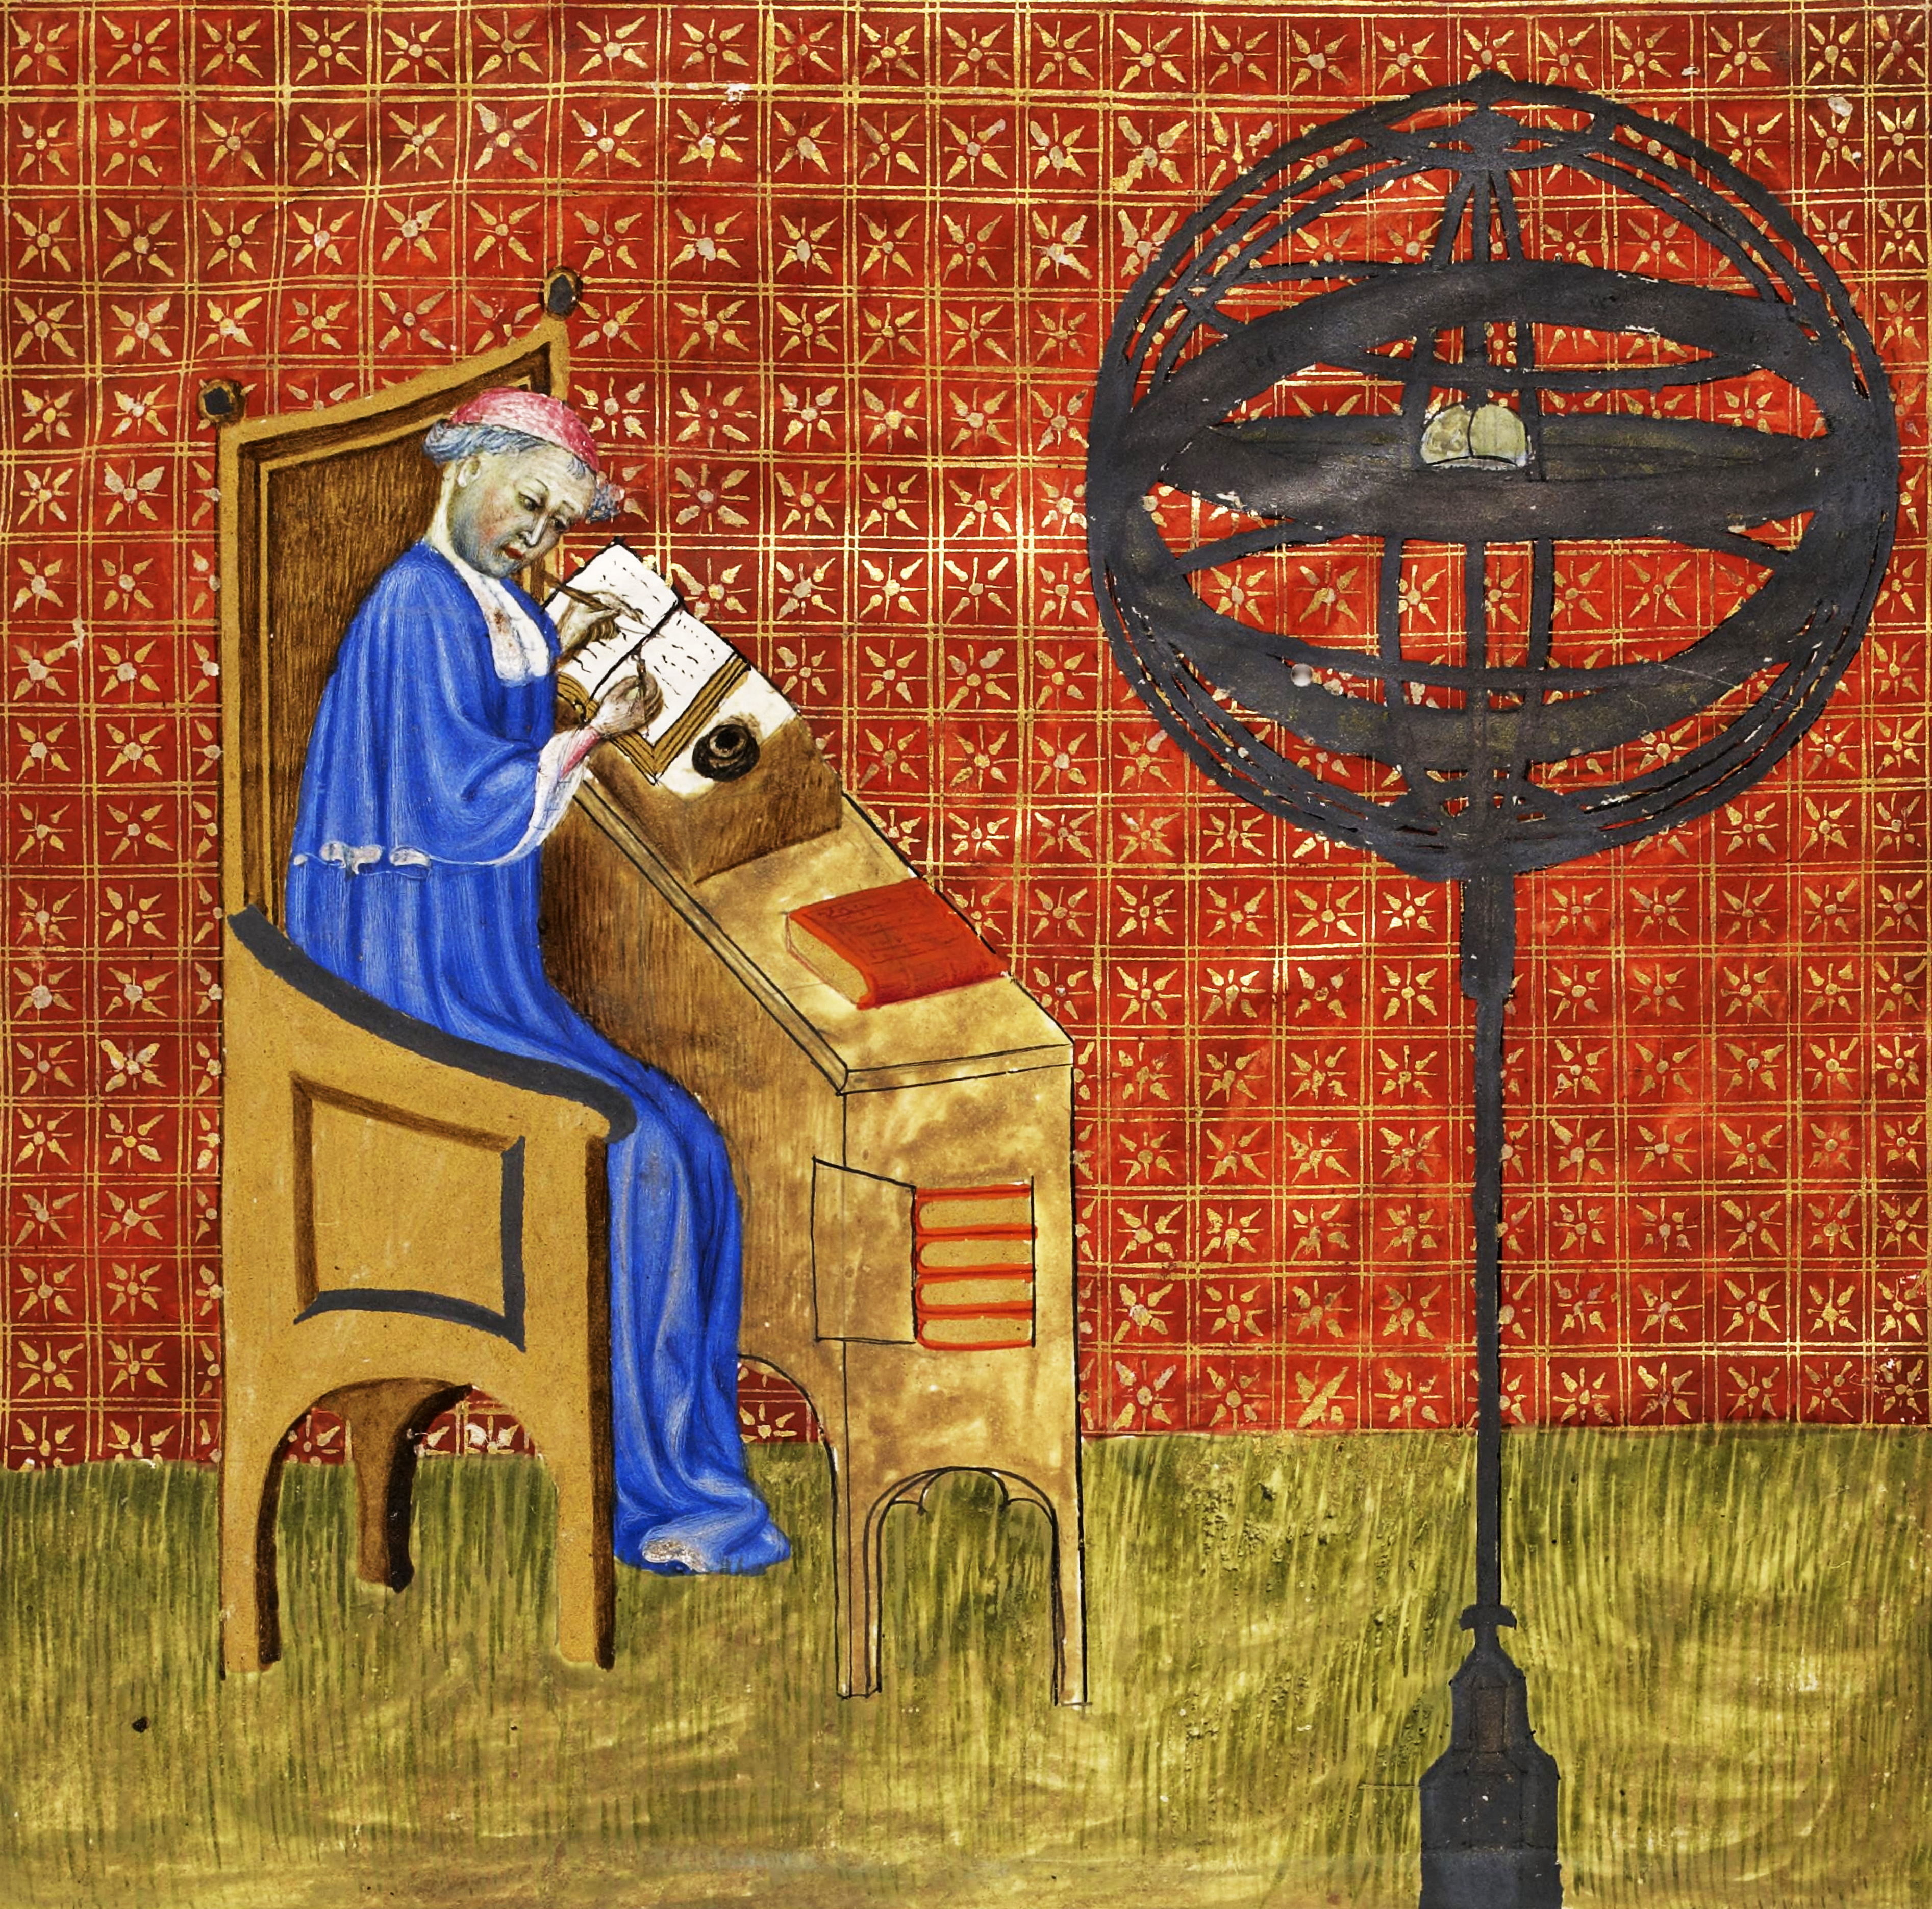
\includegraphics[scale=.25]{a20111203MentalDeath-img001.jpg}
\end{wrapfigure}
Gornahoor places the fateful junction of Western intellectual history at Francis Bacon\footnote{See Section~\ref{sec:BaconModernity} in this book.}. It was Bacon's head-on assault against metaphysical knowledge (``useless knowledge'' that is not power) which signaled Western intention to abandon the medieval project wholesale. Although at various times and places, other movements had been made, Bacon's \emph{New Atlantis} was more completely ``modern''\footnote{\url{http://plato.stanford.edu/entries/francis-bacon/}} and also more suited to corrupt its age. Bacon (for instance) uses ``Magic'' to refer to applied science \& technology, while ``Knowledge'' becomes essentially what we mean today as ``Science''. Blake's ``dark, Satanic mills'' were seen, prophecied, \& invoked by Bacon, and in their present form. Other ``seers'' had conjured up similar forms, but Bacon was seminally specific. Bacon's project (for instance) is innately inherent in William of Ockham's denial of universals. Richard Weaver writes\footnote{\url{http://www.nyx.net/~kbanker/chautauqua/consequences.html}}:

\begin{quotationx}
Surely we are justified in saying of our time: If you seek the monument to our folly, look about you. In our own day we have seen cities obliterated and ancient faiths stricken. We may well ask, in the words of Matthew, whether we are not faced with ``great tribulation, such as was not since the beginning of the world.'' We have for many years moved with a brash confidence that man had achieved a position of independence which rendered the ancient restraints needless. Now, in the first half of the twentieth century, at the height of modern progress, we behold unprecedented outbreaks of hatred and violence; we have seen whole nations desolated by war and turned into penal camps by their conquerors; we find half of mankind looking upon the other half as criminal. Everywhere occur symptoms of mass psychosis. Most portentous of all, there appear diverging bases of value, so that our single planetary globe is mocked by worlds of different understanding. These signs of disintegration arouse fear, and fear leads to desperate unilateral efforts toward survival, which only forward the process.

Like Macbeth, Western man made an evil decision, which has become the efficient and final cause of other evil decisions. Have we forgotten our encounter with the witches on the heath? It occurred in the late fourteenth century, and what the witches said to the protagonist of this drama was that man could realize himself more fully if he would only abandon his belief in the existence of transcendentals. The powers of darkness were working subtly, as always, and they couched this proposition in the seemingly innocent form of an attack upon universals. The defeat of logical realism in the great medieval debate was the crucial event in the history of Western culture; from this flowed those acts which issue now in modern decadence.

One may be accused here of oversimplifying the historical process, but I take the view that the conscious policies of men and governments are not mere rationalizations of what has been brought about by unaccountable forces. They are rather deductions from our most basic ideas of human destiny, and they have a great, though not unobstructed, power to determine out course.

For this reason I turn to William of Occam as the best representative of a change which came over man's conception of reality at this historic juncture. It was William of Occam who propounded the fateful doctrine of nominalism, which denies that universals have a real existence. His triumph tended to leave universal terms mere names serving our convenience. The issue ultimately involved is whether there is a source of truth higher than, and independent of, man; and the answer to the question is decisive for one's view of the nature and destiny of humankind. The practical result of nominalist philosophy is to banish the reality which is perceived by the intellect and to posit as reality that which is perceived by the senses. With this change in the affirmation of what is real,, the whole orientation of culture takes a turn, and we are on the road to modern empiricism.
\end{quotationx}

Conservatives quote Weaver all the time, but nobody takes this seminal passage seriously (or indeed, seems to have read him attentively at all). George Heart in \emph{Dogmatic Faith \& Gnostic Vivifying Knowledge} actually suggests that Aquinas represents a ``first compromise'' by way of Aristotle's influence. Although Hylomorphism is a far cry from modern empiricism, it was a first step:

\begin{quotex}
Although Albertus Magnus himself started to work at amending Aristotle's most conspicuous aberrations, he could never bring his work to completion, and he left the rest of that impossible task to his disciple Thomas Aquinas. We say ``impossible'' because we fully know now that Plato and his unfaithful disciple who betrayed his teachings after having spent 20 years in the Academy could never be reconciled. Origen was right when he said that Aristotle was simply a traitor.

\end{quotex}
Heart thinks that Aquinas betrayed Aristotle to attempt to synthesize Plato \& his wayward student, but others were not so discriminating; Catholics should not forget that in 1210, the Church found it necessary to issue a condemnation of indiscriminate use of Aristotle, Averroes, and Avicenna. The threat from combining things that ought not to be combined was ``sterile heterogeneity'', such as can be found in St. Anselm (1033-1109).

As GK Chesterton noted\footnote{\url{http://distributistreview.com/mag/2011/12/two-difficulties/}}, the big task (exoterically) of our present generation is to conduct committees of correspondence in order to lay the groundwork for understanding what was lost, and why. A scope for action is very limited, but this is to simply put us in the same position as those who created the avenues of decay all those centuries ago – we will be forced to rethink: a man in prison has time for reflection, at last.



\flrightit{Posted on 2011-12-03 by Logres }

\begin{center}* * *\end{center}

\begin{footnotesize}\begin{sffamily}



\texttt{Michael on 2011-12-03 at 14:59 said: }

Outstanding post. What authors do you recommend to start us on the task?


\hfill

\texttt{Logres on 2011-12-04 at 00:41 said: }

Well, one has to remember that the ``Greater Struggle''

\url{http://www.gornahoor.net/?p=3005}

takes precedence, even for the fighter or the peasant, whomever they are. Because of this, Tomberg's book has to be a good place to begin the arts of transformation of the self; Tomberg represents a continuation of the Inkling's insight that the moral universe is opened by the imagination – that is, it is a key, because it lets us out of the modern prison. But it isn't an end in and of itself, contra the poets. I would suggest that a Westerner include a certain familiarity with the enemy – even Orthodox monks in America study Nietzsche, if for nothing else than to help ``see through'' flimsy arguments supposedly made on that very basis. It would be interesting to know (for instance) where Bacon got his ideas (that was discussed a little on that post). Beyond that, I would say ANY book that helps recover the link between Christendom and the Greco-Roman/Nordic heritage is a priceless asset, and in this sense, it hardly matters where one starts. For those who are contemplative, Augustine's Confessions or Boethius' Consolation (my favorite). The dialogues of Plato are read by very few people, and Platonism is a strong antidote to nominalism/empiricism in all its forms. It teaches good mental hygiene. Any historical work that recasts the data into an unfamiliar but plausible shape (eg., Polyani's Great Transformation which debunks the golden mythos of modern capitalism to a great degree) can be useful for purging mental parasites that swarm around us on the TV, in the papers, etc. Anything to set the mind to actually ask itself questions and answer is useful. The turning point for me was realizing how bad the Reformation was, in so many ways:

\url{http://jcrao.freeshell.org/LouisVeuillotReevaluation.html}

Tarapelli is another good Catholic political writer, as is Cortes.

Sir John Polkinghorne has done some thoughtful writing on the implications of quantum physics for religion, and vice versa, although he is not a ``traditionalist'' – he is, however, an independent thinker and someone who actually ``counted'' in the history of physics. It depends upon your field of interest, your temperament, and whether you want to be a scholar, a man of letters, or a fighter. Dante's political treatise on De Monarchia is reliably good, I've been told. And there is a whole slew of new scholarly works, compilations, editions, etc. out there, such as Glenn Magee's new study on Hegel \& Hermeticism, which places an old Leftist favorite in a brand new light. We have to transmute, or undo, what has been done. Perhaps someone should study Bacon and trace how and where he got his concepts and twisted them, in what ways and by what means they shadow and parody truth. They wouldn't be so powerful unless they contained some measure of the truth, even to be powerful in the debased way they are. Remember what Cologero has quoted before – ``the errors of the great are more interesting than the rightness of the small''. Alchemy is important because I think that is what modern science parodies, or apes. Someone could do worse than begin to follow in Franz Bardon's footsteps, and read what he wrote about the Kabbalah, etc. But beyond that, any book which ``calls'' to you in your personal quest for truth, your hunger to escape the prison, is going to help you, by inexorable laws, even if negatively. Following footnotes can sometimes lead you in that quest. If you are specifically interested in Science \& Religion's interaction, I can be more specific. Or if you tell me anything more of where you're coming, I can also be a little more specific. Personally, I need to read Evola on the Grail and his work on magic. I also need to finish Tomberg's Meditations, which are fabulous. What are your favorite books, and what is your ``read before I die'' list?


\hfill

\texttt{Charlotte Cowell on 2011-12-04 at 12:36 said: }

I also love MoTT, it's far and away my most well-used book. I also love Sufi poetry – Bird Parliament, Rumi and the Rubaiyat of Omar Khayyam – and of course The Prophet by Khalil Gibran is a magical masterwork that even a child could read. The Master and Margarita is probably by favourite novel and Carlos Castaneda inspired me to become conscious in dreams. Whether fact or fiction, his journeys with Don Juan certainly fire the imagination. A Midsummer Night's Dream is my favourite Shakespeare play (or Bacon play as some of you probaby think!) and Yeats is one of my favourite poets. Von Balthasar's Prayer is one of the best tools for helping one to learn contemplative prayer that I know of and certain parts of Augustine's confessions have touched me very deeply and 2 Corinthians 6 is my favourite part of the Bible. From the Greeks I love the dramas and Orphic Hymns. More recently The Discovery of Heaven by Harry Mulisch is amazing (as is the film of the same name), but the best thing I ever EVER read in my life was a love poem written by God for the lost Divine feminine which generated the universe so he could try to find her :-)


\hfill

\texttt{logres on 2011-12-04 at 17:08 said: }

Charlotte, what do you mean, conscious in dreams? Waking up inside of them?


\hfill

\texttt{logres on 2011-12-04 at 17:11 said: }

I should also say that Chesterton and Belloc thought (think) that those who can, should go back to the land, in one way or the other. This gives an existential, practical base to the struggle which permits more independence of thought, than (say) someone whose opinions (if known) could affect their employment. Evola is still the best Western introduction for many people, I would think? Gornahoor has a lot of his essays here – the one on Falangism is good, as well as Reincarnation.


\hfill

\texttt{nous on 2011-12-04 at 17:12 said: }

Placing the cosmos in philosophical terms represents the first fall or any dialectics that could elicit an opposite reaction, outside even of historiography. Somewhere at the point of paradisaical origins authority was over-ruled. But let me echo Micheals question: ``Moar sauce.''

Indeed, I commend you Logres on those examples given but what of the action orientated spirit? What recommendations can be given to those who wish to follow a direct path of the fighter (striking both inner and greater battles). I would like you or any member of the Gornahoor staff to address this important question.

I have read Franz Bardons books(achieving the goals therein if even possible beyond the 4th level is another question). Evola's operative methods in ``Introduction to Magic'' and ``Yoga of Power'' are intriguing but not final. Catholicisms mortification of the flesh is another tempting facet, as is that of the Buddhist/Zen response to ``no mind'' and to the perfection of ones actions. What is needed is real life engagement which is what I believe O.D founder St Jose-maria Escriva had in mind to the inter-war period of decadence he found himself in.


\hfill

\texttt{Charlotte Cowell on 2011-12-04 at 19:27 said: }

Yes, Don Juan's teaching to Carlos about dreaming, is in fact a useful method for learning how to `wake up’ – to become conscious with will and mind – in a dream. The Indian tells his pupil he must strive to see his own hands in a dream, which takes the pupil a long time. It took me ten years, although I had out of body experiences often, in both the lower and higher astral, but not of my own volition until this one time. Basically one conditions one's self to associate seeing the hands with being conscious, it's a form of inner programming. Actually one could choose anything, it's the technique that's important in this case rather than the particular, as I understand it. One might equally decide to see one's feet I suppose. When this happened to me (ie, I saw my hands), firstly I note they looked very strange to me, being whiteish grey and translucent in that state it led to the vision of Genesis I mentioned above: 

\url{http://alchemical-weddings.com/alchemical-weddings/tunnel-vision}

\url{http://alchemical-weddings.com/alchemical-weddings/rainbow}

more generally, the shamanic training helps to hone the faculties necessary for fruitful spiritual work, such as concentration, self discipline, dedicated endeavour, right motivation, discernment etc.


\hfill

\texttt{Charlotte Cowell on 2011-12-04 at 19:31 said: }

I agree with Chesterton and Belloc by the way, that's why I'm off to Guatemala in February to build a house, farm the land, keep bees etc….

\url{http://www.greennewworld.org/}

it's the only way forward unless we want Earth to become an inorganic sort of hell with half human half robots, weird animal hybrids, totally polluted environments etc. It'll happen sooner than people think if there isn't a significant mass turnaround in terms of commitment to saving the world


\hfill

\texttt{logres on 2011-12-05 at 19:06 said: }

I think I may defer to Cologero on your question, Nous (and Michael, if there was more). My path is intellectual fighting, when it comes to initiative. It is difficult for me to recommend ``when'' or ``how'' unless it is already clear. You are essentially ( I think) wanting an order, something that will require special gifts to institute. If I was going to recommend something, Coudreanu's Legion of the Archangel Michael might be a good place to start. It would be interesting to examine this movement in a dispassionate sense, and to parallel this study with more research along Evola's lines. I am not qualified to state anything further.


\hfill

\texttt{logres on 2011-12-05 at 23:04 said: }

I hate adding to my essay, but I should devote something to this man:

\url{http://truerestoration.blogspot.com/2008/10/book-review-liberal-illusion-by-louis.html}

I don't think any effective rebuilding can occur until the insights of Christian theology are yoked with metaphysical insight (which necessarily draws on pagan elements). Essentially, as Charlotte has pointed out, this is a matter of connecting dots in every sense of the word, which is Cologero's ambitious and noble project. If Catholic dogma could be transmuted/translated into metaphysics, and vice versa, by an elite, then the path of the fighter is made much easier, and less subject to disastrous mistakes as they struggle to bore back into their heritage from the outside. So long as one individual ``hears the music'' and does not bow the knee to Baal or any lesser gods, the world exists for him/her. That being would be sovereign. Like a soul who battles to save the body, or a spirit, the soul, so would that one person fight to inherit the world called earth for the Pantocrator. They would be the viceroy.


\hfill

\texttt{Charlotte Cowell on 2011-12-06 at 06:09 said: }

Yes, we have to know where we came from to really know where we're going – the past proceeds from the future as much as the future proceeds from the past. When I was first converted to Christianity I discovered a sublime unity – and no conflict – with classical religion, but also Buddhist and Sufi principles in a truly universal sense. Problems might come via the reincarnation doctrine, which might cause one to redevelop a soul attachment to the `old ways'. then trauma when this is necessarily severed. However consciousness of the hows and why helps make this easier to bear and it is not so difficult to put those kinds of memories back into the realm of imagination.


\hfill

\texttt{Gabe Ruth on 2011-12-06 at 10:10 said: }

Thanks for this, it really got my blood racing. For those more action oriented, John Robb (writes Global Guerrillas) is very interesting and somewhat practical. Though I've never seen him comment on metaphysics himself (has linked to others of this bent on occasion), his thoughts on how far wrong we have gone and where we need to go jive with the ideas around here with regards to worldly steps. The whole resilient community is worth a look, though they are generally not cognizant of metaphysics.


\hfill

\texttt{logres on 2011-12-06 at 22:37 said: }

That's a good point about ``time flowing backwards''.


\hfill

\texttt{logres on 2011-12-06 at 22:38 said: }

I've heard of John Robb, \& will look him up, thank you.


\hfill

\texttt{Perennial on 2011-12-08 at 03:51 said: }

I recommend anything on the Action Francaise, which works were so action-packed I became a traditionalist just from reading a history of it! The Camelots du Roi, their seminars, their newspaper and of course the pivotal Charles Maurras were all inspirational. The Legion is excellent also, and of course anything related to the Carlists of Spain is great, although I know of only 2 works in English. These were all action-based movements (Action Francaise says it all) and therefore an excellent study for those who wish to benefit from them as well as to attempt to rectify their shortcomings.


\hfill

\texttt{Charlotte Cowell on 2011-12-08 at 14:58 said: }

`If Catholic dogma could be transmuted/translated into metaphysics'

Does Rudolf Steiner go some way towards achieving this? Granted he is elliptical and strange, but he was pretty ahead of his time all the same….

Apart from that, I think this is a matter that is wholly dependent upon subjective experience, because without that one would not necessarily recognise the analogies in philosophical/theological works. Even then it depends on `right place and right time'. I might read something one day that means nothing, but ten years later speaks volumes (or indeed vice versa). 

In terms of a catholic theologian who regularly speaks volumes, von Balthasar I find outstanding. Recently this aphorism from his `A grain of wheat'. helped me to understand a very particular spiritual `problem' or `question' I had pertaining to one experience in particular that was both very upsetting and something for which i felt unaccountably (but profoundly) grateful. At the time I viewed it as being a certain spiritual death, so the gratitude was difficult for me to comprehend, although I did at the same time `see' something akin to fireworks going off deep in outer space so assumed it was an occasion for some form of celebration. The extract is on my blog (it is short):

\url{http://alchemical-weddings.com/alchemical-weddings/integration}


\hfill

\texttt{logres on 2011-12-08 at 23:52 said: }

Charlotte, here is a quote from what you posted:

``But if no understanding is developed, if this particular faculty is stamped out, if those who speak about faculties of this kind are put away as if they were insane, disaster in inevitable and humanity will sink in the morass of materialism. Everything will depend upon whether understanding is awakened for Spiritual Science, or whether Ahriman will succeed in suppressing its intentions…''

I've linked to Bondarev's interpretation of Steiner, which removes some of the necessary detritus and evolutionary Zeitgeist which adheres to Steiner's work (which Cologero has quite properly drawn attention to). This is almost a quote of St. Anthony – ``in that time, when men go mad, they will find him who is not mad, and call him mad''. Isn't this where we have arrived at? Even Phillip Rieff (a total ``secularist'' \& Jew) could see this quite clearly. Goethe also prophecied it – ``we will all take care of each other in hospitals''. The stench of the mental sick bed is all around us. But I think Steiner is a piece of the puzzle, provided someone can interpret him in a less ``spiritualist'' viewpoint, although the ``spiritualist'' viewpoint had more traditional elements, then. So I think this is right, your insight here.


\hfill

\texttt{Charlotte Cowell on 2011-12-09 at 05:37 said: }

In answer to this question:

``in that time, when men go mad, they will find him who is not mad, and call him mad''. Isn't this where we have arrived at?''

No, I think we have just been there and that now the network of the `non mad’ – ie, the pioneers – have collectively `fought off' the assault, so to speak, and have consolidated their forces. Just. It's very early days but we're on the way back up now because a critcal mass of `seers and believers' has been reached. Only just! it's inconceivable that once the universal tipping point has been reached we'll collectively fall back into the abyss – we went through the abyss to ensure we won't go there again en masse. 

Metaphorically speaking, enormous numbers of people are loaded onto the `Mother Ship' ready for take off, mostly without realising it!

I do think, however, that perhaps more than ever these are days for prayer and focus on the joyful and luminous mysteries.


\hfill

\texttt{Charlotte Cowell on 2011-12-09 at 05:41 said: }

By the way I am not a diehard fan of Steiner – I agree with many of the well known reservations – it's just that I can see that he could see and am only recently starting to understand how he presented his information. He relentlessly spoke to the developing spiritualised being in us all and was fearless in risking being wrong in order to be right! Crazy wisdom….


\hfill

\texttt{Boreas on 2011-12-09 at 08:35 said: }

Charlotte, I think you are right about the fact that ``a critical mass of seers and believers'' has been reached and we're heading towards a new upward pointing cycle in the longer run, but despite – and because of! – this, the current world-age is in its death throes and the world is on the verge of a third planetary cataclysm in the short run. No utterance for world peace etc. can change this fact, no matter how good-willed a man or a woman might be. (I think you know this also and this was not exactly what you were referring to, but as an semi-official voice of cosmic pessimism I had to say this!)

Here's the true ``beef'' of the matter: this is not a call for panic, anguish and despair, but for hope and joy. Things couldn't be otherwise than they are. The divine spirit of man is awakening again from its slumber and THIS is the very thing that is the primal cause of all that's happening – even in its negative manifestations.


\hfill

\texttt{Charlotte Cowell on 2011-12-09 at 09:12 said: }

Boreas yes, I think we are in agreement and I am in the mode now of being positive. I stared into the abyss from 2009 – 10 and at the time I wondered how people would cope with what was to come, if it proved so devastating to me personally, for all my faith and hope in `other things'. Clearly we are in a time of major, enormous change – an `anything goes' type of situation in which all the birds are coming home to roost. The relief comes from the fact that karma is finally being faced, because as you point out, we can't move on with the new until we've moved on from the old. However I don't see that there is a need to throw the baby out with the bathwater, and we should always bear in mind that the heavenly quality of mercy `wins' in the end. This is why prayer is still so important. I firmly believe that we should all be praying for mercy and redemption – for both self and others – on a daily basis now, as to do less would be to deny the possibility of damage limitation. Anything is possible.

There is something on my blog here about Prayer/Benediction:

\url{http://alchemical-weddings.com/alchemical-weddings/act-of-benediction}


\hfill

\texttt{Charlotte Cowell on 2011-12-09 at 09:31 said: }

\url{http://beforeitsnews.com/story/1483/117/Pope\_Highlights\_Marys\_Role\_As\_Woman\_Of\_The\_Apocalypse.html}


\hfill

\texttt{Boreas on 2011-12-10 at 10:45 said: }

You are of course right Charlotte. I never meant to mean that prayer is futile or hoping for a peaceful solution to world problems is in vain / naïve. On the contrary, I think these are the very duties of spiritual or religious people in these times.


\hfill

\texttt{Golgonooza on 2011-12-12 at 12:04 said: }

Thanks for the post, especially the link to the Richard Weaver writing, which was fascinating. Thanks also Charlotte, for the Von Balthasar aphorism; as usual you have brought something to my awareness which chimes with what I'm currently pondering!


\end{sffamily}\end{footnotesize}

\section{Perspectivism}

\begin{quotex}
It seems to me important that one should get rid of the All, the unity, some force, something unconditioned; otherwise one will never cease regarding it as the highest court of appeal and baptizing it `God'. One must shatter the all; unlearn respect for the all.

\end{quotex}
Some definitions:

\begin{description}
\item[Naïve Realism ]

The view that reality is ``out there, right now" and that knowing is like ``seeing" (see Bernard Lonergan, \emph{Insight}). This is probably the view of the average unreflecting person. However, it is difficult to defend philosophically. 

\item[Correspondence Theory of Truth ]

The idea that truth consists of statements that ``correspond" to reality ``out there". Naïve realists usually believe this, though some philosophers accept it, too (e.g., the logical positivists). In this case knowledge is equivalent to a collection of true statements. The philosopher Alvin Plantinga describes the omniscience of God to be: ``He believes all true statements and doesn't believe any false statements." This assumes that all Truth can be expressed verbally. 

\item[Perspectivism ]

Nietzsche's position regarding truth, which asserts that there is no such thing as an absolute truth, but merely different perspectives that one can adopt. We could think of truth as a sculpture, where there is no single ``right" perspective to look at it. To properly appreciate the sculpture, we must walk around it, looking at it from as many different perspectives as possible. Similarly, Nietzsche insists that we should not get caught up in dogmatism, but rather look at the truth from as many perspectives as possible. 

\end{description}
Of course, Tradition denies the validity of Naïve Realism, the Correspondence Theory and Perspectivism, for a few reasons.

\begin{enumerate}
\item Against naïve realism – the objection is that appearances are deceptive (Maya) and reality is best understood as the source of the appearances. This source is beyond all appearances. 
\item Against the correspondence theory – this theory assumes that all truth can be known/expressed by the rational mind. However, Tradition has always insisted that there is a knowing (gnosis, jnana) higher and more certain than the rational mind. This is clear from the Eastern Traditions. However, it used to be true even in the West. The Medieval Scholastics distinguished between the intellect and the rational mind (although they are mere synonyms today). Or they insisted that faith (which again meant something different from what it means today) is a higher truth than the rational mind. The intellect is associated with the heart — on certain French cathedrals, there are statues of headless saints holding their heads in front of their hearts (the legend of St Denis) — this symbolizes the subservience of the rational mind (head) to the intellect (heart). 
\item Against perspectivism – that's precisely the point: ultimate truth cannot be known from the phenomenal world, no matter how extensive the experience (i.e., number of perspectives). One is left only with appearances, or mere opinion. Truth can only be know by transcending the phenomenal world. This is brought out most clearly by Nagarjuna in Madhamyka Buddhism (see Murti: \emph{The Central Philosophy of Buddhism}). 
\end{enumerate}
The Traditional teaching is that the phenomenal world of appearances is always changing, and so cannot be the ultimately Real. From observing the arising in consciousness of the phenomenal world, one discerns the one constant is consciousness itself. In that sense it is unchanging, since it is present in every act of consciousness, yet is not itself a part of the phenomenal world. It is also without quality – i.e., it has no color, weight, taste, etc, but is rather the source of all qualities. In that sense it is the most real – and this is the common understanding of the real as the (hidden) underlying source of what only appears to be going on.


\hfill

Originally, class notes for a seminar delivered in 2004.



\flrightit{Posted on 2011-02-23 by Cologero }

\section{Pinker the Thinker}

\begin{quotex}
So, how many people know how to observe? And of these few, how many to observe themselves? `Everyone is farthest from himself’ — every person who is expert at scrutinizing the inner life of others knows this to his own chagrin; and the saying, `Know thyself'. addressed to human beings by a god, is near to malicious. \flright{\textsc{Friedrich Nietzsche}, \emph{The Gay Science} §335}

\end{quotex}
The NY times published an article about a year ago on \textit{Why the Fight Over Abortion Is Unrelenting}\footnote{\url{https://www.nytimes.com/2019/05/29/opinion/abortion-restrictions-politics.html}}. The answer is postulated in the first paragraph:

\begin{quotex}
Why is the debate so bitter, so emotional? Part of the answer is very simple: the two sides share almost no common premises and very little common language. 

\end{quotex}
Our intent, therefore, is not to debate the morality or legality of abortion, but to explore the lack of common premises and language. Nevertheless, prior to 1973, there was a long stretch of time in which there were common premises around the morality and legality of abortion. In any case, whatever changes in attitude have occurred in recent decades, the positive law cannot exceed the general moral level of the population.\footnote{\url{https://gornahoor.net/?p=8578}}

Since Steven Pinker is a well-respected public intellectual today, we want to focus on his contributions to the discussion.

\paragraph{Health}
\begin{quotex}
Health is the state of an organism in which disease and infirmity are absent. In particular, fertility is considered to be the healthy state and infertility is the inability of a person, animal or plant to reproduce by natural means. It is not the natural state of a healthy adult, except notably among certain eusocial species (mostly haplodiploid insects). (\emph{Wikipedia}) 

\end{quotex}
So apart from some insects, infertility is not the natural state of a healthy adult. Hence, artificial means to prevent the healthy state of fertility needs to be justified, not the other way around. Of course, the Times article will justify them because there may be other health concerns beyond fertility in play. Moreover, throughout history the prevention and termination of births was quite unreliable. Now that medicine has transformed that process, attitudes have changed: demonstrating once again that the material conditions of life alter consciousness.

\paragraph{Life}
The pro-life cause has not helped with the common language, due to its insistence of referring to the unborn as a baby or child. Nevertheless, for those who effing love science, the unborn is scientifically a human life. It starts as an embryo, then becomes a fetus. So a human life, in the biological sense, passes through multiple stages: embryo, fetus, infancy, childhood, adolescence, etc. That is the starting point for a common language.

The other mistake is to equate abortion with murder. Legally, there are different crimes associated with the loss of a human life by another human, depending on circumstances. Hence, abortion should have its own legal category, unless you are ready and willing to execute mothers, doctors, nurses, etc. In an earlier article, Pinker makes this point:

\begin{quotex}
Mothers who kill their newborn infants should not be judged as harshly as people who take human life in its later stages because newborn infants are not persons in the full sense of the word, and therefore do not enjoy a right to life. Who says that life begins at birth? 

\end{quotex}
Pinker is using rather loose language here by confounding the notions of personhood and life. Life is a scientific category and begins long before birth. Personhood is a metaphysical category, which leads to the next topic.

\paragraph{The Right to Life}
Once again from Pinker:

\begin{quotex}
To a biologist, birth is as arbitrary a milestone as any other. No, the right to life must come, the moral philosophers say, from morally significant traits that we humans happen to possess. One such trait is having a unique sequence of experiences that defines us as individuals and connects us to other people. Other traits include an ability to reflect upon ourselves as a continuous locus of consciousness, to form and savor plans for the future, to dread death and to express the choice not to die. And there's the rub: our immature neonates don't possess these traits any more than mice do. 

\end{quotex}
Well that is too bad for the biologists who cannot tell with certainty what life is, thereby destroying its claim to be a serious science. What Pinker is actually asserting is the ``right to life" — which depends on being a person — and not really when biological life begins. However, his definition of ``person" is arbitrary, and not at all scientific for someone who claims to be a scientist.

By the way, mice do dread death which should be common knowledge.

\paragraph{The Will to Life}
The \emph{Declaration of Independence} correctly asserts that the right to life comes from God, not from the state or the arbitrary opinions of so-called ``moral philosophers", politicians, talking heads, etc. Every living being derives that right from its own Will to Life.

Life is being discovered in the most unlikely and seemingly inhospitable environments. In every little crack in asphalt or concrete, you will probably find some plant trying to poke through it. Even around Chernobyl, which is unsuitable for human habitation, an entire ecosystem of flora and fauna has been thriving there.

A life is never a ``clump of cells" because it has a central organizing principle. That makes it a life rather than an arbitrary clump. A human artifact, on the other hand, lacks its own organizing principle; it may seem to function as a unit, but that is because its apparent unity is actually inserted by the designer.

The conclusion is that a life has value in itself, not because it may or may not have a value to others.

\paragraph{Genetic Health}
Pinker provides the evolutionary explanation for opposition to abortion:

\begin{quotex}
[It] is straightforward. Humans are unusual among mammals in that men invest in their children, feeding, protecting and teaching them. As a result, a father who invests in his children will have more successful children, which favors any genes that tilt a man toward investing in his children. But of course that only works if they are his children. Evolutionarily speaking, cuckoldry is the worst thing that can happen to a man, because his investment would be wasted in protecting another man's genes. 

\end{quotex}
So Pinker confirms that opposition to abortion is a sign of a healthy genetic makeup. That is, the selfish gene expresses its impulse to pass on and preserve itself. The obvious corollary is that abortion is, from the biological point of view, akin to a deleterious genetic mutation. The genetic urge to perpetuate oneself is so strong that it controls our mental processes. Pinker asserts, without providing any evidence:

\begin{quotex}
the actual thoughts and emotions running through people's brains are not about babies, cuckoldry, genes, investment or any of the concepts that enter into the ultimate, long-term, evolutionary explanation of people's motives. 

\end{quotex}
I don't see how our genes become aware of complex social and political issues, even to the point of controlling thoughts. Certainly Pinker does not demonstrate a causal chain. If anyone other than Pinker had said that, he would be considered a crank. Note how the Times sneakily alters Pinker's point:

\begin{quotex}
The \emph{men} who are pressing to make abortion illegal are unaware of the evolutionary forces motivating them 

\end{quotex}
Pinker said that ``\emph{people}" are unaware, unless the Times is using ``men" in the generic sense to apply to human beings generally, without regard to sex. But I don't think so.

By this logic, unfortunately, the promotion of abortion must be the sign of a deleterious genetic mutation, since the genes of those people fail to get passed on. Moreover, the desires of ``people" to pass on their genes, and \emph{to not pay for the upbringing of other men's children}, must be indicators of biological health. If an evolutionary psychologist can show otherwise, perhaps he should give it a try.

Of course, there may be moral reasons that transcend biology, but then we are leaving the realm of science.

\paragraph{Group Consequences}
\begin{quotex}
A country whose population is stagnating, diminishing, or aging, creates a vacuum for younger, more active, poorer peoples. A country that no longer has children is a country that has lost confidence in itself, its culture, its history and its values. \flright{\textsc{Fr. Gregory Celier}}

\end{quotex}
Decisions that seem best for an individual often have adverse effects on society as a whole. Artificial contraception is an example. It seems so reasonable to gain the pleasures of sexual intercourse without the possibility of an unwanted pregnancy; the alternative seems absurd to most people today. \emph{Humanae Vitae} warned of the long-term consequences, including the decline of moral standards. Another consequence is the reversal of the general understanding of the purpose of sex.

Moreover, when individual decisions are repeated, the social consequence is the decline in the general population. Most European countries have a sub-replacement level birth rate, as individuals deliberately choose not to reproduce. The social upheaval that will result from this will be ongoing. Nevertheless, the individual does not, and cannot, take the societal consequences into consideration.

\paragraph{Anti-Life}
\begin{quotex}
To the woman he said: in sorrow shalt thou bring forth children \flright{\textsc{Genesis 3:16}}

\end{quotex}
When the purpose of sexual activity is pleasure alone rather than reproduction, then pregnancy is no longer understood as an indicator of health, but as a curse to be avoided. The following is a tweet that had more than 50 thousand ``likes", the last time I checked.

\begin{quotex}
WHY IS GIVING BIRTH SO NORMALIZED??? LIKE YOU LITERALLY CARRY A MONSTER INSIDE YOU THAT MAKES U HORMONAL FOR 9 MONTHS THEN SPLIT YOUR BODY IN HALF GIVING BIRTH?? AND LIKE PEOPLE JUST EXPECT THAT OF WOMEN????????!!!!! 

\end{quotex}
This young woman understands Eve's curse, probably better than most. Woman's sex drive is so strong in order to overcome that reluctance to pregnancy. In most if not all materially advanced countries, the birth rate is becoming precipitously low.

\paragraph{The Best Life}
Several months ago, USA Congresswoman Katie Hill resigned after a photograph appeared of her grooming a staffer while naked. She admitted to being bisexual and engaging in three-way relationships. Surprisingly, her own party coerced her to resign.

That evening, I watched a liberal commentator on TV who condemned the resignation. She defended Mrs. Hill with the interesting claim, ``all she was trying to do was to live her \textbf{best life}."

I was taken aback because I had never considered a life of sexual excess and drug use as anyone's ``Best Life". Traditionally, the best life has been considered a life of virtue. Now there may be disputes about the precise virtues, but they have been close enough. Katie Hill's lifestyle would never qualify.

\paragraph{Death and Violence}
One often hears, ``Violence is never the solution." Obviously, that is quite untrue. Violence ends wars, stops criminals, overturns government, provides food. A youthful unwanted pregnancy more likely than not might prevent the woman from her ``best life", however understood. Perhaps she would drop out of law school, or give up dreams of Hollywood stardom. Or she could terminate the pregnancy and get her life back on track.

When it is a matter of convenience or adherence to abstract principles, convenience will usually win out.

\paragraph{Summary}
The lack of common premises and languages have been delineated. One side is arbitrary in its understanding of life, genetics, physical health, pleasure, convenience. The other side is objective in its understanding of life, health, the purpose of life.



\flrightit{Posted on 2020-06-03 by Cologero }

\begin{center}* * *\end{center}

\begin{footnotesize}\begin{sffamily}



\texttt{Tannheuser on 2020-06-05 at 12:15 said: }

I've always felt that ``Abortion is murder" was a cheap and inaccurate talking point. Again there seems to be no distinction between ``human" (biological entity) and a ``person" (a metaphysical category as you point out), which causes a lot of confusion on both sides. Canto XXV from Dante's Purgatorio is relevant here. The below makes a lot more sense intuitively than the ideas in vogue today:

Having become a soul (much like a plant,

though with this difference—a plant's complete,

whereas a fetus still is journeying),

the active virtue labors, so the fetus

may move and feel, like a sea-sponge; and then

it starts to organize the powers it's seeded.

Open your heart to truth we now have reached

and know that, once the brain's articulation

within the fetus has attained perfection,

then the First Mover turns toward it with joy

on seeing so much art in nature and

breathes into it new spirit—vigorous—

which draws all that is active in the fetus

into its substance and becomes one soul

that lives and feels and has self-consciousness.


\end{sffamily}\end{footnotesize}

\section{Prelest and Other Dreams}

By now, everyone should have figured out the meaning of my dream, which is:

\begin{quotex}
\emph{Sleeping people are full of spiritual delusions. Awake men are more cautious.} 

\end{quotex}
This spiritual delusion is called \emph{prelest}. This cannot be considered a rare condition, but rather it is the universal state of people. It begins with a false thought. Since the nature of error is not to recognize itself as error, a whole worldview is weaved from that thought and all its consequences. Then, one's very identity becomes associated with that worldview, to the extent that any challenge to the worldview is taken as a personal threat. That is why people become so enraged and irrational when discussing or debating worldviews. The alternatives, as in every menace to one's life, are fight or flight.

Yet, it is not death that follows from the destruction of a false worldview, but rather an awakening from a form of sleep. In our recent posts, prelest can be related to rhetoric. Since the worldview born in prelest is necessarily false, it cannot lead to being, but only to a torrent of words. The opposite is self-possession, or said differently, an increase in the level of being.

Self-possession describes facts and phenomena, hence it does not promote one particular worldview over others. Thus, it is more like an invitation to look, not a desire to debate. However, those stuck in rhetoric can only understand it as a worldview to be defeated.

\paragraph{Chopra's Challenge}
Although I am hardly a fan of Dr. \textbf{Deepak Chopra}, and am only vaguely familiar with his thought, I give him credit for offering a million dollar challenge\footnote{\url{https://www.youtube.com/watch?v=Up6GqgBK5Qo}} to atheists, materialists, and skeptics to explain consciousness in terms of science. Specifically, they need to produce a falsifiable, scientifically demonstrable theory of consciousness.

I've since found out that he has often debated the usual cast of characters and in a way, I prefer his approach to those of the protestants who engage in such public debates. I also found out that there are high speaking fees for debaters, up to \$80K for an appearance.

Dr. Chopra is a philosophical idealist, that is, he accepts the primacy of consciousness or, as \textbf{Valentin Tomberg} put it, the subtle rules the dense. Idealism used to be philosophy proper, and was the philosophy of intelligent and educated men throughout time.

As our recent discussions of magical idealism have shown, the World can be explained by idealism, but consciousness cannot be explained by materialism.

\paragraph{Spark of God}
Despite his origins in Hinduism, Dr. Chopra seems to hold new age ideas. This is one of the most common new age beliefs, not just his: He said that he used to be an atheist until he realized that he \emph{was} God. Similarly, men have told me that right to my face. If that is the \emph{prima facie} argument against atheism, atheism is preferable. I do know such a claim is popular with the audiences.

Those who are more modest will say we all have a spark of God. But even that new age idea is derived from gnostic heresies. There is no point to such a vague formula, since whatever it is intended to convey is adequately dealt with through other concepts. Specifically, what of God we have in us is \textbf{consciousness} and \textbf{free will}. Hence to be more Godlike is to be more conscious and to be more free.

To summarize it, however, someone with the ``spark" of God is recognizable from what he wills, since divine wills cannot be in conflict.

\paragraph{Children of God}
Another new age idea is that we are all children of God, as a birthright. I don't know the derivation of that idea, but it is not from the Western religious tradition, and its propagation has led to all sorts of mischief. To be a child of God is a supernatural gift and requires the second birth.

\paragraph{Addiction to Spiritual Experience}
The purpose of meditation is often lost on meditators. Often its defenders will point to it health benefits, such as lowered blood pressure, etc. Those benefits may or may not occur, but the purpose is not material betterment.

Hindus, due to their mechanical conception of karma, consider time spent in meditation as a sort of ransom to burn off accumulated karma. That cannot be true. Rather, the purpose of meditation is to learn how to detach from the contents of consciousness. So during the time allotted for meditation, there may actually be just a few moments of actual meditation going on. Those moments should increase in duration and intensity with practice.

There is also the possibility of addiction to meditation. Many years ago, it was my practice to meditate 30 minutes each morning. At some point, I began to experience periods of intense physical pleasure during these meditations, which are difficult to describe. Of course, this was highly motivating and I looked forward to my daily meditation practice. Over the course of several months, these experiences became rarer and rarer, and eventually stopped altogether.

Looking back, I should have written a book about it and gone on the Oprah Winfrey show. That is because people are impressed with wonderful experiences and want to know how to get them. That is a fundamental aim of new age religions. However, in my case, I knew that the goal is transcending all such experiences, so I persisted despite the resulting dryness. I don't know today if it was a little blessing for me or rather a test of resolve.



\flrightit{Posted on 2014-06-20 by Cologero }

\begin{center}* * *\end{center}

\begin{footnotesize}\begin{sffamily}



\texttt{mohenko on 2014-06-20 at 05:01 said: }

Your posts become ever more apt for my own situation, I follow the crumbs eagerly. Thank you for setting the trail.


\hfill

\texttt{Bill on 2014-06-20 at 10:35 said: }

Your postings are very helpful to me and I find myself constantly referring back to previous posts for assistance, clarification, and inspiration. I believe you had once mentioned that you were going to limit yourself to 1000 postings. If that is correct, has any thought been given to the possibility of publishing a complete set of postings in book form once this blog project is completed?


\hfill

\texttt{Synodius on 2014-06-22 at 17:02 said: }

A version for kindle with a good index would be very helpful…


\hfill

\texttt{Tosti on 2014-06-22 at 18:33 said: }

Prelest is extremely common, as you suggest. Typically the sort of `powers'. siddhis, charisma, which can be seen in various spiritual practices fall into two main categories-those which develop naturally through certain exercises(these may be likened to a psychic muscle if you will), and those which are granted by proper orientation through the Grace of God. The former, which are natural enough to the authentic man, are in principle no different than any other material quality such as a rational mind, a physical prowess, or discernment through wit, and can be as dangerous as those accomplishments due to the error of pride. The latter, bounded by a proper structure and guided by reliable guides(elders), is a route much less dangerous, much less susceptible to the prelest which seems to be a very part of the modern air we breathe.


\end{sffamily}\end{footnotesize}

\section{Anti-philosophy and Panpsychism}

\begin{quotex}
A philosophy is not a court of law. It is not a matter of being right or wrong. It is a sign of great vulgarity to want to be right and yet more to want to be right against someone else. And it is a sign of the same vulgarity to attend a philosophical debate with the thought only of seeing one of the two adversaries be right or wrong. Speak to me only of a philosophy that is more resolute, or more profound, or more attentive, or more pious. Or more unbound. Speak to me of an austere philosophy. Or of a happy philosophy. Speak to me above all of a certain \emph{fidelity} to reality. \flright{\textsc{Charles Péguy}, \textit{Note on Bergson and the Bergsonian Philosophy}}

\end{quotex}
Metaphysics, properly understood, is not one philosophical system among, and opposed to, others. Rather, it is an understanding of Being and, as such, is its own argument. Attempts at refutation end up begging the question, that is, they subtly assume what they are refuting.

\paragraph{Matter and Quantity}
Materialism is an anti-philosophy that considers matter to be the only reality. Scientists like Galileo are said to have created modernity by denying that the ``external world" has any qualities, or qualia, such as colour, etc. Instead, only mathematics is necessary for physics; quantity alone has explanatory power so qualia are unnecessary.

That sounds rather revolutionary except that it has always been known. \textbf{Thomas Aquinas} knew the principle materia signata quantitate, that is, matter is designated by quantity. Therefore, in his view, the material world has no qualities and is constituted solely by quantity. For example, a ball has measure (it is a sphere), number (it has a radius), and it has weight or mass. Yet if I asked Galileo to toss me the red rubber ball, he would not throw the nearby cannonball, since it is of a different colour and texture.

So, we see that even if the so-called external world has no qualities, no one can navigate that world very well without them. Instead of ``external world", let's be specific: it is better to call it the physical or material world or, in other words, the world known to scientific realism.

\paragraph{Qualia}
The common anti-qualia argument is Kantianism reinforced with some concepts of scientific realism. For example, the apple itself is not red; rather, its redness is a purely subjective experience caused by the reflection of light on the apple, which affects the retina which then creates the sensation of ``red" in consciousness. The apple tastes ``sweet" only because our taste buds interpret it as sweet, and so on for texture and other qualities.

So, in this worldview, the object is defined fully by measure, number, and weight. What we call its ``qualities" are not at all attributable to the thing, but are just subjective experiences. That leads to an unresolvable dualism between the objective thing and subjective experience. Unfortunately for this perspective, the qualities are not all that subjective, since observers will usually agree on those qualities.

The scientific worldview has no good answer for that. Although the traditional view agrees that quantity suffices to designate material things, it has a fuller understanding. Along with matter, things also have a form (or essence). What are called ``qualia", then, are provided by the form. (These are called nama and rupa in the Hindu schools.) The form and matter of a thing are not a dualism, since they both constitute the thing; they are nondual.

\paragraph{Animism}
\begin{quotex}
There can in fact be no `inanimate'\footnote{The terms ``psychism" and ``animism" are synonymous (one deriving from Greek, the other from Latin), so we may use them interchangeably.} objects in existence, and also that `life' is one of the conditions to which all corporeal existence without exception is subject. \flright{\textsc{Rene Guenon}, \textit{The Reign of Quantity}}

\end{quotex}

Scientific materialism has no possible explanation for consciousness, since consciousness cannot be measured, counted, or weighed. Similarly, science has no precise definition of life nor a clear understanding of how it arose. The traditional view, on the other hand, understands life to be one of the conditions of manifestation, from the beginning, so no such explanation is necessary. Although the material part of a thing is quantity alone, its qualities are experienced in the psychic element. Hence, there is nothing that is purely mechanical.

The corporeal or sensible world then integrates the material part of a thing with its sensible elements, ultimately derived from its essence. Hence, there is no ``external" world, but rather a world that has both an inside and an outside.

This does not mean, however, that your automobile or android is conscious, since they are artifacts without an essence. On the other hand, what we consider to be natural phenomena may conceal something deeper. In earlier times, the following description would have been perfectly natural:

\begin{quotex}
In flowing and running water, in mists dissolving into water, also in the winds and the lightning flashing through the air, in all these, you have to look for the physical body of Angelic beings. \flright{\textsc{Rudolf Steiner}, \textit{The Spiritual Hierarchies}}

\end{quotex}
\paragraph{The Divided Line}
The physical world does not create mathematics, yet it follows mathematical laws. It is obvious that mathematics cannot be derived from matter. The best physicists, like \textbf{Roger Penrose}, recognize this. Yet that is a half-step; beyond the maths, there is the form or essence.

The best attempt to understand forms in terms of matter is the notion of ``supervenience"; that is, the claim that the whole depends on the arrangement of its parts. But that just begs the question. Who or what recognizes the whole? The philosopher \textbf{David Lewis} offers this example:

\begin{quotex}
A dot-matrix picture has global properties — it is symmetrical, it is cluttered, and whatnot — and yet all there is to the picture is dots and non-dots at each point of the matrix. The global properties are nothing but patterns in the dots. They supervene: no two pictures could differ in their global properties without differing, somewhere, in whether there is or there isn't a dot.

\end{quotex}
A more contemporary example is a JPEG figure: mathematically, it is just a sequence of binary digits. However, ``globally" it is an image of some object. So, yes, the image does depend on the bits, i.e., quantity, but its global property is a quality experienced by a consciousness.

The traditional view is that the whole creates and arranges the parts, not the other way around.

\paragraph{Panpsychism}
It is interesting that secular philosophy has been warming to a similar idea under the name ``panpsychism". Unfortunately, it is seldom properly understood, especially by those who see psychism or animism only as a property of ``physicalism". For reasons already stated, that is not even possible. At least there is the recognition that consciousness and qualities cannot be explained in terms of matter.

The most reasonable attempt, at least in profane philosophy, is that of \textbf{Timothy Sprigge} who integrates a philosophy of Absolute Idealism with panpsychism\footnote{\url{https://onlinelibrary.wiley.com/doi/abs/10.1111/j.1468-0149.1985.tb01122.x}}. There are physicalist philosophers who try to claim that consciousness is itself a property of matter. In poker that is called ``being married to your hand". You convince yourself that your hand is a winner, although objectively your hand will be a loser. Here are two examples, the second worse than the first

\textbf{Philip Goff}\footnote{\url{https://www.theguardian.com/books/2019/dec/27/galileos-error-by-philip-goff-review}} interprets psyche as a property of matter. \textbf{Galen Strawson}\footnote{\url{https://en.wikipedia.org/wiki/Galen_Strawson}} claims that the mental/experiential is physical. Of course not, since the mental cannot be measured, counted, or weighed. As an aside, Strawson the younger denies that there is moral responsibility. That is not a legitimate philosophical position, but rather a characteristic of a psychopath.

Three Nobel prize winning physicists come closer to the right idea:

\begin{itemize}
\item \textbf{Ernst Schrödinger}: the material universe and consciousness are made out of the same stuff 
\item \textbf{Louis de Broglie}: I regard consciousness and matter as different aspects of one and the same thing 
\item \textbf{Max Planck}: I regard consciousness as fundamental 
\end{itemize}

\flrightit{Posted on 2020-06-29 by Cologero }

\section{Social Surgery}

Man as a physical being is subject to gravity and other laws of physics, not to mention chemical laws. As part of biological life, he is also subject to various biological laws. In particular, this includes the two scientific laws of neo-Darwinism (incorrectly called the ``theory of evolution"). Darwin's insight relied on these two principles.

\begin{enumerate}
\item \textbf{Variation} refers to random changes. 
\item \textbf{Selection} refers a method to select or prefer certain changes over others. 
\end{enumerate}
As such, that is not yet a scientific theory. For example, the eminent biologist Richard Dawkins created a thought experiment in which the phrase ``METHINKS IT IS LIKE A WEASEL" could arise through random variations. First, there is a random variation of letters. Then a selection process will select the letters that most resemble the target phrase until it is eventually reached. Unfortunately, this sneaks in two metaphysical principles:

\begin{itemize}
\item \textbf{Final cause}: the selection principle is goal oriented. 
\item \textbf{Formal cause}: the phrase is a possibility of manifestation. If, for example, the letter W was stuck on the typewriter, no amount of time could produce the phrase. 
\end{itemize}
A properly scientific theory, on the other hand, relies only on material and efficient causes. Hence, the following modifications define the biological theory.

\begin{enumerate}
\item \textbf{Genetic Variation} refers to random mutations in the genotype that are inherited by the descendants. 
\item \textbf{Natural Selection} refers to the survival and reproductive success of the phenotype within its environment, thereby preserving those mutations. 
\end{enumerate}
When I was a boy taking classes at the Boston Museum of Science, we were taught that cosmic rays created genetic mutations. Now it is accepted that the copying process itself is subject to imperfections. Interspecies mating may also possibly create genetic variations. Since most mutations are deleterious, presumably ``nature" will select the best ``fit" offspring to survive and reproduce, while the least fit will produce no descendants. The selection process is still in dispute, e.g., the role of group selection vs kin selection. Darwin claimed there was a sexual selection, which we see in the tendency toward assortative mating\footnote{\url{https://en.wikipedia.org/wiki/Assortative_mating}}, especially in humans. Of course, there is artificial selection in which humans create various breeds of certain animals for designed purposes.

As such, there is nothing objectionable to neo-Darwinism, since variations and selection can be observed. However, there are four things that this theory does not account for, although the popular imagination often believes so.

\begin{itemize}
\item \textbf{Completeness}: variation and selection do not account for all the features of the phenotype. Specifically, the process does not explain how consciousness, thought, etc., arise. It just doesn't, no matter what you hear. A scientific theory needs to explain all the steps involved. 
\item \textbf{Descent}: man, for example, does not descend from a ``monkey". No biologist claims that a monkey gave birth to a human. A true descendant will contain the genetic material of the parents. A new species arises, according to the theory, when the variation is sufficiently large to be considered something different; i.e., it is not a descendant in that sense. 
\item \textbf{Complexity}: the theory does not explain emerging complexity, or in other words, there is no ``direction" to evolution, even if it appears that way. There is no good definition for complexity, and ``evolution" could just as randomly produce less complex beings. Actually, half the biomass consists of single-celled organisms and they will continue to exist when multicellular organisms become extinct. Neo-darwinism may offer an explanation for the possibility of the development of more complex life forms, but not an explanation for its necessity. 
\item \textbf{Eugenics vs fitness}: there is no ``moral" basis to survival. ``Fit" just means fit to survive. ``Bigger, stronger, faster" are irrelevant. Certain life forms will survive better as the human population density increases. For example, rats thrive in human cities. Social parasites like dogs and housecats do so likewise. There is a tacit agreement with livestock and poultry that they will be allowed to breed and propagate their genes in return for becoming foodstuff for humans. 
\end{itemize}
\paragraph{Social Surgery}
Although man is subject to the laws of biology, he also transcends biology. Given the knowledge of variation and selection, to what extent then should man direct his own future (biological) evolution? Some geneticists claim that the human race is in genetic decline\footnote{\url{http://iqpersonalitygenius.blogspot.co.uk/2015/08/if-humans-are-recapitulating-mouse.html}}. This is due to the accumulation over generations of deleterious mutations. In previous eras, high childhood mortality presumably would cull the genetically less fit from the population.

That is probably true, but it lacks biological relevance. The selfish gene theory stipulates that the genes strive to perpetuate themselves. Whether the organism is intelligent, pretty, or healthy or not is irrelevant, as long as the organism is able to reproduce itself. Nevertheless, such a prospect is disheartening to intellectuals who overvalue their intelligence, especially if they also misunderstand the point of life. They have various utopian ideals, never compatible with each other.

As a thought experiment, the British philosopher \textbf{Francis Bradley} posed an interesting question about the relationship between science and human progress: to what extent should scientific knowledge influence and direct social policy? Another way to pose it is this: should science be used to oppose the roots of order in favor of an ideological system or should it reinforce that order?

Despite the claims of the educated classes that they rely on science, scientific knowledge plays little role in social policy. Pressing issues in economics, crime, education, and so on, are more tractable than they appear, although there is little will to actually employ effective measures whenever they might conflict with ideological presuppositions. Bradley goes directly to the heart of the issue. In the case he defends, he acknowledges that there will be religious opposition to his proposal.

Bradley proposed what he called ``social surgery", which includes compulsory euthanasia. Writing shortly after Darwin, Bradley noted:

\begin{quotex}
We have the moral code of Christianity … but we do not realize how in its very principle the Christian ideal is false … Darwinism seems destined to intervene. It will make itself felt, I believe, more and more effectually. It may force on us in some points a correction of our moral views and a return to a non-Christian and perhaps a Hellenic ideal. 

\end{quotex}
He was correct about the destiny of Darwinism, but for the wrong reason:

\begin{quotex}
The community, though it may have grown naturally to be what it is, should now more or less consciously regulate itself, and deliberately play its own Providence. 

\end{quotex}
Specifically, given that the struggle for existence has been ameliorated, the inferior types are not weeded out naturally. Hence, the community must take on the ``selection" task itself, since it can no longer rely on natural selection. He realized that certain religious attitudes would cause opposition:

\begin{quotex}
[For Christianity] the individual in the next world has an infinite value; the things of this world, our human ends and interests, are all alike counted worthless … the good of the whole can confer no right to interfere with its members. … Once admit that life in this world is an end in itself, and the pure Christian doctrine is at once uprooted. For, measured by that end and standard, individuals have unequal worth … the community is itself its own Providence.

The right of the individual to spawn without restriction his diseased offspring on the community, the duty of the state to rear wholesale and without limit an unselected progeny—such duties and rights are to my mind a sheer outrage on Providence. A society that can endure such things will merit the degeneracy which it courts. 

\end{quotex}
Of course, from a strictly biological perspective there are indeed no such ``rights". From genetic selection alone, parasitism (no more overtones intended) is often a fit strategy, as long as the host is not destroyed. On the other hand, if group selection is valid, then Bradley's proposal is merely an example of its manifestation.

As such, it is a perversion of Providence. As we have recently pointed out in the essay on \textit{Predestination and Predilection}\footnote{\url{https://gornahoor.net/?p=8195}}, individuals have unequal worth, even from the perspective of Providence. However, the criterion of ``worth" may be quite different. If man is solely biological, then Bradley must be correct. On the other hand, if man's true end is indeed transcendent, then what we consider to be of worth is quite different.

A traditional society will not endure many things that a modern society, and presumably Bradley himself, not only endures but promotes. The degeneracy of the modern world has been courted for much longer than Bradley realizes; there is a moral degeneracy that is more deleterious than any biological mutation.

\paragraph{Nota Bene}
As an unanswered objection, and food for thought, we end with two quotes from the Jesuit paleontologist, \textbf{Teilhard de Chardin}:

\begin{quotex}
How should we judge the efforts we lavish in all kinds of hospitals on saving what is so often no more than one of life's rejects? Something profoundly true and beautiful (I mean faith in the irreplaceable value and unpredictable resource contained in each personal unit) is evidently concealed in persistent sacrifice to save a human existence. But should not this solicitude of man for his individual neighbour be balanced by a higher passion, born of the faith in that other higher personality that is to be expected, as we shall see, from the world-wide achievements of our evolution?

To what extent should not the development of the strong (to the extent that we can define this quality) take precedence over the preservation of the weak? How can we reconcile, in a state of maximum efficiency, the care lavished on the wounded with the more urgent necessities of battle? In what does true charity consist?

\flright{\textit{Human Energy}}

So far we have certainly allowed our race to develop at random, and we have given too little thought to the question of what medical and moral factors must replace the crude forces of natural selection should we suppress them. In the course of the coming centuries it is indispensable that a nobly human form of eugenics, on a standard worthy of our personalities, should be discovered and developed. Eugenics applied to individuals leads to eugenics applied to society.

\flright{\textit{Phenomenon of Man}}

\end{quotex}


\flrightit{Posted on 2015-08-19 by Cologero }

\begin{center}* * *\end{center}

\begin{footnotesize}\begin{sffamily}



\texttt{Sparrow on 2015-08-29 at 09:10 said: }

One thing that lead me to reject Darwinism is the unspoken but taken for granted belief that assumes that all animal life is equal (i.e that all possibilities are open to forms of life). There was an instance some years back where Richard Dawkins defended a quack who believed that humanoid dinosaurs were a possibility. One wonders (with the exception of the Traditionalist) why we haven't seen dog people, cat people, or spider people.


\end{sffamily}\end{footnotesize}


\chapter{About science}
\section{The Locust Conspiracy}

In which we explore the outer reaches of scientific knowledge including psychopathy, time travel, entropy, quantum
physics, conspiracy theories, and miracles.

\paragraph{Definitions}

An \textbf{opinion} is a proposition that is neither demonstrably false nor self-contradictory. Hence, it is the least
reliable form of knowledge; it may be falsified in the future. Emphatically, an opinion is not any thought that pops
into your mind.

A \textbf{belief} is a proposition that is actionable, that is, it will lead to action in the world. If I believe it
will rain on Saturday, then I won’t pack the picnic basket. That is how you can tell if someone really
believes what he claims.

\textbf{Not Even Wrong} is an argument that is neither correct nor incorrect because its premises are so off base or the
argument is confused. For example, Amalric of Bene in the 12th century was saved from the charge of heresy because the
investigators determined that his views were pure lunacy.

The opposite of a false proposition is a true proposition. The opposite of a “not even wrong” proposition is still
false.

\textbf{Psychopaths} and \textbf{Sociopaths} have a lack of conscience yet can appear charming to the unwary. Since they
are manipulative, they can do very well in achieving power in politics or business. It amazes me how few people can
recognize a psychopath. Haven’t they ever wondered how some people, usually not as competent or intelligent
as they are, manage to rise above them?

It is pointless to argue with a psychopath, since they get a thrill out of irritating the lesser beings below them. They
even boast about it. Also, the charge of hypocrisy against them is ineffective. Quite the contrary. They revel in
“getting away with it” and even love their hypocrisy to be made public. They often reveal themselves with a wry smile,
usually at inappropriate moments.

A \textbf{conspiracy theory} is an explanation that relies on a secretive cabal of sinister and powerful groups working
together to achieve a result, often over the course of generations. Obviously, it is hard to prove without being one of
the insiders. The irrational belief in a conspiracy theory is considered to be a mental illness: viz., \textbf{illusory
pattern perception}. the Wikipedia article \textit{List of conspiracy theories}\footnote{\url{https://en.wikipedia.org/wiki/List_of_conspiracy_theories}} includes the belief in a \textbf{white racist
patriarchy} to be one such theory.

The \textbf{Open Conspiracy}, envisaged by H G Wells\footnote{\url{https://forcingchange.wordpress.com/2012/01/16/advancing-the-open-conspiracy-h-g-wells-and-the-world-state/}}, offers a better explanation. Its tenets are being implemented
today, but not by a secret cabal, but rather openly by people and groups implementing the policies independently. The
Biblical explanation should be sufficient:

\begin{quotex}
The locusts have no king yet they fly in formation. (Proverbs 30:27) 

\end{quotex}
Keep in mind that there is nothing great about locusts.

\paragraph{The Missing W}
In one of his books, Richard Dawkins created a thought experiment in which he showed how the phrase “METHINKS IT IS LIKE
A WEASEL” could be generated by tossing some tiles and selecting those that would lead to the phrase. But suppose the
letter W was missing from the tiles; then, no number of tosses would create the phrase. The same notion can be applied
to the evolution of the human being. Humans could not have “evolved” from matter unless that there was that
possibility. That is, the biological human is the W tile, what we have been calling a possibility of manifestation. The
goal has to be baked into the entire world process.

\textbf{Reductionism} is the idea that more complex systems can be explained by simpler systems. That requires that the
elements of the simpler system interact in a certain way to create the complex system. But that interaction is the very
definition of the complex system and was not predicted from the simple system.

Theories of everything or the big bang theory have predicted nothing significant. They cannot even predict the daily
activity of a small city.

\paragraph{Social Studies}
Actually, life in the city can be understood to a large extent, if you really try. But the effort will make you few
friends.

\paragraph{The Laws of Physics}
There are no laws of physics that need to be obeyed. As Albert Einstein admitted in the Evolution of Physics, a theory
is the free creation of the human mind. Newton's theory of gravitation was his creation, yet is certainly
false. Einstein's theory of gravity is Einstein's gravitation; better than
Newton's, but most physicists don't believe it is really true.

A sonnet follows the convention of 14 lines with a particular rhyming pattern. A scientific theory has its own
convention: it has to “save the appearances”, i.e., it explains the phenomena we experience. It is not falsified, that
is, no phenomena had refuted it. Ideally, it should predict future phenomena. Relying on “chance” hardly qualifies as
an explanation.

\paragraph{The Theory of Evolution}
Neo-Darwinism $=$ Darwinism + genes. That is the proper name, not the “Theory of Evolution”, because nothing evolves. One
species disappears, another appears. A proper theory will explain in detail the entire process. Neo-Darwinism may be
true, but not as it is currently understood.

It is like attending a seminar on achieving financial independence, and learning that the secret is to play the slot
machines at the casino. Certainly, one of the attendees might hit the jackpot at some point, but that hardly makes the
advice very sound.

\paragraph{The Tunnel}
Imagine that every time you drove your automobile through a tunnel, you didn't know where you would come out
on the other side, because you would create a diffusion pattern. You should be grateful that you don't
follow the “laws of physics”.

\paragraph{Time Travel}
The equations of physics work in both time directions. The equation is the same whether the particle is moving forward
in time or backward in time, so it is hard to tell which is which. I am pretty sure that I could tell which direction I
am traveling. For example, were I going backward in time 20 years, I would be much healthier. So much for that law of
physics.

\paragraph{Unscrambling an Egg}
The one exception is the second “law” of thermodynamics, which states the entropy is always increasing. It means that
disorder is increasing, so things can't be getting “better and better”. So we should be able to determine
the direction of time by measuring entropy.

However, at least one physicist has a better explanation: what we call order and disorder are simply different states of
the system. So if I break an egg and scramble it, the “egg in the shell” and the “scrambled egg in the pan” are just
two different states of the egg. You may have noticed that no two scrambled eggs look exactly alike. You can scramble
eggs, probably daily for the next hundred years, and no two will be exactly alike. Nevertheless, the scrambled state is
much more likely than the egg-in-the-shell state.

The shell state always a possibility, and from the standpoint of physics, neither state is more privileged than the
other. Just as the particle in motion may be going backward in time, the scrambled egg could return to the shell state
without violating any law of physics.

\paragraph{Miracles}
This gives us a better understanding of miracles. A miracle is the manifestation of a not very likely state of matter.
We are deluded into thinking that our common experience is somehow necessary, whereas it is merely the more likely
scenario. It is not contrary to any “laws” of physics for a system to be in one state rather than another.

For example, it is unlikely that you will win the lottery, but it is very likely that someone will win. The winner was
fortunate to be in the most unlikely state of being.

\paragraph{Objective Reality}
For some reason, we think that our experience of the world out there, right now, is “objective” while our inner life is
“subjective”. The opposite is the case. Our knowledge of the external world is a matter of opinion, subject to change.
We create a representation of the world, which may be called the “collective conscious”. Whatever doesn't
fit is our unconscious; e.g., black holes, the centre of the earth.

On the other hand, we are certain of our inner experiences, at least our conscious experience, even if much of our inner
life is unconscious.

\flright{\itshape Posted on 2020-09-02 by Cologero}

\section{A Million to One}

\begin{quotex}
When reason comes out against the reality of life and knowledge with a consciousness of its own supreme rights, it finds
that everything in life is alien, dark, and impenetrable, and it cannot do anything with it. \flright{\textsc{Vladimir
Solovyov}, \emph{Lectures on Divine Humanity}}

\end{quotex}

The British mathematician \textbf{John Littlewood} claimed that everyone might experience a “miraculous” event every
month or so. He assumed that we experience an event every second, which may be exceptional or unexceptional, so that
there will be one million events every 35 days. A miracle is defined as an event with a probability of one in a
million. Somehow, the conclusion is that there are no exceptional events. This has become known as
Littlewood's Law\footnote{\url{https://en.wikipedia.org/wiki/Littlewood's_law}}.

\paragraph{Queen of Hearts}
As an example, someone recently proposed that there should be nothing surprising in being dealt 13 hearts in a game of
Bridge. The reason is that the sequence of cards is no more unlikely than any other sequence of cards. The human mind
simply does not recognize that other sequences are also equally exceptional mathematically.

However, a Bridge player is not concerned with the specific order of cards, just with the number of cards in each suit.
Arguments like that are not uncommon, but their flaw is failing to distinguish permutations from combinations. The
former takes the specific order into account, but the latter views the cards as aggregates.

For example, there are 13! sequential ways to get 13 hearts. That is a large number, but trivial in respect to the
3,954,242,643,910,000,000,000 possible permutations of Bridge hands.

Ignoring the order, there are only 635,013,559,600 possible bridge hands, or combinations. Therefore, a hand with 13
hearts is just one out of 600 million possible hands; that is what makes it unusual. There are many, many more hands
with 3 or 4 hearts, regardless of the order.

It is true that each permutation of cards is equiprobable, but that makes it useless in terms of information content.
Combinations, on the other hand, are information rich and compact, since each hand can be expressed by the number of
cards in each suit.

\paragraph{Lack of Knowledge}
In the above example, if every living human were dealt 100 bridge hands, then there is a very high likelihood that one
of them will be 13 hearts. Uncertainty may result from a lack of knowledge or from an inherent random process\footnote{\url{https://en.wikipedia.org/wiki/Randomness}}.

In the example, we know the rules of Bridge, so we interpret the 13 hearts in that context; a hand with 13 hearts is a
legitimate outcome. But someone, not in the game, who unexpectedly finds a hand with 13 hearts may interpret it
differently. Actually, the sequence of cards is predetermined in the deck; those are “hidden variables”. Therefore, the
cards should be reshuffled after each card is dealt, to eliminate that effect.

\paragraph{Radioactive Rocks}
Radioactive decay is, apparently, inherently random. A physicist cannot determine in advance which particular atom will
decay. Nevertheless, within a 24 hour timeframe, he can predict how many atoms will have decayed. This is another
example of permutations — the order of decay — versus combinations. The combinations provide
useful information about the half life of the element.

This is an example of how totally random events can reveal a pattern.

\paragraph{Abandon Hope}
Suppose you find yourself wandering aimlessly in the forest of life. Every so often you see a sign or a billboard with
Latin letters on it, but they don't seem to relate to any known language. Eventually you come across the
mouth of a cave with this sign above it: “\emph{Abandon hope, all ye who enter here.}”

The hard nosed scientist on your left shoulder tells you, “You can ignore that sign. The sequence of letters has the
same probability as all the other signs that we have seen. It is totally unexceptional, just one event in a million.”

Your spiritual guide on your right shoulder objects: “That warning cannot be random so it must be a serious message.
Under the circumstances, you need to walk around that cave.”

\paragraph{Search for Intelligent Life}
The cave sign is an example of specified complexity\footnote{\url{https://en.wikipedia.org/wiki/Specified_complexity}}. The concept is still valid despite its bad reputation due to its
association with intelligent design. Critics point out that the concept has no formal mathematical definition. Of
course not, because specified complexity has meaning only to an intelligent observer. Mathematically, it is just
another pattern.

However, the SETI project\footnote{\url{https://en.wikipedia.org/wiki/Search_for_extraterrestrial_intelligence}} scans electromagnetic radiation from outer space looking for patterns, i.e., complexity, that
would indicate an intelligent source. At the same time, scientists are broadcasting patterns into space in the hope
that extraterrestrial intelligences will recognize them.

\textbf{Stephen Hawking} believes that it unwise to alert extraterrestrial intelligences to our existence on the grounds
that they may destroy us. On the other hand, extraterrestrial intelligences would likely have discovered
Littlewood's Law, so that they would interpret signals from earth as simple random sequences, of little
significance.

\paragraph{Living in the Real World}
Random events are unrelated to each other. But is that true, as Littlewood's Law requires? In that case, we
are forever doomed to experience the world as a “blooming, buzzing confusion”, as babies do according to
\textbf{William James}. But that is not the case, not even for babies. The world is intelligible so we look for
patterns, combinations, and specified complexity in the events of our experience. If we sometimes get it wrong or
misinterpret events, that does not invalidate intelligibility.

Even events that are not causally related can be meaningfully related, as in synchronicity\footnote{\url{https://en.wikipedia.org/wiki/Synchronicity}}. Is that purely subjective?
So what? Aren't your dreams, your plans, your desires also subjective? That does not make them unreal;
moreover, your life is desiccated without them. Obviously, such experiences cannot be accounted for in mainstream
science, yet have a place in revolutionary science\footnote{See Section~\ref{sec:202207_07A Revolutionary Kind of Science} of this book.}. In practice, randomness may be hard to distinguish from a pattern.
But like the dark side of the moon, the real meaning of an event is usually hidden from plain view.

For event \#1 million, suppose you observe an electron suddenly changes its spin. Is that random, or is it because the
electron is entangled with another one, a million miles away? How does that affect your next choice?

\begin{quotex}
Among the men and women the multitude,\newline
I perceive one picking me out by secret and divine signs,\newline
Acknowledging none else, not parent, wife, husband, brother, child, any nearer than I am,\newline
Some are baffled, but that one is not — that one knows me. 

Ah lover and perfect equal,\newline
I meant that you should discover me so by my faint indirections,\newline
And I when I meet you mean to discover you by the like in you. \flright{\textsc{Walt Whitman}} 

\end{quotex}

\flright{\itshape Posted on 2022-07-19 by Cologero}

\section{Naive Set Theory}

California has revamped its math education program by eliminating accelerated learning programs. The assumption is that anyone can learn math. A good way to test this is Naïve Set Theory. This requires no math knowledge: just the ability to count and to reason logically. A ``set" is defined by the everyday understanding of the term and does not rely on abstruse concepts in mathematical logic. Hence, it can be used, in principle, for self study.

Because of its informal method, this class is typically offered by the philosophy, rather than the mathematics, department at universities. When I took it, about two dozen students showed up on the fist day, possibly, I presume, because it was labeled Introduction to Logic.

Students kept dropping out until there were just three of use left. I finished with a perfect score on all the tests, because such knowledge is certain and never forgotten. The other two students were women, which demonstrates that women are capable to think logically, even if they sometimes choose not to. But those who could not think logically – or chose not to – included pre-law, political science, and journalist majors among those I recognized. That explains much.

Mathematics is intermediate between metaphysics and physics, yet is neither. There have been several mathematicians who have been great metaphysicians, and physicists who have been great mathematicians, but no one, as far as I can recall, has been all three.

The first thing to learn is that logic does not operate in a vacuum. It requires self-evident truths called ``axioms" to get started. To deny an axiom makes the project impossible or results in a contradiction. This is good practice in learning to think in terms of principles rather than in terms of individual things. Understanding the set means understanding all the individuals belonging to the set.

A tricky point is to show that a set actually exists, so that sets are not merely thought experiments. Once that has been accomplished, useful manipulations of sets can begin. I don't want to summarize them here.

\paragraph{Infinite Sets}
The most fascination result has to do with the notion of infinity, since it can be more deeply understood with the tools learned. Everyone knows the distinction between ordinal and cardinal numbers, even if you hadn't thought of it before. Ordinal numbers are first, second, third, etc., which show order; cardinal numbers are 1, 2, 3, etc., which are used for counting. It is easy to see that the natural numbers have infinite cardinality; this is called ``countably infinite", since they can in principle be counted However, what is not so obvious is that there are even higher degrees of infinity, called appropriately, uncountably infinite. There is then a dizzying array of infinities but not ``highest" infinity. That infinity is ``outside the system" altogether.

A surprising result is that every set can be ordered. Clearly, countably infinite sets can be ordered; there is always a lowest natural number, be it 1, 23, or whatever. That is not so for the real numbers. Ask yourself what is the first real number after 1.0 and you can convince yourself. Nevertheless, it can be proved that there is an unknown order to the real numbers, but its exact nature is unknown. Albert Einstein famously said, ``God does not play dice," when confronted by the random patterns of quantum experiments. He meant that there must be a deeper theory that explains those seemingly random patterns. That assumption is that the deeper order must be computable, but that is not necessarily true. Rather, God – the True Infinity above all the infinities – knows the hidden order. We counter Einstein with this thought:

\begin{quotex}
God works in mysterious ways.

\end{quotex}
\paragraph{Other Logics}
Although formal logic of the type described here is necessary, it is not sufficient to explain the world. Set theory, is nominalist rather than realist. That is, there can be a set of unrelated elements like cabbages and kings. A realist set would only contain individual things that share the same divine idea.

Moreover, our human and spiritual lives depend on an even higher form of logic. Organic logic and Moral logic will be discussed in a future post.

\paragraph{Reference}
\emph{Naïve Set Theory} by \textbf{Paul Halmos}

\flrightit{Posted on 2021-05-23 by Cologero }

\begin{center}* * *\end{center}

\begin{footnotesize}\begin{sffamily}



\texttt{Hugo Smith on 2021-05-27 at 19:21 said: }

Could a realist universal set defy Russel's Paradox and contain itself?


\hfill

\texttt{Cologero on 2021-05-27 at 19:58 said: }

No, because a set is always in thought and is never in being. So there is no set that you can see, feel, hear, or touch.


\hfill

\texttt{Hugo Smith on 2021-05-28 at 15:58 said: }

Then are you saying there is no such thing as a realist set? Aren't some categories essential?


\hfill

\texttt{Sensitive Ears on 2021-06-06 at 17:40 said: }

``There is always a numerous host of the stupid and the weak, and in a republican constitution it is easy for them to suppress and exclude the men of ability, so that they may not be outflanked by them. They are fifty to one; and here all have equal rights at the start."

``The ancient Masters

who understood the way of the Tao,

did not educate people, but made them forget."

The greatest generations lived without advanced mathematics. The question is, when people are liberated from accelerated math, what will fill that empty space in their minds? Resentment? Boredom? Video games? Critical Race Theory? Piety?


\hfill

\texttt{Cologero on 2021-06-07 at 22:46 said: }

Hnh? Of course, the greatest generations knew advanced math. The Egyptians knew trigonometry; that is how the recovered land boundaries after Nile floods receded. Euclid knew geometry, not to mention Pythagoras. Eratosthenes knew prime numbers. Ancient India was rich in mathematics, inventing decimal numbers among other accomplishments. Arabs knew about algebra. Mathematics form two of the seven liberal arts. I could go on.

What people need ``liberation" from maths? It was always for the few, and maths are so important that Plato required knowledge before being admitted to his School.

Of course, numbers, as with Pythagoras had mystical connotations. What I want to recover is that mystical dimension, to rescue maths from mechanical manipulation of symbols in order to reach the the hidden metaphysical meaning behind maths. Maths is the dividing line between metaphysics and manifestation, so its importance cannot be overstated.

Perhaps if you filled your mind with mathematics, you would write more coherent comments — not to mention factually correct comments.


\end{sffamily}\end{footnotesize}

\section{A Revolutionary Kind of Science}
\label{sec:202207_07A Revolutionary Kind of Science}

\textbf{Adam Kisby}\footnote{\url{https://lifeboat.com/ex/bios.adam.kisby}} is a philosopher and a member of the Omega Society\footnote{\url{http://www.theomegasociety.com/}}, which only accepts one in a million on a test of
general intelligence. One of his primary interests is anomalistics, which is the study of unusual and unexplained
phenomena. What follows is a brief review of his book \textit{A Revolutionary Kind of Science}\footnote{\url{https://www.blurb.com/b/4168343-a-revolutionary-kind-of-science}} in which Kisby critiques the
conventional understanding of the scientific method. He thinks that this method leaves out unusual, uncommon, or unique
phenomena to the detriment of science. He then offers alternative scientific principles in which anomalies can be
studied in a reasonable way.

\paragraph{Anomalistic Method}
“Normal Science” is the common use of science, such as the claims that “science shows …”. It remains within a generally
accepted paradigm, so it is often little more than establishing more accurate measurements.

Extraordinary science, on the other hand, seeks to explain the anomalies that contradict a prevailing paradigm, the sort
exemplified by Copernicus, Galileo, Newton, Darwin, and Einstein, for example.

However, that sort of science has become moribund, mostly because anomalistics — the study of anomalous data
— has failed to affect prevailing paradigms. Charles Fort, in a series of books, documented many cases of
unusual events; thus, he is considered to be the father of anomalistics. Since then, several other researchers have
contributed many more examples. Marcello Truzzi defined four regulatory principles for a science of anomalistics:

\begin{itemize}
\item \textbf{Principle of Testability}: data should be verifiable (Bacon) or falsifiable (Popper) 
\item \textbf{Principle of Parsimony}: explanation should be as simple as possible (William of Ockham) 
\item \textbf{Principle of Burden of Proof}: data should be doubted in the absence of proof (Descartes) 
\item \textbf{Principle of Proportionality of Evidence}: evidence should be commensurate with the degree of
extraordinariness (Hume) 
\end{itemize}
Kisby goes on to analyze each of those principles in depth from philosophic, scientific, and anomalistics perspectives.
Here, we can only highlight some of the main points.

\paragraph{Testability}
Testability requires that a theory should be verifiable or falsifiable. These criteria may seem obvious, but Kisby shows
that there is more ambiguity in them than is obvious at first sight.

Verifiability excludes phenomena that are unverifiable, unmeasurable, or undetectable. Examples are the anecdotal
stories of reincarnation or the efficacy of very dilute homeopathic medicines.

Falsifiability excludes unfalsifiable phenomena such as unknown hominids and extraterrestrial intelligences.

\paragraph{Parsimony}
The human mind prefers a comprehensible map of theory to an incomprehensible territory of data. The simpler theory is
better all other factors being equal. It does not mean that all explanations are simple. In practice it is not always
possible to eliminate complex theories. Examples are Chaos Theory and Mandelbrot sets; they explain everyday phenomena,
yet are far from simple.

Ultimately, an explanation must “save the appearances”, whether simple or complex. Parsimony excludes phenomena that are
irreducibly complex, chaotic, or nonlinear.

\paragraph{Burden of Proof}
\begin{quotex}
I ought to reject as absolutely false all opinions in regard to which I could suppose the least ground for doubt, in
order to ascertain whether after that, there remained aught in my belief that was wholly indubitable. \flright{\textsc{Rene
Descartes}}

\end{quotex}
In practice, this means that the claimant has the burden of proof. Kisby points out several reasons to doubt skepticism.
For example, it took decades to convince all scientists of the extraterrestrial origins of meteorites.

The proper attitude should be \emph{zetetic}, which entails a suspension of judgment about facts. In popular language,
it means that it is OK not to be sure. Ultimately, prudent judgment is required which dogmatic skepticism dispenses
with.

This principle excludes the possibility of cold fusion or the discovery of hidden causes behind historical processes.

\paragraph{Proportionality of Evidence}
\begin{quotex}
A wise man proportions his belief to the evidence. \flright{\textsc{David Hume}}

\end{quotex}
This principle states that extraordinary claims —i.e., those that disagree with ordinary experience
— require data of greater quantity or higher quality. In practice, however, this is not always useful. For
example, rare events such as encounters with ghosts, UFOs, and yetis, may nevertheless correspond to real phenomena.
The number of times an event occurs has no bearing on its truth.

This principle excludes phenomena that are uncommon, unusual, or unique, such as the existence of a fifth fundamental
force of nature and psychokinesis.

\paragraph{A New Scientific Method}
Kisby concludes with a new scientific method. The four principles, while ostensibly maintaining scientific rigor, also
operate as epistemic filters. These filters are inconsistent with reason, disagree with the findings of scientific
research, and are incompatible with selected anomalies. They don't take into account:

\begin{itemize}
\item The counter-intuitive distinction between simplicity and complexity 
\item The profound effects of expectations on perception 
\item The supernatural beliefs of the general population 
\item The confusion about double blind experiments 
\end{itemize}
Otherwise, there is the risk of omitting important data:

\begin{quotex}
There are bona fide phenomena that are unverifiable, unmeasurable, undetectable, unfalsifiable, irreducibly complex,
chaotic, nonlinear, unexpected, unwanted, unexplainable, uncommon, unusual, and unique. 

\end{quotex}
Kisby claims that such phenomena have implications for health and for a better self-understanding of humanity, among
several other benefits. He then enumerates four principles that modify Truzzi's. Very briefly, these are:

\begin{itemize}
\item \textbf{The Principle of Mappability}. The data needs to be formally expressible and logically relatable to other
data. It allows for data from different states of consciousness. 
\item \textbf{The Principle of Plenitude}. Since phenomena may be complex, then so may be the explanations. 
\item \textbf{The Principle of Suspended Judgment}. Since the level of belief or unbelief has effects on the perception
of data, then the level of certainty of data must be on a scale. 
\item \textbf{The Principle of Truly Proportional Evidence}. Phenomena that occur less frequently will produce fewer
data, and irregular events will not be predictable. 
\end{itemize}
In summary, we can use these principles for a necessary extension of science. Some things happen once, like the
beginning of the universe, the origin of life on earth, and rational consciousness. Who can doubt it, even if there are
no fully convincing explanations for any of them.

Other phenomena may occur over the course of generations, too long to be observed in the lifetime of a scientific.
Examples are the birth, death, and decay of cultures.

\flright{\itshape  Posted on 2022-07-07 by Cologero}

\begin{center}* * *\end{center}

\begin{footnotesize}\begin{sffamily}
\texttt{Dimitri on 2022-07-10 at 14:32 said: }

Cologero, are you aware of Library Genesis (libgen.is) or ZLibrary (b-ok.cc) by any chance? If not you could certainly
get a lot of use out of them.

\hfill

\texttt{Cologero on 2022-07-10 at 15:13 said: }

It's more likely that those authors could get a lot of use from reading Gornahoor. Why don't you
point that out to them?

\hfill

\texttt{Dimitri on 2022-07-10 at 18:05 said: }

These are file sharing platforms where you can upload and download books in digital form like pdf and epub for free;
they have books by all sorts of authors, even rare works or things written by the men cited here on Gornahoor from
Guenon to Tomberg to Solovyov and so on. I thought you might find it useful if you hadn't heard of it
before.

\hfill

\end{sffamily}\end{footnotesize}
\section{The Nature of Things}

\begin{quotex}
Now I a fourfold vision see\\
And a fourfold vision is given to me\\
Tis fourfold in my supreme delight\\
And three fold in soft Beulah's night\\
And twofold Always.\\
\emph{May God us keep}\\
\emph{From Single vision \& Newtons sleep}. \flright{\textsc{William Blake}}

The height of poetry is to speak the language of the gods. \flright{\textsc{George Santayana}}

The greatest art in theoretical and practical life consists in changing the \emph{problem} into a \emph{postulate}; that way one succeeds. \flright{\textsc{Goethe}}

The first \emph{causa} which occurred to his mind in reference to anything that needed explanation, satisfied him and passed for truth. \flright{\textsc{Friedrich Nietzsche}}

\end{quotex}
At a recent gathering of some old friends, one of them, the most literary of the bunch, recommended that I read \emph{The Swerve: How the World Became Modern} by \textbf{Stephen Greenblatt}. It is allegedly about the attempt in the Renaissance to recover a lost version of \textbf{Lucretius}'s \emph{Nature of Things}. Then the argument is that the discovery of that poem then ``created" modernity. To dramatize the event, she claimed that the poem was ``suppressed" as it was a ``threat" to the world order.

When I hear words like that, I already know that the book is tendentious; therefore, I immediately resolved not to bother with it. Nevertheless, in a flash, the following essay came into my mind. Now she might have been able to follow it, but I sadly realized that no one else sitting around the table would have had the least interest.

Now ``threatening" ideas have a certain erotic appeal to literary types, like the way the good girl often prefers the proverbial bad boy biker. Unfortunately, once understood, Lucretius turns out to be quite melancholy. According to St. Jerome, he committed suicide. Some doubt Jerome's account, although it is quite consistent with his philosophy: one has the right to choose the time and manner of death, since it is ultimately inevitable.

Melancholy is thus hidden at the center of the modern world. It is evaded through the pursuit of material goods and ever more exotic pleasures. Death is denied even though popular culture is replete with stories of death and murder. Nevertheless, the West is dying, and through its own choosing. Instead of admitting to suicide, the cause is sought elsewhere: e.g., climate change, the patriarchy, racial degeneration, and so on.

So Lucretius is hardly an unmixed blessing. Rather than being ``suppressed" as a ``threat", the actual situation is that the Medievals were not attracted to, nor interested in, the philosophical positions espoused by Lucretius. For them, the cosmos was a moral cosmos, with forces of light and darkness in combat with each other. Moreover, the movements of the atoms were neither blind nor random, but rather were directed by transcendent forces. Lucretius had nothing to offer.

An example might help. Cows cannot study philosophy because they graze all day with their nose to the ground. Man has long intestines, so he doesn't have to eat all day. The atomist, like Lucretius, would attribute that difference to random variations. The Platonist, however, believes that the purpose of long intestines is to enable man to study philosophy.

Philosophical disputes are usually unresolvable, due to different starting points. What we can do instead is to examine the suppositions of a system and follow where it logically leads. Now most people are inconsistent in their thought patterns, and are often reluctant to accept the necessary conclusions of their worldview. Nevertheless, the spirit will follow that logic, even if it requires centuries to unfold. The full consequences of the birth of modernity are yet to be experienced.

\paragraph{The Hermetic Method}
The Hermetic method is not to try to refute one theory with another, but rather to arrange all knowledge in a more comprehensive system. Hence, there are aspects of Lucretius's vision that we can sympathize with. To avoid Single vision, I rely somewhat on \textbf{George Santayana}'s little book: Three Philosophical Poets: Lucretius, Dante, Goethe. He calls them respectively the Poet of Naturalism, the Poet of Supernaturalism, and the Poet of Romanticism.

Although Santayana ultimately sides with Lucretius, the situation is more complex. That is because we accept the one thing that Santayana denies, viz., the existence of other worlds. Santayana considers the possibility that after death we might wake up into a world in which the atomic philosophy does not apply. He rejects that idea as an idle fantasy, but Hermetists do not. In the lower world, the one created by man, the atomic philosophy does indeed apply. But Dante and Goethe do reveal higher worlds.

\paragraph{Foundation}
Lucretius is the third in a chain that began with Democritus and continued with Epicurus. They embody the philosophy of atomism, materialism, and naturalism, which I shall use interchangeably. Epicurus developed an ethical system based on naturalism, called appropriately Epicureanism. The discovery of Lucretius's poem in the 15th century did bring to light the doctrine of atomism. Insofar as the foundation of the modern world rests on naturalism and a vague humanism as its ethical system, perhaps we can view Lucretius as the harbinger of modernity.

However, if Lucretius was indeed a threat 500 years ago, that is not at all the case now. Rather the threat comes from those few who understand the crisis of the modern world and are in revolt against it.

\paragraph{Atomism}
The fundamental idea is that the world is made of space and atoms of matter. These atoms are in motion through space, arranging themselves in patterns, which account for our experience of things. These patterns arise and decay, so there is life and there is death. Empedocles identified these forces as Love and Strife. Lucretius calls them Venus and Mars, and Sigmund Freud, Eros and Thanatos.

Since the life instinct is so strong, the corresponding death instinct is not always taken into account. Epicurus regarded the denial of death as the root of human neurosis, so the cure is to come to terms with the end of both the life and the soul at death.

The elusive third force is necessarily left out of any philosophy of naturalism, so there is no room here for the Holy Spirit and the reconciler of life and death.

\paragraph{The Soul}
Even the soul is material. Of course, for Tradition also, the animal soul is material, so the human soul is material inasmuch as it comprises both animal and vegetable souls. Hence, for the atomist, the human being is just a type of animal; that is likewise the educated opinion of modernity. Nothing distinguishes essentially human from animal life; the former is merely a more complex arrangement of atoms compared to the latter

Animal life is limited to a few main features: eating, mating, caring for young, avoiding pain and death. Those activities are pre-philosophical, that is, no argument is necessary to engage in them. On the contrary, bad arguments are used to evade animal life, such as reproductive sex or raising children.

The Traditional view is that the human being is more than a material, animal soul. He is a spirit. Santayana understands that perfectly well, when he writes:

\begin{quotex}
A spirit would in any case not be human, but altogether divine.

\end{quotex}
Precisely. Man is either an animal or a god … or both.

\paragraph{Modes of Experience}
There are four modes of our experience of the world: touch, vision, thinking, and consciousness. Tradition ranks that list from least reliable to most reliable, while for naturalism, it is just the reverse.

\subparagraph{Touch}
Democritus asserted that materiality consisted of extension, figure, and solidity. That is, materiality is whatever can be touched. This leads to quantity as the only objective measure of reality. By focusing on these primary qualities, this allowed Galileo to simplify his observations. Galileo readily adopted atomism in his works. That story is ably described by \textbf{Henri Bortoft} in \emph{The Wholeness of Nature}. There is no space there to review Bortoft's account, but it is necessary to focus on his main point. Bortoft shows that Galileo did not \emph{prove} atomism based on his empirical research; rather, he simply assumed it, and creatively drew out its consequences. In other words, he turned the problem into a postulate.

\subparagraph{Vision}
Vision, broadly speaking, refers to all the senses that don't require contact (e.g., hearing, smelling). For the atomists, all qualities beyond materiality are apparent only, and are imputed to things merely by convention. This includes, at a minimum, light, colour, taste, warmth, beauty, excellence, and so on. Only space and matter are real.

Obviously, such a teaching reduces the most important aspects of life to arbitrary conventions. Somehow or another, the ``good news" of atomism has still not fully penetrated modernity. People still insist on arguing endlessly about such ``secondary qualities", simply forgetting that only space and matter are real.

\subparagraph{Thinking}
What should the atomist think about? I suppose he could be a scientist, thinking about space and matter. That brought a certain amount of excitement for several generations of scientists beginning with Galileo and Newton. But science falters when dealing with social life.

For the common person, the thoughts of the physicist are much too difficult. Hence, they are not reproducible in his consciousness. For the Platonist, however, science is easy. The higher realms of human knowledge—politics, metaphysics, theology—are much more difficult. The common person disagrees. Science is indeed hard, but everyone believes his ideas of political issues, philosophy, religion, and God are somehow correct. As Nietzsche points out, humans are easily satisfied with the first explanation that pops into their mind. That is why, for most people, their views on such topics are not much different from what they believed at the age of 19.

\subparagraph{Consciousness}
For the atomist, the soul is the life of the body, and consciousness plays no role. At best, it is an epiphenomenon, and at worst, a delusion. Let this sink in. Our self-identity as a person is due to our conscious experience. However, for the materialist our identity is in the brain which secretes thoughts independent of any belief in an individual will. A leading new atheist assures us that the ``self" is an illusion, if ``assurance" is the right word.

Illusion or not, that is our experience. So the atomist position in a nutshell is this: reality is the random motion of atoms in space, which arrange themselves in patterns, only to have them dissipate. Consciousness is merely the passive, and helpless, observer of that drama. The delusional self is therefore trapped in conscious experience, whether good, bad, or indifferent. This brings us to the Gnostics who rebelled against such a view. They believed that a demon had created the world described by the atomists, so they hoped that the real God would rescue their spirit soul from that trap.

The modern man has lost even that hope. He believes that distractions such as Netflix or TV, along with psychoactive drugs, medically prescribed or not, will save him.

\paragraph{Morality}
The question arises for modernity: if atomism is true, how then should we live? Epicurus developed a moral system consistent with atomism which goes by the name of hedonism. If Lucretius was melancholic, Epicurus hated life. Hence, unlike modern misconceptions, the hedonist sought only simple and moderate pleasures. Withdrawn from social life, he sought the company of a few close friends in his garden.

Santayana held the contrary view. He believed the materialist should love life. Perhaps so, since it made no moral demands on him. Of course, Santayana could believe that since he was blessed with time, money, and intelligence. For many others, their material life holds few attractions, but is mostly hardship, struggle, and lack. I suppose that a saintly hedonist could be indifferent to the atomic world process, but that is hardly the same as ``loving" it.

\paragraph{Human Society}
Modernity has taken the atomic idea one step further. Applying atomism to humanity, the postulate is that each human being is an atom. Therefore, people are quantitative and any attribution of secondary qualities is purely subjective and conventional. The obvious corollary is that qualities such as race, ethnicity, and even gender, are socially constructed. This is indisputable since it is a postulate, not a theory requiring proof.

Leibniz had a similar, yet radically different, conception. He called the atoms ``monads", each of which has its own qualities. This is the polar opposite to Democritus. The monad is real, but space, matter, and motion are merely phenomenal. Modernity has preferred to follow the ideas of Newton rather than those of Leibniz.



\flrightit{Posted on 2018-01-21 by Cologero }

\section{Gods of Physics}

There is a reason why physicists make lousy philosophers. It's because they believe that physics itself is philosophy. What they take to be novel theories turn out to be equivalent to philosophical propositions, both good and bad. Since I listen to physics videos on youtube during my spare time, here are some topics that came up. I would have liked to interview some of them with my own questions.

\paragraph{Hilbert's Hotel}
One fellow who claims to represent the Council of Trent is obsessed with the Kalam Argument. I have some sympathy for the argument because an infinite past is incoherent. Certain types think that Descartes's number line is well-ordered. No, actually, it is not so.

So he posted three videos on the topic, parts of which I attended. The most recent one showed confusion by using amount, number, and cardinality interchangeably. They debated Hilbert's Hotel incessantly as if it represents reality. It is a joke, just like Schrödinger's Cat. The Hotel depends on ordinal numbers, not cardinal numbers. That is why the new guest needs to be moved into the first room rather than at the end. The math of ordinal numbers show why: $1 + \omega = \omega$ but $\omega + 1 \neq \omega$.

Suppose the set of rooms are numbered from 1 onward and each guest is given an even account number. Hence, there is a bijection between the set of rooms and set of guests (each room number matches an account number). So where does the new guest come from? Is there an even number that no one has ever discovered?

\paragraph{Actual Infinity}
This is another confused notion, although it used to be debated. What he really means is that there are an infinite number of things in the world. Our understanding of that matter has changed. ``Infinite" should be restricted to mean ``unbounded", and ``transfinite" for set theory. Then you can ask if the number of things in the world is countably infinite, or even more. But that is a question for the physicist to answer, since it is a question about the material world. There is no theory nor evidence to support it, so the answer is probably no.

\paragraph{Presentism}
This is the belief that only ``now" is real, but not the past nor future. It's an odd way to pose the question, since time is ideal, not real. The metaphysical teaching is that all manifest things are compossible.

\paragraph{Gödel's theorem}
Although the proof brilliant, the impact is exaggerated. No mathematician has been put out of work by this theorem. It shows that computing machines cannot generate proofs algorithmically. But if we know that something is true, then it does not matter at all.

\paragraph{Evolutionary Biology}
A fellow who calls himself the Jolly Heretic has a degree in theology (i.e., religious studies) but now calls himself an evolutionary biologist. That shows why the field is suspect.

He demonstrates statistically that religious belief is healthy both for individuals and society. He attributes this to healthy genes. Unbelievers will fail to breed themselves in sufficient numbers. Nevertheless, he personally is an atheist. So this is an imaginary interview:

Q: Why are you an atheist?

A: Because I don't see the evidence for God. (He expressed this view.)

\begin{enumerate}
\item That can't be true, since you don't believe in free will. 
\item Then what is the reason? 
\item It is because you don't have the religion gene, as you yourself argue. That makes you a dysgenic mutant. Since you accept group selection, that makes you a danger to the social structure. It is more than just a personal opinion. Ergo, a healthy society would work to limit your influence. 
\end{enumerate}
\paragraph{Moral Burden}
One fellow desperately seeking Theories of Everything revealed that a great moral burden was lifted from him when he accepted atheism. He did not reveal his moral flaw. But his position is not unusual. Most atheists are not really persuaded by arguments; rather they despise a world in which God exists.

\paragraph{Necessary Being}
The physicist needs to answer the question about the necessity of the existence of the universe. If the universe is contingent, then what caused it? If the universe is necessary, then that is what we mean by God.

\paragraph{Prime Matter}
Prime matter is ``chaos", that is, it is totally undifferentiated. This is \emph{materia prima}. Physicists then study what Guenon calls \emph{materia seconda}. The lowest order accessible to physicists is the quantum field, which is just a probability distribution. It is nothing in particular.

How and why did particular things arise? That is the measurement problem, which is not understood.

\paragraph{Predetermined}
Some physicists believe that everything that happens was predetermined. As such, there is no physical proof, nor can there ever be. That is because the part cannot understand the whole; moreover, much of the math is not computable in a finite amount of time. This suggests that the universe is not executing an algorithm.

Suppose, however, that determinism is true. That implies that all possibilities of manifestation pre-existed in the Big Bang. A more sensible version of the same idea is that everything exists in God's mind. Hence, they introduced nothing new.

\paragraph{Conformal Geometry}
Conformal geometry is being used to show that the end of one universe becomes the Big Bang of the next. Interesting. Traditional teaching is that the end of one cycle is the beginning of the next. Perhaps the physicists have discovered the series of manvantaras.



\flrightit{Posted on 2022-03-06 by Cologero }

\section{NASA, the Moon, Genesis and the Tao}

\begin{quotex}
\textbf{In the beginning God created heaven and earth}. \flright{\textsc{Genesis 1:1}}

The Tao that can be stated, is not the eternal Tao;

The name that can be named, is not the eternal name.

\textbf{The nameless is the origin of heaven and earth}. \flright{\textsc{Tao Te Ching}}

\end{quotex}
In the esoteric traditions, Heaven and Earth have been interpreted as Essence (or Form) and Matter. \textbf{Meister Eckhart} acknowledges this understanding:

\begin{quotex}
Matter and Form are not two kinds of existent entities, but two principles of created beings. That is the meaning of the words: In the beginning God created heaven and earth — viz., form and matter, two principles of things. 

\end{quotex}
In the interview linked below, Wolfgang Smith seems to be endorsing geocentrism, not as one possible frame of reference, but in an absolute sense: the earth does not move while the universe revolves around it every 24 hours. Yet he hedges by acknowledging the truth of heliocentrism in the sense that the Sun is the symbol of God. So geocentrism would be the exoteric teaching, i.e., as it appears to the senses, while heliocentrism is the truer, esoteric teaching.

So when the interviewer quotes Genesis 1:1 to ``prove" that the physical earth was the first object created, Dr. Smith rejoins with the Eckhart quote.

However, Dr. Smith apparently has committed to the unmoving earth theory. He asserts that the Michelson–Morley experiment shows that the Earth stood still, which is not necessarily so. That requires that the \textbf{Theory of Relativity} be abandoned in toto, presumably because classical mechanics and Maxwell's equations are adequate for physics. It would need to be demonstrated that physics can account for a world that is created fully formed, unmoved and unchanging. Only God is unmoved and only the eternal is unchanging.

We than make the following proposal to NASA when it resumes voyages to the moon:

\begin{quotex}
\textbf{Perform the Michelson–Morley experiment on the Moon}. 

\end{quotex}
That would settle the question. If the result is the same, then the moon cannot also be still. If the result shows a change in the velocity of light, then the earth is still.

\paragraph{Postscript}
In traditional cosmology, the position of Earth is the furthest from Heaven and the closest to Hell. If that is what geocentrism means, then it must be true. 

\url{https://www.youtube.com/watch?v=71i22w5G9KE}



\flrightit{Posted on 2020-06-27 by Losang Shenphen }

\begin{center}* * *\end{center}

\begin{footnotesize}\begin{sffamily}



\texttt{Dennis on 2020-06-29 at 13:17 said: }

As it happens, just last week I saw both ``The Principle" and the new film based on Smith's life and work, ``The End of Quantum Reality," and also read Smith's companion book, ``Physics and Vertical Causation."

Frankly, I'm not too sure what to think of all of it, as I don't have adequate physics background to asses the details. It seems convincing from a certain philosophical standpoint, especially his effort to separate physics as such from the philosophy or theology of physics (though I'm not quite clear on his distinction between corporeal and physical, which I had always seen as basically synonymous). He does indeed, in the book anyway (the latter film is rather schematic, and without the book or knowledge of Smith's previous work, would not be very convincing or clear) abandon Einsteinian Relativity in toto, as well as Cartesian ``bifurcation" between res extensae and res cogitantes. 

Several of the people interviewed in The Principle later denounced the film and claimed they were deceived or their interviews distorted in some way, though they seemed to me to be given plenty of space in the film to make their views clear. I think they are engaging in some post-facto CYA to avoid the risk of being tarnished in the academy and the eyes of their peers for having appeared at all). Smith also seems to rely heavily of William Dembski's controversial work. I can't tell if the criticisms some have of Dembski's work is purely mathematical, or whether the scientific establishment, committed as it is to materialism and secularism is just circling the wagons and doing everything to discredit any ideas that open the door for belief in God. 

The stuff about the CMB lining up with the ecliptic was quite interesting, and you could see a couple of the interviewees struggling in The Principle to avoid drawing the conclusions from it that they felt the science otherwise would compel them to (because it contradicts their prior philosophical commitments regarding the place of earth in the cosmos).

I tend to see geocentrism as a metaphysical and spiritual truth about Man's place in the cosmos, one that doesn't depend on the earth being literally stationary or placed at the physical center (How could one ever determine the center anyway unless we could define the actual boundaries of the universe?). An in any case, isn't our view of the cosmos necessarily geocentric in that we can only view the universe from where we are and have no vantage point outside the universe from which to look into it (from a God's Eye view as it were)?


\hfill

\texttt{Cologero on 2020-06-29 at 22:45 said: }

@Dennis, there are too many layers to this. I believe the goal is to prove that the Bible requires a stationary earth. We can't accept that, since there are multiple layers of interpretation. Dante in the Paradiso accepts the same model of the universe: Paradise is depicted as a series of concentric spheres surrounding the Earth, consisting of the Moon, Mercury, Venus, the Sun, Mars, Jupiter, Saturn, the Fixed Stars, the Primum Mobile and finally, the Empyrean. (from Wikipedia)

But Dante understood that as the soul's spiritual ascent to God, not as a physical journey. Otherwise, you could reach Heaven just by building a nice rocket ship.

It is one thing to assume that the earth does not move, but to assume that the earth does not even rotate on its axis leads to some impossibilities. As I understand it, the claim is that geocentrism is consistent with classical physics (mechanics and Maxwell's equations), as long as the Theories of Relativity are rejected. But Neptune — never mind the stars — would have to move faster than the speed of light to make it around the earth in 24 hours. There is no physics to explain that motion; certainly not Newton's gravity equation.

We will accept whichever model accords with observation and physics; we don't ``root" for any particular physical model to be true.

However, the description of the soul's assent to God through the spheres is much more important. That is non-negotiable.


\hfill

\texttt{Boreas on 2020-07-03 at 16:07 said: }

The last time I read Smith's views he advocated ``a relativistic geo-centrism" and hadn't thrown the theory of relativity straight out from the window. That was something I could accept since it accords with the traditional view and is spiritually and physically tenable. It seems that his views have hardened on the matter, and have taken an absolute stance. That is something I reject.


\hfill

\texttt{Cologero on 2020-07-05 at 20:42 said: }

I don't know what to make of it. The fellows he works with are quite sincere, very creative, and have put a lot of effort into their videos and web site. But you can't have relativity and geocentrism together, so I understand the rejection. Unfortunately, since geocentrism a non-inertial reference frame, Newton's laws of force and gravity don't even apply. So you end up with a model that has no physical explanation for the revolution of the universe around earth. I haven't seen the videos, so perhaps they contain the explanation.


\hfill

\texttt{Boreas on 2020-07-07 at 05:07 said: }

The way he explained the ``relativistic geocentrism" in his earlier works was that from the perspective of the theory of relativity you can logically assume that either the earth revolves around the sun or the opposite, and these are the esoteric and exoteric applications.


\hfill

\texttt{Tom Hart on 2020-07-17 at 16:29 said: }

Related topic: NASA just announced a new star sign, the serpent-bearer (represented by a Hermetic caduceus). This sign, the 13th, is rocking some kundalini energy, but my intuition is that it's an attempt to corrupt astrology, since, in a very corrupted form, astrology one of the few Traditional practices that has survived into modernity. I recall reading that the 13th seat at a table, per the legend of King Arthur, should be kept empty—i.e. by making something that should be occult visible, NASA has corrupted the symbolism. However, the visibility of the snake is also, probably, a sign that the age is turning—the old order is dying in snake-like chaos, as current political events demonstrate. In attempting to destroy the sacred order, NASA becomes the unwitting handmaiden of purification.


\end{sffamily}\end{footnotesize}


\chapter{Intelligent Design}
\section{Intelligent Design and Realism}

\label{sec:IntelligentDesignandRealism}

A couple of years ago I participated in an on-line discussion on the web site of the \textit{International Society for Complexity, Information, and Design (ISCID)}.

The host was a philosopher (Del Ratzsch) who had just published a good book on Intelligent Design from a philosophical, not scientific, perspective. I asked him this question:

\begin{quotex}
Dr. Ratzsch, do you see any relationship between the philosophy of ID and the problem of universals (e.g., if something is designed, doesn't that imply that it instantiates some universal idea)?
\end{quotex}

This was his response:

\begin{quotex}
It certainly, it seems to me, instantiates an idea, and for design theories to do much the idea would need to be recognized as such (even were its content not recognized). I'm not sure that that by itself would commit one to a specific endorsement of universals, or something of that sort. Could you elaborate? 
\end{quotex}

I then elaborated:

\begin{quotex}
Elaboration: I guess I was driving at the issue of metaphysical realism vs nominalism. Is ID neutral in that regard — that is, is it purely an empirical science — or does it commit one to realism over nominalism?
\end{quotex}

He answered this way:

\begin{quotex}
That sounds like a question that could use some further thought, and I'm not sure how I want to answer it. I tend to have sort of a gut sympathy for realism (in this sense), but on the other hand, it was in part a nominalism arising out of theological considerations that got science off the ground initially. At the moment, at least, I'm not sure that ID would force one either way, although my \_guess\_ is that realists would outnumber nominalists among ID-friendly philosophers. If anyone has other suspicions on that, I'd be interested in hearing them.
\end{quotex}

Obviously, my ``sympathy" is with realism and I can't imagine how an Intelligent Design can make any sense at all unless it starts with an idea. When Prof. Ratzsch refers to ``theological considerations", he means the Reformation which rejected the realism of the Scholastics in favour of a formless nominalism. The fact that science allegedly got off the ground under the influence of nominalism is hardly an endorsement. It reveals the limitations of science. The havoc in social structures today is due to nominalism run amuck as so-called scientific theories are applied to politics and society.

Authentic science must be based on realism, that is, it accepts on principle the rationality of the world and the ability of man to comprehend it … in short, a belief in the Logos. Thus, the true battle between neo-Darwinism and Intelligent Design is not scientific, but metaphysical.

This battle has been going on for centuries, and I refer you to \textit{Ideas Have Consequences}\footnote{\url{http://brothersjudd.com/index.cfm/fuseaction/reviews.detail/book_id/1200/Ideas\%20Have\%20C.htm}} by Richard Weaver. This is a book that is on the short list of every so-called paleoconservative, but seldom does it form the basis of any of their arguments.

\flrightit{Posted on 2008-04-19 by Cologero }

\section{Mind and Cosmos}

\label{sec:MindandCosmos}
Being a review of \emph{Mind and Cosmos: Why the Materialist Neo-Darwinian Conception of Nature Is Almost Certainly
False}, by \textbf{Thomas Nagel}.

\begin{wrapfigure}{rt}{.4\textwidth}
 \includegraphics[scale=.5]{a20151111MindandCosmos-img001.jpg}
\end{wrapfigure}

A couple of weeks ago I watched the notorious atheist and Darwinist \textbf{Richard Dawkins} interviewed by a
non-descript host on a cable news network. Since the context was a discussion of Ben Carson's belief in
creationism, the host listened with rapt attention to, but little understanding of, Dawkins' presentation.
Of course, for the half-educated intelligentsia represented by the host, a blind belief in the “theory of evolution” is
a status marker even though they neither understand it in depth nor are aware of its ultimate consequences for human
life and thought.

Without defining the term, Dawkins asserted that “evolution” is a “fact”. We agree that the two basic components of
evolution are facts. These are:

\begin{itemize}
\item \textbf{Descent with variation}: the offspring are similar, but not identical to the parents. 
\item \textbf{Natural selection}: some organisms will reproduce themselves better than others in their natural
environments. 
\end{itemize}
There are subsidiary facts, such as:

\begin{itemize}
\item DNA sequences of similar organisms have many commonalities 
\item The age of the earth seems to be quite old 
\item The fossil record shows organisms arising and being replaced by other organisms 
\end{itemize}

\paragraph{Nagel's Thesis}
There is no point in disputing settled scientific facts. Instead, Nagel himself points out some additional facts:

\begin{itemize}
\item \textsc{Consciousness}: its subjective character has no physical explanation 
\item \textsc{Cognition}: thought and reasoning are correct or incorrect independent of the thinker's
beliefs 
\item \textsc{Values}: values are real, not merely subjective 
\end{itemize}

Properly understood, Nagel shows that these facts cannot be explained by nature understood as simply physical and
material. Nagel is an atheist, just like Dawkins, so there is no question of special pleading for a partisan religious
view. The two components produce different results.

\begin{enumerate}
\item Descent with random variation should work like a random walk\footnote{\url{https://en.wikipedia.org/wiki/Random_walk}}. Specifically, “evolution” is not evolving in a
particular direction, rather, it is probably going nowhere. 
\item Yet that is not what is observed. Instead, nature or the environment seems to channel evolution in specific
directions. 
\end{enumerate}

\paragraph{Antireductionism}
As part of organic life on Earth, man is subject to a multitude of laws. First of all, as a corporeal being, he is
subject to the laws of physics: gravity, conservation of energy and momentum, and so on. Then, he is subject to the
laws of chemistry, since a large number of chemical reactions constantly occur in the body.

However, physical and chemical laws are surely insufficient to understand any form of life, never mind human life. For
example, it would not be possible to understand the movement of people in a city just based on force and momentum. It
is not even possible in principle.

So, why would the “theory of evolution”, as a biological law, be able to explain the totality of the human being? That
is what is objectionable in neo-Darwinism. The facts as such are not in dispute. What is far from obvious is that
genetic variation and natural selection together explain everything about human life. How can DNA cause conscious and
sentient beings?

\paragraph{Chance and Intelligibility}
Nagel begins his discussion with the notion of the intelligibility of the world. That is equivalent to the Principle of
Sufficient Reason, the notion that everything about the world can be understood at some level. Absolute Idealism\footnote{\url{https://www.gornahoor.net/?p=8366}} (e.g.,
Plato, Schelling, etc.) considers rational intelligibility to be at the root of the natural order. So Nagel considers
himself an absolute idealist (but never writes of the Absolute in this book).

Since mind is part of that order, it, too, must be intelligible. Nagel denies that physical, chemical, and biological
laws —i.e., efficient causes alone— suffice to explain mind. Therefore, he is compelled to bring
in the idea of teleology, or final causes, to explain the emergence of mind. That acts as a “pull” to the “push” of
efficient causes. Although he does not express it this way, efficient causes are quantitative while final causes are
qualitative. Since the whole scientific enterprise began with Francis Bacon's rejection of final causes and
Galileo's rejection of qualitative explanations, Nagel in effect rolls back thought to a pre-modern era.

Nevertheless, it is not a simple reaction against the modern world, since it also incorporates whatever truths modern
science has given us.

Unfortunately, while science has promised to make the world intelligible, it has done so by leaving out important
features. First of all, the opposite of intelligibility is chance or randomness. In fact, a random sequence is such
because the next element of the sequence cannot be inferred from any of the preceding elements. Perfect randomness\footnote{\url{https://www.gornahoor.net/?p=4970}},
therefore, is the denial of the Principle of Sufficient Reason.

\paragraph{Cosmos}
Every outdoorsman knows that a random walk in the woods leads nowhere; most likely, you would end up close to where you
started. That is why you need to mark your path so you don't traverse the same places twice. Hence, if a
city boy was lost in the woods, but emerged two days later, you might call that a miracle. Or else, you might suspect
he had some skills he hadn't owned up to.

That is the situation as Nagel sees it. The emergence of conscious, intelligent, and rational beings by chance alone
does not seem at all plausible. Now, the first factor in evolution, viz., variation or genetic drift, is certainly
random. If it follows a random walk, it should go nowhere. Fossil records should show species evolving backwards to
more primitive forms, for example. In other words, there is no “direction” to evolution, or, in other words, no
teleology.

On the other hand, the second factor, natural selection, is not random. Dawkins himself did an experiment with
Scrabble-like tiles. By randomly placing the tiles, followed by a selection mechanism, he would end up with an English
sentence\footnote{\url{https://www.gornahoor.net/?p=8253}}. In his example, Dawkins was the intelligent selection factor.

So if life as we know it is the result of random variations and natural selection, Nagel explores the selection factor.
Specifically, what would nature have to be like to produce human beings?

\paragraph{Consciousness}
Nagel endeavors to explain three facts: the emergence of \textbf{consciousness}, \textbf{cognition}, and \textbf{value}
in biological species. As a committed naturalist, he rejects theological explanations that account for those facts from
a force outside nature. That is fine since the general understanding of God in exoteric religious adherents is usually
defective, creating as much confusion as insight. Likewise, he rejects reductive naturalism that, in effect, denies the
three facts rather than explains them.

The distinctive feature of consciousness is its subjective, or we would say qualitative aspect. There is no explanation
of conscious experience in terms of physical laws. While brain states may empirically be shown to create certain
experiences, that opposite is also true. Consciousness can likewise affect brain states.

This all seems difficult for some to accept. A diehard reductionist will rely on behavioristic explanations. For
example, if an organism responds to a flash of light, that behavior is an indication of consciousness. In that view,
then, there is nothing to explain. Similarly, human beings will “report” having certain sensations and experiences. The
reporting is all that matters.

Yet that misses the essential point, viz., the subjective aspect of consciousness, which it attempts to make objective.
Are the automatic doors at the supermarket conscious in any sense? According to the behaviorist criterion, perhaps they
are. So why do we believe an octopus is conscious but not a door?

Nagel concludes, then, that \emph{mind is an essential part of nature}, not a byproduct of material processes. This is a
form of panpsychism.

\paragraph{Cognition}
Nagel then turns to “cognition” as he calls it, which appears in the human being. Metaphysically, the human being is
characterized by “intelligence”, which is different from seemingly intelligent activity in animals. Specifically, Nagel
defines cognition as “the functions that have enabled us to transcend the perspective of the immediate lifeworld given
to us by our sense and instincts, and to explore the larger objective reality of nature and value.”

Thought and reasoning are correct or incorrect in virtue of something independent of the thinker's beliefs.
Logic, mathematics, and metaphysics are timeless, hence immaterial. This is reminiscent of a more sophisticated version
of C. S. Lewis' Argument from Reason\footnote{\url{https://en.wikipedia.org/wiki/Argument_from_reason}}. Cognition certainly cannot be explained solely in terms of behavior.
And it should sound odd that a life form would arise that would seek to understand its own origins.

Now a reductionist may try to refute this in a couple of different ways. One is the emergence of serendipitous uses for
features that evolved because of reproductive fitness. For example, a hand came to be used by a Michelangelo to create
beautiful art. Certainly, that in itself has no reproductive value. But that inadvertently confirms an earlier point:
biology alone cannot explain everything about the human being.

Another is the obvious and glaring lack of logic and rationality in the human race. Evolutionary psychologists have
noted many of the logical fallacies and irrational beliefs of humans. Nevertheless, they have biological fitness. True
rationality, then, is just a special case of the origin of thinking.

It is rather odd that false ways of thinking lead to reproductive success. The rare thinking occasions involving
objective truths probably have little reproductive success. For example, try discussing this review on your next date;
I can guarantee you will spend the night alone. Moreover, the most scientifically advances societies usually have
negative birth rates\footnote{\url{https://en.wikipedia.org/wiki/Population_decline}}.

\paragraph{Values}
Nagel then points out the existence of objective standards of value: good and bad, right and wrong. This he calls “value
realism”. Again, he claims that objective values make no sense in a materialistic universe. Things are good or bad not
because genetically determined behaviors lead to the preference of one thing over another.

Human action involves more than physiology and desires, it requires judgment. Clearly, then, this requires “free will”,
or the ability to make a moral judgment.

Nagel shows the richness of absolute idealism in retrieving a deeper, more human, view of the cosmos, beyond the
materialist reductionism that dominates educated thinking today. Nagel accomplishes this while fully incorporating
scientific knowledge.

Mind, consciousness, intelligibility, rationality, judgment, free will, are all restored in a more comprehensive
understanding of the cosmos. Nagel does this sparingly, a type of philosophic minimalism, with no brick that is not
essential to the edifice he has created.

\flright{\itshape Posted on 2015-11-11 by Cologero}

\begin{center}* * *\end{center}

\begin{footnotesize}\begin{sffamily}

\texttt{Mercurius on 2015-11-13 at 23:08 said: }

A clear, intriguing, and captivating review Cologero, stimulating much interest in reading the five or so major titles
you've been lately discussing, between here, in “The God of Metaphysicians”, and “Spiritual Regeneration”
posts.

Though Nagel is, as noted above, an “atheist” (maybe better really, a non-theist), there is something serious to be
noted in a “modern” science which begins to consider, and recognize, that consciousness is a sort of fundamental
universal constant. Independent and objective, even in the most “materialist” constructs–which then really, changes
everything.

Brings to mind, a small passage in Kingsley, where he exclaims:

“The Iatromantis was someone who was a master of the state of awareness. Waking is a form of consciousness, dreaming is
another. And yet this is what we can live for a thousand years but never discover, what we can theorize or speculate
about and never come close to–consciousness itself.

Its what holds everything together and doesn't change”.

That is Kingsley, but in two beautiful passages, Emperor Aurelius, and Shopenhauer seize upon the same state–creating
“reboot” points, within the Western cannon.

Related, is an interesting, and recent drive, within physics, to in fact address the “c” issue, keeping it within well
enclosed constraints of “materialism”–considering it as indeed, a “panpsychic” element of nature–but entirely, at the
same time, while avoiding ideological conflicts, seeking to stuff in into gross biology–curious nonetheless, to even
BEGIN regarding consciousness as a “state” of “matter”, on par with accepted “states”. 

Perhaps not quite “traditional”–but, maybe with some modifications, at least for an exoteric sake, these ides of
consciousness can find assimilation with Samkhya, Greek “atomism”, and Stoic “Logoism”?:

\url{https://medium.com/the-physics-arxiv-blog/why-physicists-are-saying-consciousness-is-a-state-of-matter-like-a-solid-a-liquid-or-a-gas-5e7ed624986d}


\hfill

\texttt{Olavsson on 2015-11-14 at 12:55 said: }

While this work of Mr. Nagel seems highly valuable, something worth reading in order to improve one's
understanding of what a contemporary, “up-to-date” so to speak, refutation of various fundamental modernist assumptions
about humanity, consciousness, evolution and the world might look like, there is something here which makes his
`perspective' deviate from fully qualifying as Absolute Idealism, don't you think?
In his worldview, the notion of “nature” still seems to be of supreme centrality, although he accepts consciousness as
an inherent, not merely accidental and contingent, “part of the picture.” Is there a presence of actual transcendence
within this worldview, which would make “nature” itself merely one of several aspects of particular “states” of the
total Being rather than the supreme reality per se? While Nagel's understanding certainly is a vast
improvement to the reigning scientific paradigms, as far as integrating Idealism is concerned, it still seems to
preserve a concept of an independent “nature” that didn't really exist anywhere in the Traditional world.
But I might have misinterpreted. Certainly worth a read in any case.

I have not been able to follow Gornahoor as much as I'd like to during the last months as my access to
internet is limited and there's been other things demanding my attention, but I will now try to comment
more, and hopefully participate in one of your Gnosis cycles.

I must repeat what I've said before, that this website offers something truly unique to those on a quest for
truth in the west today.


\hfill

\texttt{Cologero on 2015-11-18 at 18:37 said: }

Olavsson, Nagel referred to the absolute in a passing comment and, apparently, it was not necessary for his argument. He
restricted himself to a form of naturalism. That is probably the most effective approach in our time, since overtly
religious or complex metaphysical schemes are beyond the pale for the educated classes.

Since he mentioned Schelling, that is where we should probably look for a fuller picture. By extrapolating
Nagel's thesis, the physical world does not form the ground of consciousness. Conversely, consciousness
does not “create” the material world. This avoids dualistic solutions. If the mind is part of the world, then
man's mode of being in the world is as a conscious body. So, neither matter nor mind is fundamental; hence,
for Schelling and presumably Nagel, the Absolute is their common ground.

This is also more Tao like: the Abolute as Tao, and mind/matter as male/female or yin/yang.


\hfill

\texttt{Olavsson on 2015-11-22 at 12:57 said: }

Cologero: Yes, I think his approach somewhat focused on the level of naturalism may be useful for countering the gross
materialism dominating the secular pseudo-elite of modern civilization. It is imperative that views more closely
resembling idealist philosophy, in contact with science and `updated' to the current situation,
are made relevant again. On a personal level, however, I am mostly concerned with inner realization and what
traditional doctrines mean for my own path to higher spirituality, so the question of which approach is most effective
and influential on the collective level of academia, the scientific community, culture etc, is of secondary importance;
and it is in that other capacity I find Gornahoor's contribution most appreciable.

Regarding the question of the relationship between consciousness and the so-called material world: Wouldn't
it be correct, from the point of view of traditional metaphysics, to assert that Mind, in a supra-individual sense, is
indeed prior to “the world”? Of course, it is not the conditioned consciousness of individual beings existing in the
world that has `created' that world. Isn't it rather the case of individual mind,
such as that of the fallen humans we know, having its ultimate origin in the ideal primordial Mind (in some traditions
the `Buddha Mind’), from whose emanation the relative existences typical of the limited minds
arise, which are in turn conditioned by and co-dependent on the `world' which is a part of
their state of being, a `world' that is not self-existent? That the mind
`creates' the `world’, of course, can only truly be said if we speak of
a `higher' Mind that is not conditioned to be co-dependent on that world, or rather state of
being. It doesn't count for the grosser levels of individual mortal consciousness still subject to cyclical
existence. To say this is not dualism; it is the same principle as when you have stated that “the subtle rules the
dense.” If we accept the traditional possibility of spiritual liberation from the conditions of this
`world', as a state of being, then the conclusion that Mind, if integrated with the ultimate
truth of its origin, is superior to material existence, not just two sides of the same coin, is inescapable. Just to
avoid misunderstanding: I'm not trying to correct you, only throwing some spontaneous reflections out
there. I don't think we disagree here in terms of ultimate principles when looking beyond different
wordings in one specific context. Since the individual minds that we know all experience the same
`world', they do not all `create' it in the sense of some arbitrary
illusive projection from their own subjective starting-point; it obviously has a cause beyond their subjective
experience, now corresponding to a very conditioned form, extremely reduced even compared to the Primordial State
(which is still too conditioned to corresponds to the state of one fully awakened and liberated). So in order to find
the `Mind' that is indeed superior to and more Real than material existence, such lower,
conditioned minds would have to be transcended. The material world does not form the ground of this ordinary
consciousness as commonly believed today, as you point out, because its true `ground' from
which it is emanated or `reflected' is transcendent, but nevertheless, because of this
`reflection' in the lower `waters', these minds now find themselves
conditioned by this `world’ – which is why the materialists believe that the very principle of
consciousness originated from these conditions, in which case no higher freedom would be possible. Likewise, the
material `world' itself is conditioned by consciousness, albeit in a higher sense, as it would
not exist outside of conscious experience, since we are, in this metaphysical perspective, dealing with a state of
being, not just objective “stuff” existing by itself “out there.” I believe this is the best view (though here
expressed simply and not with the subtlest profundity) on the co-depending relationship between consciousness and
matter. On the one hand, you have the facts of our experienced consciousness “here and now”, which is manifested in
certain conditions and may be affected by them, and on the other hand, the higher possibility of consciousness in an
ideal sense. If a state very close to the Absolute may actually be attained through the realization of a being, which
is affirmed by the highest initiatic doctrines (for example Buddhahood, diamantine and indestructible, even in this
life having realized its centre beyond life and death), then mind must somehow be more fundamental than matter, since
matter, as in a stone, cannot serve as the starting-point for a transcendence of its own condition, while mind can. The
point is: the mortal mind needs these material conditions to operate as long as this state of being lasts, of which
matter is one of the relative, dependent conditions, but consciousness may use these conditions as a springboard to
reach beyond them, and the mind-stream will outlast the death of the physical constituents, though in a different form.
This, of course, does not hold as an argument in debates with materialists, since certain metaphysical premises must
already be accepted as true. That is usually the approach I choose to take, since I'm not so much
interested in finding common ground on which to debate with materialists as I am in realizing for myself what walking
the path of the sages of old has to offer a being today.


\hfill

\texttt{Cologero on 2016-08-30 at 19:38 said: }

Update on science.\newline
Note the claim that we made in this post:

\begin{quotex}
Instead, nature or the environment, \emph{seems to channel evolution in specific directions}. 

\end{quotex}
Compare that claim to this most recent scientific findings, of which I was just made aware:

\begin{quotex}
Rather than genes simply “offering up” a random smorgasbord of traits in each new generation, which then either prove
suited or unsuited to the environment, it seems that \emph{the environment plays a role in creating those traits in
future generations}. 

\end{quotex}
The full article is available at \textit{Why everything you've been told about evolution is wrong}\footnote{\url{https://www.theguardian.com/science/2010/mar/19/evolution-darwin-natural-selection-genes-wrong}}.

This shows that metaphysical principles can provide information even before it can be verified empirically.

\end{sffamily}\end{footnotesize}

\section{Esoteric Darwinism}

I spent a few hours this week reading some reviews of \emph{Mind and Cosmos} by \textbf{Thomas Nagel}; I
hadn't realized it was such a widely reviewed work. There are some broad categories of reviews. After
briefly describing them, I will offer the esoteric interpretation. Finally, we will explain why Zarathustra was so
frustrated.

\paragraph{Materialism}
\begin{wrapfigure}{rt}{.35\textwidth}
 \includegraphics[scale=.5]{a20151116EsotericDarwinism-img001.jpg} 
\end{wrapfigure}

There are the diehard materialists who reject the argument \emph{a priori}. The objection is to the introduction of
“mysterious” forces like mind, teleology, and so on. I suppose that familiarity breeds contempt, since gravity,
electromagnetism, quantum mechanics, the big bang, the origin of life, etc., are themselves quite mysterious. Moreover,
the claim that “matter” follows “laws” is itself an indication that there is intelligence inherent in matter. On the
other hand, consistent positivists like Stephen Hawking admit that scientific theories have merely pragmatic value, but
tell us nothing about ultimate reality.

Ultimately, there is no way to resolve the conflict between materialism and idealism in thought alone. What the latter
finds intelligible, the former considers just a serendipitous sequence embedded in a purely random sequence. It seems,
also, that it is impossible for real materialists to consider subjective conscious experiences of any significance. It
really comes down to differences in people and how they experience inner states. Some just don't seem to
have a very vivid interior life.

\paragraph{Sympathetic Views}
There are broadly sympathetic views. However, they don't seem to share Nagel's viewpoint;
rather, they latch onto the criticisms of neo-Darwinism. Nagel himself describes his point of view this way:

\begin{quotex}
The view that rational intelligibility is at the root of the natural order makes me, in a broad sense, an
idealist —not a subjective idealist, since it doesn't amount to the claim that all reality is
ultimately appearance— but an objective idealist in the tradition of Plato and perhaps also of certain
post-Kantians, such as Schelling and Hegel, who are usually called absolute idealists. 

\end{quotex}
I couldn't find a review by an “absolute idealist”; perhaps there aren't any left. Nagel claims
that absolute idealism was simply abandoned, not refuted.

Curiously, a Thomist thinker wrote that Nagel's view is an “essentially neo-Aristotelian position”. It would
be interesting, but also welcome, to classify neo-Aristotelians among the absolute idealists. The idealists
I've read would certainly have benefited by the inclusion of Aristotelean elements, in particular,
hylomorphism. Certainly, Julius Evola did so with great effect with his ideas about essence, existence, and privation.
For Rene Guenon, too, the notion of the Absolute was fundamental. Certainly, he combined ideas from the Samkhya school
(purusha/prakriti) within his Vedantic approach.

Absolute idealism starts from “above”; i.e., it begins with the notion of the Absolute and derives the world.
Aristotelianism starts from “below”, with sense experience, and by analogy reaches the Absolute.

\paragraph{Neotheism}
There is a view called Neotheism, which considers God as a very powerful being among other beings, rather than as the
Absolute or Being itself. Actually, this is the idea of God in the popular mind, rather than the true classical idea.
Even atheists, for the most part, refute such a neo-god, thereby missing the point. If such a being exists, then there
is still the Absolute – rather confusing.

Although this group likes Nagel's critique of neo-Darwinism, it is really not very helpful. In effect, this
view is not unlike the naïve realism of the materialists: the world is out there, right now, in some spatial container
in time. However, they then presume that the neo-god provides the goal and meaning to this space-time material world.
The world in itself is meaningless, just as it is for the materialists. They add to this world invisible beings and
miracles that seem to come from nowhere.

\paragraph{Mystical Evolution}
It seems, then, that we are faced with an impossible dilemma: accept science or accept a spiritual life. On the other
hand, \textbf{Valentin Tomberg} gave us the teaching of Practical Monism, which reconciles, or neutralizes, the pair of
opposites. However, that is accomplished not in the realm of speculative thought but rather in practical reason. That
is, it is only by living, not just by thinking, that the dualism in thought is resolved in a practical monism.

The materialist view is consistent with esoteric teaching. For example, \textbf{Boris Mouravieff} writes this in
\emph{Gnosis}, Vol 1:

\begin{quotex}
Properly speaking, this kind of existence cannot be considered as human; it could be described as anthropoid. This term
is justified in the sense that exterior man, immersed in self-satisfaction, represents the crowning achievement of
millions of years of evolution of the species from its animal ancestors, yet, from the point of view of esoteric
evolution, he is a possibility which has not yet been realized. 

\end{quotex}
So the scientific teaching that man, as he is, is an ape, an anthropoid, is consistent with esoteric teaching. Like all
animal life, the anthropoid man is under the dominance of the General Law of fear, sex, and hunger. All his ideals are
illusory epiphenomena, supervening on a bed of genetic, libidinal (Freud), and economic (Marx) forces.

That is the first birth. The initiation into the true life of the spirit is the second birth; the anthropoid gives birth
to the man as he should be. He seeks to overcome the general law of biological life in order to realize his True Self.
This is not an automatic or material process. Rather, it must be freely chosen and it requires conscious efforts. In
other words, he becomes his aim in life.

\paragraph{Zarathustra}
\begin{quotex}
Transformed is Zarathustra; Zarathustra has become a child; an awakened one is Zarathustra: what will you do in the land
of the sleepers?

I love him who lives in order to know, and seeks to know in order that the overman may someday live. \flright{\textsc{Friedrich Nietzsche}, \emph{Thus Spoke Zarathustra}}

\end{quotex}
Just as in the case of Galileo, people have heard rumors about Darwin, but its meaning has not yet sunk in. For the
educated it is important to “believe in evolution”. But to believe that, is also to believe you are an anthropoid. Yet
the modern man believes that he is the goal of evolution, its acme, and that nothing could be conceivably be higher.
Thus he is the last man and proud of it. If everyone would be just like him, the Kingdom would arrive and the evil ones
would be transported away on a cloud. There would be no war, no global warming, and so on.

So Zarathustra told them they were anthropoids, since they should want to know. Instead, they banished him, because in
the Country of the Blind, the seer is a menace.

\flright{\itshape Posted on 2015-11-16 by Cologero}

\section{The Open Universe}

\label{sec:TheOpenUniverse}

Once in a while, it is useful to regard current events from the Traditional perspective. This week we ponder about whether the world is a computer simulation engineered by some evil aliens and how that might explain the political system in the USA.

\paragraph{The World as Simulation}
\begin{quotex}
We ought to regard the present state of the universe as the effect of its anterior state and as the cause of the one which is to follow. Assume an intelligence which could know all the forces by which nature is animated, and the states at an instant of all the objects that compose it. for this intelligence, nothing could be uncertain; and the future, as the past, would be present to its eyes. \flright{\textsc{Pierre-Simon Laplace}}

\end{quotex}
The \textbf{American Museum of Natural History}, which claims to be ``on the frontier of scientific discovery", recently held a panel discussion on the question: \emph{Is the Universe a Simulation?}\footnote{\url{https://www.youtube.com/watch?v=wgSZA3NPpBs}}. The panel was ``politically correct" and does not represent any physics faculty I am familiar with.\footnote{See the following webpages: \url{https://www.aip.org/statistics/data-graphics/percentage-physics-faculty-members-who-are-women}\newline\url{https://www.aip.org/statistics/data-graphics/race-and-ethnicity-physics-faculty-0}}. Presumably, a panel discussion on real physics would attract a minuscule audience, whereas the illusion of physics will be a sellout.

While these sophisticated New Yorkers would most likely be appalled to learn that the Universe was designed and created by God, they are perfectly willing to consider the possibility that it has been designed by an alien intelligence. That is, our world is more like a computer program, so we could conceivably be nothing but software. Now the ideas of an algorithm and computability have precise meanings, so the question reduces to this: Is the universe computable? If not, then the premise must be false. I couldn't bear to listen to more than a few minutes of the debate, so I don't know if these issues were even brought up; nevertheless, we will consider these: the Big Bang, Natural Selection, and Consciousness.

\subparagraph{The Big Bang}
The Enlightenment philosopher Laplace claimed that if he knew the laws of physics and the initial state of the universe, he could then predict all future events. Let's concede that we know those laws, so the only issue is the initial state of the cosmos. Unfortunately, there is no ``initial state" of the Big Bang, since there is no ``beginning" of the universe in space-time. Rather, the equations posit a singularity at time $t=0$. So either our understanding of relativity and quantum mechanics is flawed, or the universe is not computable.

\subparagraph{Intelligent Design}
While preparing a review of some books by \textbf{Wolfgang Smith}, I watched a couple of youtube debates about the theory of intelligent design. The opponents of the theory were quite nasty; it seemed that the merits of \textbf{William Dembski}'s ideas didn't matter at all. Rather, they were intransigently opposed to the idea that there may be a designer. They insist that ``natural selection" fully accounts for the variety of flora and fauna that we experience now.

In other words, natural selection is not merely an alternative to intelligent design, it is actually a refutation of intelligent design. If that is the case, then we cannot be living in a simulation, since life forms cannot have arisen from a deliberate design.

\subparagraph{Consciousness}
There are many metaphysical demonstrations that intelligent thought is transcendent to the world, and therefore cannot be the result of some computable biochemical process. We've mentioned some, so there is no point in going into more detail. Hence, we cannot be inside a simulation.

From a different perspective, some may be interested in \emph{The Open Universe} by \textbf{Karl Popper}, which refutes many varieties of scientific and metaphysical determinism. Its concern is to justify the ``\textbf{freedom, creativity, and rationality of man}", which are incompatible with a simulated universe. I suppose that people with an underdeveloped sense of their own freedom, creativity, and rationality may still find it plausible.

\paragraph{The Limits of Rationality}
One consequence of an open universe is that there are limits to rationality. For example, there is Gödel's theorem which denies the computability of the laws of arithmetic. More to the point, all political attempts at central planning are doomed to failure.

Astrology was used in the past as a tool for central planning. An interesting history of astrology, mathematics, and political control can be found here: By fetishising mathematical models, economists turned economics into a highly paid pseudoscience.\footnote{\url{https://aeon.co/essays/how-economists-rode-maths-to-become-our-era-s-astrologers}}

However, there is an important difference between ancient astrology and contemporary economics. The former tried to be deterministic, seeking an exact correspondence between the heavens and earth, while the latter relies on less precise statistical methods. Those methods were not known to the ancients and they are poorly understood now, except by specialists. One philosopher who has integrated statistical understanding into a traditional Thomist framework is \textbf{Bernard Lonergan}. In his magnum opus, \emph{Insight}, he writes that the knowledge of laws can be applied to

\begin{itemize}
\item Individual events 
\item Systematic processes 
\item Non-systematic processes 
\end{itemize}
The knowledge of individual things or events is the most primitive. This is how most people think and it pertains also to animals. From the individuals, the next level of understanding is to grasp the concept that explains the individuals. There is an understanding of the ``whole". For example, by understanding the proof that the angles of triangles add up to 180 degrees, I no longer have to start measuring each individual triangle. In the scale of angelic intelligences, there are deeper and deeper layers of abstraction. For example, the Periodic Table makes clear at a glance the relationships of the chemical elements and the Heliocentric theory explains the movements of the planets with a simple law.

Things get trickier in the Open Universe, since we have to rely on more sophisticated quantitative techniques. \textbf{Robert Nozick}, in \emph{The Nature of Rationality}, discusses game theory, decision theory, and so on. Of course, quantitative methods are quite important in that domain.

There have been many attempts to classify human beings and typology has always been an esoteric science. Without going into any of them right now, we can point out that it is always a matter of trends and tendencies, since the movement of history cannot be predicted with precision. Nevertheless, statistical methods are nevertheless useful. After all, insurance companies and casinos are profitable precisely because of their knowledge of probabilities and statistics.

Unfortunately, in setting policy, it is difficult for decision makers to make the transition from the knowledge of individuals to the knowledge of non-systematic processes. First of all, there is a psychological resistance to any system of classification that entails any essential aspects to diversity (despite diversity itself being cherished). Then there is the resistance to general conclusions, because in a statistical distribution, there are individuals that fall outside the general tendency.


\hfill

\emph{To be continued}

\flrightit{Posted on 2016-05-05 by Cologero }

\begin{center}* * *\end{center}

\begin{footnotesize}\begin{sffamily}



\texttt{James O'Meara on 2016-05-05 at 12:58 said: }

As Shaw saw, people swore allegiance to ``natural selection" not for any evidence but because they wanted to escape from the nosy Calvinist God. Only later did they realize that they were now stuck in a meaningless universe. Since God is still infra dig, I think ``aliens" have taken his place among the bien pensant. Mythology etc. is ``explained" by ``ancient aliens." Well, that's still pretty fringe; but here we see ``smart" New Yorkers taking the idea of alien programmers seriously. Anything but God or even Spirit.


\hfill

\texttt{Wayne Ferguson on 2016-05-06 at 11:24 said: }

Leaving aside the idea of a computer simulation, per se, the idea of a holographic universe is, in fact, being seriously entertained by several top-notch physicists. As I see it, this would be consistent with some form of idealism (e.g. Neoplatonism).

With that in mind, I use the following popular presentation to show that the appearance of evolution (which seems, to me, to be undeniable) would, from the stand-point of a holographic universe, be true as phenomena (in the same way that a sunrise or sunset is) but not ultimately explanatory…

``The illusion of third dimension : the universe as a hologram or holographic universe" [``Nova" excerpt]

\url{https://www.youtube.com/watch?v=16WIlRJxnrY}

The sun apparently circles the earth (from a geocentric perspective). We still acknowledge this appearance — honor it, even — when we speak of ``sunrises" and ``sunsets" (even though we know it is not, strictly speaking, ``the truth" — or at least not the whole truth).

Likewise, it seems to me that I can reasonably acknowledge that my (apparent) body appears to be the result of evolutionary processes without conceding that ``I" am the product of biological evolution, per se. Evolutionary biology illuminates the natural genealogy of the form that I see when I look in a mirror, but there is more to me than meets the eye…

As such, even if we were to confirm that the spatio-temporal world is a holographic image that reflects some sort of transcendent intelligence/idea/datum, we could still point to (and speak of) the phenomena of biological evolution (as we currently imagine it) as taking place over the last several hundred million years), but we would now know that the real cause of this apparent process transcends the flow of appearances (similar to the way in which we now know that the ``sunrise" and ``sunset" are caused by the movement of the earth relative to the sun).

Leaving aside the holographic universe, however, it is also the case that we can't seem to arrive at an understanding of consciousness through the analysis of matter and material processes alone — even Sam Harris acknowledges this (see the quotes, below, following the link to my ``Two Arguments Against Physicalism") 

[Note: One of those ``two arguments", BTW, is that it makes no sense to say that consciousness, as such, is selected for if it is reducible to physical structures and processes–and yet some scientists never tire of generating ``just so" stories that explain why certain modes consciousness, as such, evolved (but I digress..) ]

In short, even though our apparent bodies appear to have evolved over time from non-human species, that does not account for consciousness as such–which, as I see it, is the gift of God (an inexplicable mystery). That which is born of the flesh is flesh" (i.e. those who understand themselves exclusively according to their natural history and/or genealogy and identify themselves exclusively with the form they see in the mirror and with their personal autobiography) and ``that which is born of the Spirit is Spirit (those who participate in the life of Christ which is represented in terms of the virgin birth and incarnation). As such, we are called upon to be ``put to death in the flesh, but made alive in the Spirit" — called upon to take up our cross and enter the kingdom NOW. As Valentin Tomberg explains, our Divine image is in-tact, but because we do not recognize and honor it, the Divine likeness has become disfigured and, thus, it is said that we ``must be born again/from above" (i.e. we must become ``The Hanged Man" — see Letter 12 ``Meditations on the Tarot"– see Letter 14 for the discussion of the Divine image and likeness).

\url{https://jwayneferguson.wordpress.com/2015/05/23/two-arguments-against-physicalism/}

Quoting from chapter two of ``Waking Up", by Sam Harris:

``However we propose to explain the emergence of consciousness—be it in biological, functional, computational, or any other terms—we have committed ourselves to this much: First there is a physical world, unconscious and seething with unperceived events; then, by virtue of some physical property or process, consciousness itself springs, or staggers, into being. This idea seems to me not merely strange but perfectly mysterious. That doesn't mean it isn't true. When we linger over the details, however, this notion of emergence seems merely a placeholder for a miracle" (56).

``The fact that the universe is illuminated where you stand— that your thoughts and moods and sensations have a qualitative character in this moment —is a mystery, exceeded only by the mystery that there should be something rather than nothing in the first place" (79).


\hfill

\texttt{Wayne Ferguson on 2016-07-10 at 22:34 said: }

In this controversial film on Intelligent Design with Ben Stein, Richard Dawkins speculates that organic life on this planet may have been designed and that the designer(s) may have left some trace that will eventually be found. This segment lasts about 6 minutes:

\url{https://www.youtube.com/watch?v=V5EPymcWp-g\&t=87m0s}


\hfill


\end{sffamily}\end{footnotesize}

\section{From Worms to Gods}

In which we review \textbf{Wolfgang Smith}'s writings on Darwinism and biology. 

\begin{quotex}
I am worm, I am slave, I am king, I am God. \flright{\textsc{Gavrila Derzhavin}}

\end{quotex}
Spiritual and mystical writers are often criticized, e.g., as being ``life denying", for describing themselves as ``worms" or ``slaves". Here, however, the Russian poet Derzhavin gives us the complete formula of the evolution of Christian gnosis: subconscious, waking consciousness, the Real Self, and finally God consciousness.

By now, even old men in the forest have heard the news that God is dead. Unlike the men in the marketplace who rejoice because now ``all things are possible", the old men see that nothing is possible. Man is once again a worm, with no higher purpose, and a slave to his passions, his neurons, his genes, and the molecules that compose his body. Consciousness itself is unreal, an epiphenomenon, an artifact of a certain complexity. The new god is Science, although men seldom grasp what that means. They go on with their lives as if the One God still exists.

I recently read a list of items that, it was claimed, Americans are ignorant of. Among indisputable facts about who was George Washington or who fought in the Civil War, they slipped in some disputable items such as neo-Darwinism vis-à-vis Intelligent Design. Of course the ``intelligent" know that Darwin is correct. The intellectual equivalent of cheap grace, it gives the scientifically illiterate and innumerate the illusion of being among the cognoscenti. There are two ways, however, to understand, or misunderstand, the ``theory of evolution".

\paragraph{The Marketplace}
Option 1 is to go on with life as though nothing has changed, as in this vignette about Galileo\footnote{\url{https://gornahoor.net/?p=1109}}. Man goes on just as before Darwin. His self-awareness is still as a person with a moral will, who can create and love, and so on. The only difference is that he assumes that the human race evolved naturally, albeit randomly, from lower forms of life, rather than as a being who is created in the image and likeness of God.

\paragraph{The Mad Men}
The Mad Men, however, understand that the very concept of the human race is radically altered, in conformance with the demands of the neo-Darwinist theory. By this standard, man is an animal, consciousness is at best a by-product or epiphenomenon of a certain brain complexity, and free will is an illusion. There is no moral absolute, since all behavior is governed by genetics and evolved in order to achieve a certain level of social harmony.

\paragraph{Wolfgang Smith on the Refutation of Darwin.}
Smith's arguments against Darwin are spread across different books, so what follows is an amalgamation. In preparation for this review I listened to two debates involving William Dembski: one against a philosopher and other against a biologist. Dembski's demonstration of Specified Complexity\footnote{\url{https://en.wikipedia.org/wiki/Specified_complexity}} is one of the foundational elements of intelligent design theory. We can't go into the maths here, but hope a simple illustration will help. Suppose you encountered a bullseye in the forest with some arrows in the centre. Of course, you would recognize the unlikeliness of that discovery since it is so different from the forest ambiance. The twigs on the ground, for example, are dispersed in random directions, unlike the specific formation of the arrows. It would be absurd to look for natural causes like wind, animals, etc., to explain such a structure in the forest. Dembski's accomplishment was to formalize such events in terms of information and probabilities. The higher the information content, the more likely there was design involved.

Now the philosopher and the biologist were not at all interested in Dembski's equations. They focused solely on the identity of the designer. Working backwards, their assumption of the non-existence of a designer disproved Dembski a priori. The philosopher, for example, went on and on about an ``old man in the sky", showing an absurd level of ignorance for a degreed scholar. The biologist, moreover, claimed that evolution has been fully ``established", so it would be pointless to refute it.

The Wikipedia article on pseudoscience\footnote{\url{https://en.wikipedia.org/wiki/Pseudoscience}} identifies two of its qualities, which apply to both opponents. You can make your own judgment about which is pseudoscience. These are:

\begin{itemize}
\item Having an agenda apart from pure science 
\item Relying solely on confirmation rather than falsifiability 
\end{itemize}
Is Darwinism falsifiable? Well, Darwin himself pointed out some objections that would falsify his theory. Smith focuses on three.

\begin{itemize}
\item \textbf{Transformism}: Darwin conceded that gaps in the fossil record would falsify evolutionism. Certainly, there are gaps in the fossil record. There are arguments to explain this away, whether by denial or by postulating sudden and large changes in evolution, rather than the small accumulations assumed by Darwin. Smith relies on \emph{The Transformist Illusion} by \textbf{Douglas Dewar} for his argument. 
\item \textbf{Irreducible Complexity}: Again, Darwin conceded Irreducible Complexisty\footnote{\url{https://en.wikipedia.org/wiki/Irreducible_complexity}} would be a refutation. The biologist \textbf{Michael Behe} has provided examples of irreducibly complex biological features. He means that the features require multiple parts that work together in harmony, so that no single system component could have evolved on its own. 
\item \textbf{Complex Specified Information}: We described this above. Information cannot be created through random processes. Without design, all the information today would have to have existed at the so-called Big Bang, otherwise we would just see random processes. Since information is the opposite to entropy, and entropy is increasing, there would have been zero entropy at the beginning. Natural selection cannot by itself create information, unless perhaps Nature is quite different from how we conceive it now. This is the position of Thomas Nagel which we reviewed recently\footnote{See Section \ref{sec:MindandCosmos} in this book.}. 
\end{itemize}

\paragraph{Vertical Causation}
One of the objections to Intelligent Design is that the nature of design is left open. Actually, that is proper for a strictly scientific theory. Intelligent design does not deny that evolution has actually occurred, so it does not deny common descent. Smith, however, will deny it since it occurs in time.

The nature of design requires a metaphysical theory. I had brought this up years ago during an on-line discussion with a philosopher\footnote{See Section \ref{sec:IntelligentDesignandRealism} in this book.}. Smith brings up the notion of Vertical Causation to explain design. This is in opposition to scientific materialists who can only conceive of Horizontal Causation, and even naïve religious believers who are not so different. They understand, by Intelligent Design, that a god interferes from time to time in the world process.

Vertical causation, in Smith's description, on the contrary is ``atemporal", i.e., above the flow of time of the world process. He quotes St Augustine that time itself was created along with the world. Besides God, there are two modes of secondary causation:

\begin{itemize}
\item The causality emanating from the angelic realm 
\item Action derived from human intelligence 
\end{itemize}
To put it succinctly, natural causes are ``blind" whereas vertical causation is the ``hallmark of intelligence".

\begin{quotex}
It is the prerogative of an intellectual nature, a being endowed with intellect and free will. 

\end{quotex}
Smith claims that intelligence and creativity are not temporal processes (although they may manifest in time). Thought, however, does take place in time as a psychosomatic process. However, thought is just the means; cognition itself is beyond thought. That can be difficult to see. Even those trained in monitoring their thoughts seem to miss that cognitive moment. It is like a stroke of insight because

\begin{quotex}
We cannot know bit by bit, because to know is necessarily to know one thing. 

\end{quotex}
Human creativity is allied to God's creative act, Smith says. The human artist works through a word conceived in his intellect, in imitation of the Holy Trinity.

Smith refers to the physicist \textbf{Roger Penrose} who showed in the Emperor's New Mind that Gödel's theorem refuted the idea that the human mind is like a computer algorithm. That is because it can know things are true despite not being able — in principle — to demonstrate them logically. This is beginning to gain some traction as in \textit{Your Brain does not Process Information and it is not a Computer}\footnote{\url{https://aeon.co/essays/your-brain-does-not-process-information-and-it-is-not-a-computer}}. However, this article is lacking the proper metaphysical tools for a deeper understanding.

\paragraph{Unexpected Allies}
Wolfgang Smith identifies three factors to consider:

\begin{enumerate}
\item \textbf{Chance}. Random mutations 
\item \textbf{Necessity}. Physical and biochemical laws 
\item \textbf{Natural Selection or Intelligent Design}. The selection agent. 
\end{enumerate}
To sum up, Smith shows how Darwinism is refuted on its own terms. Yet, even if you reject that refutation as do the Mad Men, those complacent consumers of ideas in the marketplace need to consider that intelligence, creativity, and free will cannot possibly be the result of natural processes.

So we can accept factors (1) and (2), so how does the Mad Man prefer Natural Selection to Intelligent Design? Basically, Natural Selection makes sense only on the assumption that there are only natural and physical causes. Even granting that, chance and time alone can cause nothing.

So does Natural Selection refute Intelligent Design or is it just one possible, still unproven possible explanation? Oddly enough, the idea of Intelligent Design is hard to shake, even for hardnosed scientists. We recently described the panel discussion on whether our universe is really a computer simulation.\footnote{See Section \ref{sec:TheOpenUniverse} in this book.} The entrepreneur Elon Musk holds to the same view.\footnote{\url{http://www.independent.co.uk/life-style/gadgets-and-tech/news/elon-musk-ai-artificial-intelligence-computer-simulation-gaming-virtual-reality-a7060941.html}}

Obviously, if we are living in a computer simulation, then our whole world is designed. Fundamentally, if we could prove that evolution by natural selection is true, then any such design would be ruled out a priori. There is more. Richard Dawkins himself believes in the alien design theory\footnote{\url{http://www.theoligarch.com/richard-dawkins-aliens.htm}}. Well which is it? Does Natural Selection refute Design or is Design still a possibility? These bright men and women would clearly fail that test about being the smartest American.

\paragraph{Excursus on Meaning}
Here is an example to try to make some concepts clear.

\begin{quotex}
How did ears get their start? Any piece of skin can detect vibrations if they come in contact with vibrating objects. This is a natural outgrowth of the sense of touch. Natural selection could easily have enhanced this faculty by gradual degrees until it was sensitive enough to pick up very slight contact vibrations. At this point it would automatically have been sensitive enough to pick up airborne vibrations of sufficient loudness and/or sufficient nearness of origin" \flright{\textsc{Richard Dawkins}, \emph{The Blind Watchmaker}}

\end{quotex}
This is clearly rank speculation, starting with the question of how the sense of touch ``evolved" for the skin to detect vibrations. A scientific explanation needs a basis in physical reality. Specifically, the missing link is the DNA that accounts for the ear and how it altered over time.

Yet there is a deeper objection that is hard to grasp for many people. It is that we hear ``meanings" not just sounds. It is easy to prove for yourself: how do you ``hear" your native language vs how you experience an unknown foreign language.



\flrightit{Posted on 2016-06-09 by Cologero }

\begin{center}* * *\end{center}

\begin{footnotesize}\begin{sffamily}

\texttt{Max on 2016-06-13 at 15:35 said: }

Or, more on topic, attempt to locate the ``missing link" proving neo-darwinism in this map: \url{http://biochemical-pathways.com/\#/map/1} 

I have been pondering how it comes that people fail to recognize intelligent design when looking at it. I assume that intelligence and intent is required for that. People who support themselves on others with no thought of contributing to any common good assumes that their means of existence just arose randomly causing no obligations on their part. Anyone who has tried to create something should be able to see the signs of something created. 

Different people sees different things. Now, if only it were so easy as allowing everyone to live in their own private dreamworld. A problem that arises however, is that we also act on false beliefs and thereby risks ruining it for everyone else.

If someone believes that they live in a random hell without purpose, and is then informed that that is not the case, but on the contrary everything is beautifully thought out and ordered with the best of intentions, would it not be a cause of joy?


\hfill

\texttt{Cologero on 2016-06-15 at 07:30 said: }

Max, it gets worse when even man-created events are seen as random, without design or purpose. For example, in the USA, we hear talk about the ``demographic change", as though it were some natural event. Whether the change is good or bad is a separate issue. Either the change was deliberately planned or it could have been foreseen as the inevitable consequence of certain policies.


\hfill


\end{sffamily}\end{footnotesize}


\chapter{Beyond philosophy}
\section{The Great Cat Photo Contest}

\begin{quotex}
To be popular, it is advisable to give people what they want, not what they need. Usually, that involves sentimentalism.

Abd al-Qadir al-Jilani relates a story about cats and the whole audience begins to weep from spiritual emotion. They listened with boredom to the brilliant sermon of the great theologian. 

\end{quotex}

\begin{wrapfigure}{rt}{.35\textwidth}
 \includegraphics[scale=.5]{a20140814TheGreatCatPhotoContest-img001.jpg} 
\end{wrapfigure}

The visitors at the cat photo contest look for the cutest cat. However, the judges consider different factors such as originality, technical excellence, composition, artistic merit, and overall impact. The point is that the cat is irrelevant, since the same factors are used to judge every other photo contest. In other words, for the naïve visitors, the cat in the picture is the object of interest. However, for the judges, the photograph itself is the object of interest. The judges see through the photograph to the agent who created it.

Social analysis follows analogous rules. One can be like the cat lover and take what is going on as complete in itself. Then he will choose a position that he thinks is the cutest. The alternative is to understand events as a battle of worldviews and the hidden factors that propel them.

\paragraph{The Marketplace of Ideas}
John Stuart Mill was said to be remarkably intelligent, but the concept of a marketplace of ideas is ludicrous. Allegedly, in a free discussion the better ideas (or better, worldviews) will win out. But that assumes that the ideas in the marketplace are objective, fair, and disinterested. It leaves out of the equation those who create or promulgate certain worldviews and why they do it.

The worst people, who assume they are the most intelligent, are the ones who say things like “I will listen to both sides of the issue and then decide.” That makes them purely passive receptacles of others’ ideas. In a fair market, all parties are privy to all information. For example, if there is a drought in some coffee producing region, everyone knows it and the price takes that into account. That is why sellers try so hard to create unfair markets: e.g., by hiding information, locking competitors out, and trying to establish brand name distinctions.

So how fair is the marketplace of ideas? First of all, unlike news about coffee droughts which are less likely to be ideologically biased, the promulgation of ideas and worldviews is tightly regulated. In the USA, for example, six corporations account for nearly all the news sources. Many ideas, considered beyond the pale, are prohibited from the market place … there is no need to identify them. So the choice is quite limited.

Then there is the issue that in modern times, complex ideas require a deep knowledge of science, economics, mathematics, history, and philosophy to be fully understood. Now I know for a fact that such a breadth of knowledge is not very common.

At university, for example, I signed up for a logic class in the philosophy department. There were 25 students on day 1, but only three of us finished the course. Specifically, the future philosophers, journalists and political scientists all failed to take a formal course in logic. Economics was another class with a high dropout rate. You can probably assume that the talking heads on TV are woefully ignorant of economics. Forget science class altogether, because if you don't sign up, you won't have to drop out. Yet these commentators claim to understand difficult questions in climatology and human genetics.

Most amazingly is that everyone things himself capable of understanding issues of politics and metaphysics. Yet, to be admitted to Plato's Academy, it was first necessary to master maths before considering those issues, as we pointed out several years ago in Maths and Politics.

\paragraph{Development of Thought}
There are two ways to try to move human thought further: the revolutionary and the evolutionary.

\textit{Revolution:}
The revolutionary way is to take the dominant idea and proclaim its opposite. After a while, this gets very easy and predictable. It started with the reformation, enlightenment, and the French revolution. The reformation challenged the dominant spiritual authority, the enlightenment challenged the very idea of a spiritual authority, and finally the French revolution overthrew both the spiritual authority and the political power.

Karl Marx gave the revolutionary impetus a firm philosophical foundation. First of all, he correctly recognized that a “spectre”, or spirit, is haunting Europe. This is not a metaphor or other figure of speech as our cat lovers might suppose. The goal of that spirit is to overthrow the existing social and political order of things. Yet people I speak to who are haunted by that spectre never seem to recognize themselves as Marxists in spirit.

Subsequent developments in the West all follow from this. Marx was interested in the economic-political order, so he proposed that the proletariat would be the agents for the overthrow. However, developments a century later added some complexity. If the socio-political order is understood to be white dominated, then minority races become the new agents for the overthrow. If that order is understood to be male dominated, then women as feminists become the new agents. If that order is understood as hetero-normative, then deviant sexuality becomes the new agent.

With this principle, everything comes into focus. The revolutionary worldview is certainly original, it is promulgated with technical excellence through the mass media, and its overall impact is undeniable. Eventually the revolution itself becomes the established order and it is difficult to see where else it can go from there. Reaction won't automatically follow, since reaction is the opposite of the revolution.

\textit{Evolution:}
The evolutionary way is the way of depth. Previous thought is not overturned, but is understood on a deeper level. There are two ways to initiate that process:

\begin{itemize}
\item Bring out all the logical consequences of earlier thought 
\item Integrate it into a larger whole 
\end{itemize}
Here was need only recap what was written in more detail in recent weeks. From Tomberg to Keyserling, we see the method of depth described. The meaning of things is contemplated, even if it is multivocal. Freedom of the will is the foundation for thought and action.

\flrightit{Posted on 2014-08-14 by Cologero}

\begin{center}* * *\end{center}

\begin{footnotesize}\begin{sffamily}

\texttt{jc on 2014-08-21 at 06:28 said:} 

Lately I have been interested in the works of Kurt Gödel, amongst the realisation that we do live in a universe that is interconnected and infinitely more complex than we initially imagine.

It's only when we understand fundamentals like what was written about Plato's academy, that metaphysics takes on a deep and ontological meaning. There are no short cuts, though there are real and tangible gains.

\hfill

\end{sffamily}\end{footnotesize}

\section{The Philosophy of the Future}

\begin{quotex}
The heart has its reasons that reason does not know. \flright{\textsc{Blaise Pascal}}
\end{quotex}

\paragraph{Evola and Gentile}
During \textbf{Julius Evola}'s youth, \textbf{Giovanni Gentile} was the grey eminence of philosophy in
Italy, not just in a university setting, but also close to the seat of political power. He was the epitome of the
cultured European, incorporating the whole of philosophy, art, literature, and history into his comprehensive system,
which he named “actualism”. So Evola's attack on Gentile was an attack on the Italian political,
intellectual, and educational edifice. Gentile never responded personally to Evola's critique, but instead
allowed his student \textbf{Ugo Spirito} to address the issues raised by Evola. But the first issue to consider is the
fundamental aim of philosophy, and this is where the two minds differ. Gentile's first political post was
the Minister of Education, which he used to reform the Italian school system. Evola's goal was much higher:

\begin{quotex}
If Gentile could truly name the I as the “pure act” of his rationalism, then he would appear not as the university
professor, whose “actualism” has the reform of the educational system as its goal, but rather as that cosmic centrality
that the esoteric reveals in the types of the rishi, the yogi, Christ, and the Buddha. 

\end{quotex}

So Evola's real objection is that Gentile sells himself short; the I, in its self-actualization, should have
as its goal to become a rishi, yogi, Christ, or Buddha. This, then, is the logical development of actualism that
Gentile somehow missed. While Evola's system has some defects, the goal is worthy.

To describe that goal, Evola has to incorporate elements of Oriental thought, for example, if Atman is Brahman, then how
does that affect philosophy? The influence of Friedrich Nietzsche is also strong, since it is now impossible to be a
philosopher without dealing with his withering critique of the decadence of Western thought and spirituality. This we
will address in the next section.

Ultimately, Evola never developed the philosophy of magical idealism, certainly not to the point of developing more
Christs and Buddhas. Even during the fifties and sixties, when allegedly there was a stream of young men who consulted
with him, no one arose to carry on that philosophy. By then, I suppose, idealism was a non-starter as the basis for a
philosophical system, and people were looking for less abstractions, turning instead to political and religious
solutions to the problems posed.

Evola himself, having first promoted a philosophy of action, resorted to passivity as in the aristocrat of the soul and
riding the tiger. Of course, while every Tom, Dick, and Harry nowadays claim to be an aristocrat of the soul, the
rishis are still hard to find.

\paragraph{The Philosopher of the Future}
If magical idealism is not the philosophy of the future, then we are still waiting for the philosopher of the future.
Those with a sound intellect should aspire to this, and not be content with the comfortable life of writing clever and
erudite journal papers. Aside from Kant, the great philosophers developed their view of life in their twenties. So
start now, you can always revise it.

Now there are three claimants to the knowledge of ultimate reality: the \emph{Priest}, the \emph{Philosopher}, and the
\emph{Prophet}. Borrowing an insight from \textbf{Valentin Tomberg}, we can say that the philosopher works in the day
through the light of reason, the prophet in the night through direct illumination from God, and the priest is the
mediator between the light and the darkness. The philosopher of the future will probably be in tension with the other
types, while still needing to incorporate their insights.

The philosopher must first deal with facts, then an understanding of the facts, and finally indicate how that affects
our lives. The fundamental facts have been summarized by \textbf{Arthur Schopenhauer}: the world as will and idea. Here
we find the Traditional doctrine of the two worlds of being and becoming. The “world” referred to is that of becoming,
and the “idea” is the world of being. Here are some examples.

\textbf{Plato}, and the lineage following him, called the will “eros”, i.e., the drive or “love” of wisdom. Wisdom, for
him, is to know the world of being. For Nietzsche, this overvaluing of the “other” world in Plato and in the
Christianity which built on Platonic ideas, led man away from his true calling of being fully loyal to the earth. There
is no other worldly afterlife beyond this world, but only its endless repetition. The Will to Power replaced eros. In
denying the world of being, Nietzsche denies God, or better, God, for him, is yet to come.

As a Traditional thinker, Evola opposed Nietzsche's biologism, while incorporating his more important
insights. While not denying the world of being, he changed man's relationship to it. First of all, he
retained Nietzsche's emphasis on will and action; this, as we have seen, brought him into conflict with
Rene Guenon. Now action can be understood in two ways. The conventional way is to see it as “horizontal”, i.e., as
activity wholly in the world of becoming. A deeper way is to understand it “vertically”, i.e., as the actualization of
potentialities. In this way, Evola can claim that it is insufficient to \emph{know the truth}, one must also \emph{will
the truth}. This implies absolute freedom.

The philosopher of the future can build on this. A rishi, or a seer, is more like a prophet than a philosopher. Hence,
he must learn to think with his heart as well as with his head. If the goal of philosophy is to bring God's
presence into the world, then he must learn to do that himself. To be free means to have no sufficient reason outside
oneself, so the philosopher must be free. Since for God, essence and existence coincide. Hence, the philosopher of the
future must actualize all his possibilities. Now we mean the philosopher is God-like in the relative, not the absolute
sense. How that is so, will be the task of this philosopher to explain.

\paragraph{The Religion of the Future}
The religion of the future will be based on gnosis. This is not a new religion, but rather a deeper understanding of
what religion is and means. In other words, it is the actualization of religious or spiritual understanding. This is
reflected in various states of consciousness, both psychological and spiritual. I am not making this up and have amply
documented how this has always been the case.

There are two false claimants to the religion of the future: one is to alter it to bring it into conformism with
modernity, the other is to repeat the religious forms of the past. Now there is no problem with the second option for
those who are satisfied with it. But the prophet of the future will write a large book on the phenomenology of the
soul.

\paragraph{2018 Postscript}
In a recently published collection of letters between \textbf{Wolfgang Smith} and Fr. \textbf{Malachi Martin}, there is
this intriguing comment from Prof. Smith:

\begin{quotex}
If the Greek Fathers could integrate Plato and Neoplatonism into the Christian worldview, and St. Thomas Aquinas could
do the same for Aristotle, why should it not be possible, in our day, to correct and somehow “Christianize” Hegel, let
us say, or Schelling, or even Nietzsche? Is there not in each of these German “Titans” a certain spark of truth that
needs to be brought out, to be “liberated”? 

\end{quotex}
That would be a good task for a young scholar. The starting point, of course, would be \textbf{Jacob Boehme}, the father
of German Idealism. Also, \textbf{Vladimir Solovyov}, who has already adapted Schelling into his system.

\flright{\itshape Posted on 2014-06-26 by Cologero}

\begin{center}* * *\end{center}

\begin{footnotesize}\begin{sffamily}

\texttt{seeker on 2014-06-26 at 13:25 said: }

You bring to mind Fr. Seraphim Rose's book (Orthodoxy and the Religion of the Future)? He gave the term a
decidedly pejorative connotation, referring specifically to New Age syncretism, one of the false claimants, “bringing
it into conformism with modernity”. But he was also critical of Hinduism, saying that the yogis experience during
meditation are mere psychic phenomena and not real spiritual knowledge.

The book was obviously not meant for the “rishi, yogi, Christ, or Buddha”. In this letter he refers to the Kali Yuga by
name, which leads me to believe there is more to his thought than one would gather from the above mentioned book. 

\hfill

\texttt{Ash on 2014-06-27 at 00:31 said: }

Concerning the relationship of the philosopher to gnosis: would such a person have already attained such a high state of
existence themselves? Or would they be showing the way as travelers themselves? I suppose two tests for such a
philosopher would be a) are they practicing a living exoteric tradition, and b) are they old enough to have gained
wisdom over time. So anyone starting now in their twenties ought to be preparing themselves for that.

\hfill

\texttt{Cologero on 2014-06-27 at 00:44 said: }

Seeker, I have not read that particular book, but I had previously read the letter you linked to. Obviously, I am being
a bit tongue in cheek and am not advocating anything like New Age … actually quite the opposite if read carefully.
Don't forget that Fr Rose also warned against “super-correctness”\footnote{\url{http://orthodoxinfo.com/ecumenism/fsr_63.aspx}}, and we have been criticized many times
by the super-correct. The problem today is one of a worldview. There was an earlier time when men could think with
their heart and were acutely aware of the reality of the other world of being. But now, such a mentality is utterly
alien to most men, so an intellectual conversion of some sort is necessary. So the way forward is actually a recovery,
but at a deeper level. That is because a man who has had to work for something appreciates it more than the man for
whom it came without effort.

I have been planning a post on the mental and spiritual states of the yogis, but much preparation is required.
Ultimately, it will be up to the prophet of the future to make such distinctions. Now Fr Rose was totally into Guenon
before he was not, so it is legitimate to speak to the former class of men as well as to the post-Guenon men. Careful
readers will need to sort it out.

\hfill

\texttt{Cologero on 2014-06-27 at 07:45 said: }

As I pointed out, Ash, most great philosophers developed their philosophy in their youth … I suppose we can find
examples and counter-examples. But the philosopher is a just “lover of wisdom” and so is not necessarily “wise”. There
are ultimate facts and the philosopher tries to understand them in the light of his own reason. The best are not
daunted by the complexity and enigmas of reality. In our time, there are new forms of escapism, even more insidious
that the decadent Christianity that Nietzsche or Evola opposed.

These forms of escapism are obvious enough to name. First are the so-called “new atheists”, who believe science and a
narrowly conceived rationality can account for all of reality. The other is new age political correctness which through
shaming and self-deception tries to enforce a worldview involving beliefs that no well-bred and healthy-minded man
could have believed in previous eras.

So, this imaginary philosopher would have to challenge those forms of escapism and describe a worldview in which the
quest for gnosis “makes sense”. So, yes, a man in his twenties ought to be preparing for that, “as if”, before his mind
stagnates.

\hfill
\end{sffamily}\end{footnotesize}
\section{Magical Idealism in a Larger Whole}

\begin{quotex}
The keenest sorrow is to recognize ourselves as the sole cause of all our adversities. \flright{\textsc{Sophocles}}

\end{quotex}
Since one aspect of building a system is to integrate a lesser one into a larger whole, what follows are some possible wholes that will accept what is profitable in magical idealism, while accounting for its defects.

\paragraph{Solipsism}
The temptation to solipsism exists in the idea of the Absolute Self. \textbf{Julius Evola} admitted this in \emph{The Individual and the Becoming of the World}:

\begin{quotex}
It has already been seen that the passage of the individual consciousness through the second stage entails solipsism , that is the impossibility of admitting coherently a multiplicity of subjects or I's in the last resort. That immanent certainty – as was said – which alone I can call ``I" is unmultipliable: it is a bare experience that mediates everything and is mediated by nothing – and as to the ``other" I's, they are nothing at all, they are nothing that I can experience directly, but only some hypotheses which I make recourse to in order to explain to myself some groups of representation of my unique unmultipliable experience. In summary, the ``other I's", insofar as they are ``other``, are not ``I" and insofar as they are ``I", they are not others, but me myself. All that is too obvious. 

\end{quotex}
Evola quotes \textbf{Otto Weininger} in support:

\begin{quotex}
the frightened withdrawal in the face of solipsism and the impotence of giving an independent value to being, the incapacity for opulent solitude, the need to chase the crowd, disappearing, plunging into the multitude. \emph{It is shallowness}. 

\end{quotex}
Is there not another path besides solipsism and the fall into the anonymity of the mass man? After all, isn't solipsism a feminine quality?\footnote{\url{http://anarchopapist.wordpress.com/2013/07/09/why-women-are-solipsistic/}} This reminds me of a story told by \textbf{Bertrand Russell} about a woman who approached him after a lecture, expounding her own philosophical vision. Russell listened, finally replying, ``Ma'am, that would make you a solipsist", to which she replied, ``Isn't everybody?"

The clue comes in the concept of privation. To the extent that I suffer from a privation, then there is a gulf between my essence and existence. I lack the power to bring all my possibilities into manifest existence. Since, for God, there is no such gulf between essence and existence, then ``I" am not God. The claim that the Absolute Self will someday manifest is insufficient.

The Hermetist knows the Law of Analogy, viz., ``As above, so below." While magical idealism gives me a great insight into my own consciousness, this can only be gnosis from below. So, by analogy, the philosophy can be applied ``above", i.e., to God, the only Absolute Self. For God, the problems of privation, spontaneity, and lack of power do not exist, since for Him, there is no privation, spontaneity is replaced by freedom, and He is all-powerful.

The Hermetist understands we are created free. Yet this freedom is a task to be accomplished, and the insights of magical idealism can reveal the obstacles for achieving freedom. There is no slavery in the creature submitting to an all-powerful God, no more so than the pledge of fealty of the Knight to his Lord. On the contrary, only the free man can make such a commitment.

\paragraph{Androgyne}
In any case, the goal of Tantra is not simply the Absolute Self, but rather the Androgyne. This alchemical marriage is also the goal of Hermetism and it is not clear to me how that would fit into Evola's system. That is why we introduce other Hermetists, such as \textbf{Boris Mouravieff} and \textbf{Miguel Serrano}, who are more focused on the androgyne

\paragraph{Cosmology and Physiology}
Tantra, as well as Hermetism, incorporate a complex cosmology and psycho-physiology. The former involves a hierarchy of beings who maintain the world process. The latter describes in detail a classification of the inner life. Magical idealism needs to be supplemented in those areas.

\paragraph{Spontaneity and Thinking}
A question arose recently in the Gnosis study group about how to quiet the mind by controlling thoughts. Since it may be of larger interest, I am providing the response.

\begin{quotex}
Of course there are random thoughts arising. The point is to experience firsthand what Gornahoor has been publishing in the commentaries on magical idealism. These thoughts are arising ``spontaneously" and we are not choosing them ``freely".

Only by constantly observing them, can one be convinced of that. Then you can eventually see how the thoughts arise in the first place, and how they link to each other to form a worldview (the lie or confabulation). That becomes the gnosis … you actually know this. By knowing, you become free from the bondage to these random thoughts and can consciously create a true worldview based on revelation.

The closer you can observe the thoughts arising, they will stop by themselves, often before becoming fully formed. That is the ``technique", if you want to call it that.

You will see that thoughts have different sources.\footnote{\url{https://www.meditationsonthetarot.com/the-cosmic-hierarchy}}

\end{quotex}
\paragraph{The Human Person}
Some people believe that we are opposing the Western tradition when, in point of fact, we are really highlighting its main features. For example, the ideas of personality are true to tradition; we just aspire to take them beyond rhetoric by making them real ontological experiences. For example, this is from the Catholic Catechism:

\begin{quotex}
Being in the image of God the human individual possesses the dignity of a person, who is not just something, but someone. He is capable of self-knowledge [and] self-possession. 

\end{quotex}
Even Evola uses the phrase the ``dignity of the person." What this means is that the person has more than just a human nature (``what he is"), but he also has the essence of the I (``who he is"). Self-knowledge is much more than something trivial such as ``I don't like broccoli" or ``I was born a certain way." Those are passive characteristics, and the Hermetic path is an active path.

Those who have been participating in the Gnosis seminar\footnote{\url{https://gornahoor.net/?p=9899}} have come to understand that authentic self-knowledge is a complex and serious business. Nevertheless, efforts pay off; in esoterism, a trophy is not awarded to just everyone.

Now that you know that self-possession is a mark of the person, go back and read everything that Evola has written about possession.

\paragraph{Personality and Character}
Thomist psychology distinguishes between the ontological person and the empirical (or empiriological) person. \textbf{Rev. Victor Warkulwiz} explains it this way:

\begin{quotex}
The ontological person is the person as such. The empiriological person is the ontological person as he manifests himself through his acts, powers, and habits, all of which are accidents. 

\end{quotex}
In other words, the ontological person is what the person is \emph{born} with, that is, it is his essence. The empirical person is what he acquires in the course of his life. This is no different from what Mouravieff writes. Fr. Warkulwiz makes a further distinction:

\begin{quotex}
Personality expresses the person through nonmoral acts. Character expresses the person through moral acts. 

\end{quotex}
Moreover, Fr. Warkulwiz makes this remarkable comment:

\begin{quotex}
The same person takes on a number of personalities. 

\end{quotex}
Again, this is a fundamental teaching of Gnosis, which actually describes and catalogues the different possible personalities.

The ontological person is obviously what we have been calling the real I. It is constant and stable apart from the manifestations of the various personalities. Unfortunately, as long as we identify with the empirical and material world, we remain oblivious to the real I.



\flrightit{Posted on 2014-07-20 by Cologero }


\end{document}
